%%
% Copyright (c) 2017 - 2023, Pascal Wagler;
% Copyright (c) 2014 - 2023, John MacFarlane
%
% All rights reserved.
%
% Redistribution and use in source and binary forms, with or without
% modification, are permitted provided that the following conditions
% are met:
%
% - Redistributions of source code must retain the above copyright
% notice, this list of conditions and the following disclaimer.
%
% - Redistributions in binary form must reproduce the above copyright
% notice, this list of conditions and the following disclaimer in the
% documentation and/or other materials provided with the distribution.
%
% - Neither the name of John MacFarlane nor the names of other
% contributors may be used to endorse or promote products derived
% from this software without specific prior written permission.
%
% THIS SOFTWARE IS PROVIDED BY THE COPYRIGHT HOLDERS AND CONTRIBUTORS
% "AS IS" AND ANY EXPRESS OR IMPLIED WARRANTIES, INCLUDING, BUT NOT
% LIMITED TO, THE IMPLIED WARRANTIES OF MERCHANTABILITY AND FITNESS
% FOR A PARTICULAR PURPOSE ARE DISCLAIMED. IN NO EVENT SHALL THE
% COPYRIGHT OWNER OR CONTRIBUTORS BE LIABLE FOR ANY DIRECT, INDIRECT,
% INCIDENTAL, SPECIAL, EXEMPLARY, OR CONSEQUENTIAL DAMAGES (INCLUDING,
% BUT NOT LIMITED TO, PROCUREMENT OF SUBSTITUTE GOODS OR SERVICES;
% LOSS OF USE, DATA, OR PROFITS; OR BUSINESS INTERRUPTION) HOWEVER
% CAUSED AND ON ANY THEORY OF LIABILITY, WHETHER IN CONTRACT, STRICT
% LIABILITY, OR TORT (INCLUDING NEGLIGENCE OR OTHERWISE) ARISING IN
% ANY WAY OUT OF THE USE OF THIS SOFTWARE, EVEN IF ADVISED OF THE
% POSSIBILITY OF SUCH DAMAGE.
%%

%%
% This is the Eisvogel pandoc LaTeX template.
%
% For usage information and examples visit the official GitHub page:
% https://github.com/Wandmalfarbe/pandoc-latex-template
%%

% Options for packages loaded elsewhere
\PassOptionsToPackage{unicode}{hyperref}
\PassOptionsToPackage{hyphens}{url}
\PassOptionsToPackage{dvipsnames,svgnames,x11names,table}{xcolor}
%
\documentclass[
  paper=a4,
  ,captions=tableheading
]{scrartcl}
\usepackage{amsmath,amssymb}
% Use setspace anyway because we change the default line spacing.
% The spacing is changed early to affect the titlepage and the TOC.
\usepackage{setspace}
\setstretch{1.2}
\usepackage{iftex}
\ifPDFTeX
  \usepackage[T1]{fontenc}
  \usepackage[utf8]{inputenc}
  \usepackage{textcomp} % provide euro and other symbols
\else % if luatex or xetex
  \usepackage{unicode-math} % this also loads fontspec
  \defaultfontfeatures{Scale=MatchLowercase}
  \defaultfontfeatures[\rmfamily]{Ligatures=TeX,Scale=1}
\fi
\usepackage{lmodern}
\ifPDFTeX\else
  % xetex/luatex font selection
\fi
% Use upquote if available, for straight quotes in verbatim environments
\IfFileExists{upquote.sty}{\usepackage{upquote}}{}
\IfFileExists{microtype.sty}{% use microtype if available
  \usepackage[]{microtype}
  \UseMicrotypeSet[protrusion]{basicmath} % disable protrusion for tt fonts
}{}
\makeatletter
\@ifundefined{KOMAClassName}{% if non-KOMA class
  \IfFileExists{parskip.sty}{%
    \usepackage{parskip}
  }{% else
    \setlength{\parindent}{0pt}
    \setlength{\parskip}{6pt plus 2pt minus 1pt}}
}{% if KOMA class
  \KOMAoptions{parskip=half}}
\makeatother
\usepackage{xcolor}
\definecolor{default-linkcolor}{HTML}{A50000}
\definecolor{default-filecolor}{HTML}{A50000}
\definecolor{default-citecolor}{HTML}{4077C0}
\definecolor{default-urlcolor}{HTML}{4077C0}
\usepackage[margin=2.5cm,includehead=true,includefoot=true,centering,]{geometry}
% add backlinks to footnote references, cf. https://tex.stackexchange.com/questions/302266/make-footnote-clickable-both-ways
\usepackage{footnotebackref}
\usepackage{graphicx}
\makeatletter
\def\maxwidth{\ifdim\Gin@nat@width>\linewidth\linewidth\else\Gin@nat@width\fi}
\def\maxheight{\ifdim\Gin@nat@height>\textheight\textheight\else\Gin@nat@height\fi}
\makeatother
% Scale images if necessary, so that they will not overflow the page
% margins by default, and it is still possible to overwrite the defaults
% using explicit options in \includegraphics[width, height, ...]{}
\setkeys{Gin}{width=\maxwidth,height=\maxheight,keepaspectratio}
% Set default figure placement to htbp
\makeatletter
% Make use of float-package and set default placement for figures to H.
% The option H means 'PUT IT HERE' (as  opposed to the standard h option which means 'You may put it here if you like').
\usepackage{float}
\floatplacement{figure}{H}
\makeatother
\setlength{\emergencystretch}{3em} % prevent overfull lines
\providecommand{\tightlist}{%
  \setlength{\itemsep}{0pt}\setlength{\parskip}{0pt}}
\setcounter{secnumdepth}{-\maxdimen} % remove section numbering
\ifLuaTeX
\usepackage[bidi=basic]{babel}
\else
\usepackage[bidi=default]{babel}
\fi
\babelprovide[main,import]{french}
% get rid of language-specific shorthands (see #6817):
\let\LanguageShortHands\languageshorthands
\def\languageshorthands#1{}
\ifLuaTeX
  \usepackage{selnolig}  % disable illegal ligatures
\fi
\IfFileExists{bookmark.sty}{\usepackage{bookmark}}{\usepackage{hyperref}}
\IfFileExists{xurl.sty}{\usepackage{xurl}}{} % add URL line breaks if available
\urlstyle{same}
\hypersetup{
  pdftitle={Activité, emploi, chômage, et contraintes d'emploi.},
  pdfauthor={@statjunior},
  pdflang={fr-FR},
  hidelinks,
  breaklinks=true,
  pdfcreator={LaTeX via pandoc with the Eisvogel template}}
\title{Activité, emploi, chômage, et contraintes d'emploi.}
\usepackage{etoolbox}
\makeatletter
\providecommand{\subtitle}[1]{% add subtitle to \maketitle
  \apptocmd{\@title}{\par {\large #1 \par}}{}{}
}
\makeatother
\subtitle{Résultats détaillés de l'Enquête Emploi de l'Insee au 2e
trimestre 2023}
\author{@statjunior}
\date{11 août 2023}



%%
%% added
%%


%
% for the background color of the title page
%
\usepackage{pagecolor}
\usepackage{afterpage}
\usepackage[margin=2.5cm,includehead=true,includefoot=true,centering]{geometry}

%
% break urls
%
\PassOptionsToPackage{hyphens}{url}

%
% When using babel or polyglossia with biblatex, loading csquotes is recommended
% to ensure that quoted texts are typeset according to the rules of your main language.
%
\usepackage{csquotes}

%
% captions
%
\definecolor{caption-color}{HTML}{777777}
\usepackage[font={stretch=1.2}, textfont={color=caption-color}, position=top, skip=4mm, labelfont=bf, singlelinecheck=false, justification=raggedright]{caption}
\setcapindent{0em}

%
% blockquote
%
\definecolor{blockquote-border}{RGB}{221,221,221}
\definecolor{blockquote-text}{RGB}{119,119,119}
\usepackage{mdframed}
\newmdenv[rightline=false,bottomline=false,topline=false,linewidth=3pt,linecolor=blockquote-border,skipabove=\parskip]{customblockquote}
\renewenvironment{quote}{\begin{customblockquote}\list{}{\rightmargin=0em\leftmargin=0em}%
\item\relax\color{blockquote-text}\ignorespaces}{\unskip\unskip\endlist\end{customblockquote}}

%
% Source Sans Pro as the default font family
% Source Code Pro for monospace text
%
% 'default' option sets the default
% font family to Source Sans Pro, not \sfdefault.
%
\ifnum 0\ifxetex 1\fi\ifluatex 1\fi=0 % if pdftex
    \usepackage[default]{sourcesanspro}
  \usepackage{sourcecodepro}
  \else % if not pdftex
    \usepackage[default]{sourcesanspro}
  \usepackage{sourcecodepro}

  % XeLaTeX specific adjustments for straight quotes: https://tex.stackexchange.com/a/354887
  % This issue is already fixed (see https://github.com/silkeh/latex-sourcecodepro/pull/5) but the
  % fix is still unreleased.
  % TODO: Remove this workaround when the new version of sourcecodepro is released on CTAN.
  \ifxetex
    \makeatletter
    \defaultfontfeatures[\ttfamily]
      { Numbers   = \sourcecodepro@figurestyle,
        Scale     = \SourceCodePro@scale,
        Extension = .otf }
    \setmonofont
      [ UprightFont    = *-\sourcecodepro@regstyle,
        ItalicFont     = *-\sourcecodepro@regstyle It,
        BoldFont       = *-\sourcecodepro@boldstyle,
        BoldItalicFont = *-\sourcecodepro@boldstyle It ]
      {SourceCodePro}
    \makeatother
  \fi
  \fi

%
% heading color
%
\definecolor{heading-color}{RGB}{40,40,40}
\addtokomafont{section}{\color{heading-color}}
% When using the classes report, scrreprt, book,
% scrbook or memoir, uncomment the following line.
%\addtokomafont{chapter}{\color{heading-color}}

%
% variables for title, author and date
%
\usepackage{titling}
\title{Activité, emploi, chômage, et contraintes d'emploi.}
\author{@statjunior}
\date{11 août 2023}

%
% tables
%

%
% remove paragraph indention
%
\setlength{\parindent}{0pt}
\setlength{\parskip}{6pt plus 2pt minus 1pt}
\setlength{\emergencystretch}{3em}  % prevent overfull lines

%
%
% Listings
%
%


%
% header and footer
%

%%
%% end added
%%

\begin{document}

%%
%% begin titlepage
%%
\begin{titlepage}
\newgeometry{left=6cm}
\definecolor{titlepage-color}{HTML}{F48020}
\newpagecolor{titlepage-color}\afterpage{\restorepagecolor}
\newcommand{\colorRule}[3][black]{\textcolor[HTML]{#1}{\rule{#2}{#3}}}
\begin{flushleft}
\noindent
\\[-1em]
\color[HTML]{FFFFFF}
\makebox[0pt][l]{\colorRule[435488]{1.3\textwidth}{4pt}}
\par
\noindent

{
  \setstretch{1.4}
  \vfill
  \noindent {\huge \textbf{\textsf{Activité, emploi, chômage, et
contraintes d'emploi.}}}
    \vskip 1em
  {\Large \textsf{Résultats détaillés de l'Enquête Emploi de l'Insee au
2e trimestre 2023}}
    \vskip 2em
  \noindent {\Large \textsf{@statjunior}}
  \vfill
}


\textsf{11 août 2023}
\end{flushleft}
\end{titlepage}
\restoregeometry
\pagenumbering{arabic} 

%%
%% end titlepage
%%

% \maketitle


\hypertarget{pruxe9sentation}{%
\section{Présentation}\label{pruxe9sentation}}

Ce rapport \emph{Rmarkdwon} synthétise les résultats de l'Enquête Emploi
sur les grands indicateurs du marché du travail. Le pas des graphiques
est trimestriel. Le dernier point connu est le 2e trimestre 2023.

Le rapport détaille les taux d'emploi ainsi que les taux d'activité par
genre et par tranche d'âge.

Les taux d'emploi sont différenciés en fonction de la durée du contrat
de travail (temps complet, temps partiel, et synthèse du taux d'emploi
en équivalent temps plein).

La contribution des CDD et de l'intérim, ainsi que du sous-emploi est
aussi présentée.

On présente également le nombre d'heures moyen hebdomadaire par emploi.

Enfin, le rapport détaille les différentes catégories de contraintes
d'emploi exprimées par les enquêtés. D'une part, les chômeurs au sens du
BIT, et d'autre part les personnes dans le halo du chômage ou en
situation de sous-emploi contraint. Pour cette dernière partie, le
rapport présente à la fois les résultats en taux et en valeur absolue
(nombre de personnes concernées).

Le rapport se conclut avec une confrontation des différentes sources des
demandeurs d'emploi, à savoir les données administratives de Pôle Emploi
présentées dans ce rapport avec les données d'enquête de l'Insee
(mesurant le chômage BIT). On présente pour chaque trimestre l'écart
entre le nombre de catégories A à Pôle Emploi et le nombre de chômeurs
BIT mesurés par l'Insee.

Les graphiques peuvent être interprétés de manière structurelle
(évolutions sur longue période du taux d'emploi des femmes ou des
seniors par exemple), ou bien de manière conjoncturelle (variations d'un
indicateur d'un trimestre à l'autre).

Ce rapport a été compilé automatiquement avec le logiciel \texttt{R}, le
11 août 2023 à 10 heures et 00 minutes. Les potentielles erreurs
présentes dans ce document relèvent uniquement de la responsabilité de
Statjunior.

Le code source permettant de générer ce document est disponible sur Git
\href{https://github.com/statjunior/Statjunior/blob/main/March\%C3\%A9\%20du\%20travail\%20et\%20ch\%C3\%B4mage/}{en
cliquant ici}.

\newpage

\hypertarget{taux-dactivituxe9-au-sens-du-bit}{%
\section{Taux d'activité au sens du
BIT}\label{taux-dactivituxe9-au-sens-du-bit}}

Le taux d'activité au sens du BIT rapporte l'ensemble des personnes en
emploi ou au chômage (au sens du BIT) par rapport à l'ensemble de la
population. Pour les graphiques d'ensemble, la population retenue est
celle en âge de travailler au sens du BIT, c'est à dire de 15 à 64 ans.

\hypertarget{taux-dactivituxe9-par-uxe2ge}{%
\subsection{Taux d'activité par
âge}\label{taux-dactivituxe9-par-uxe2ge}}

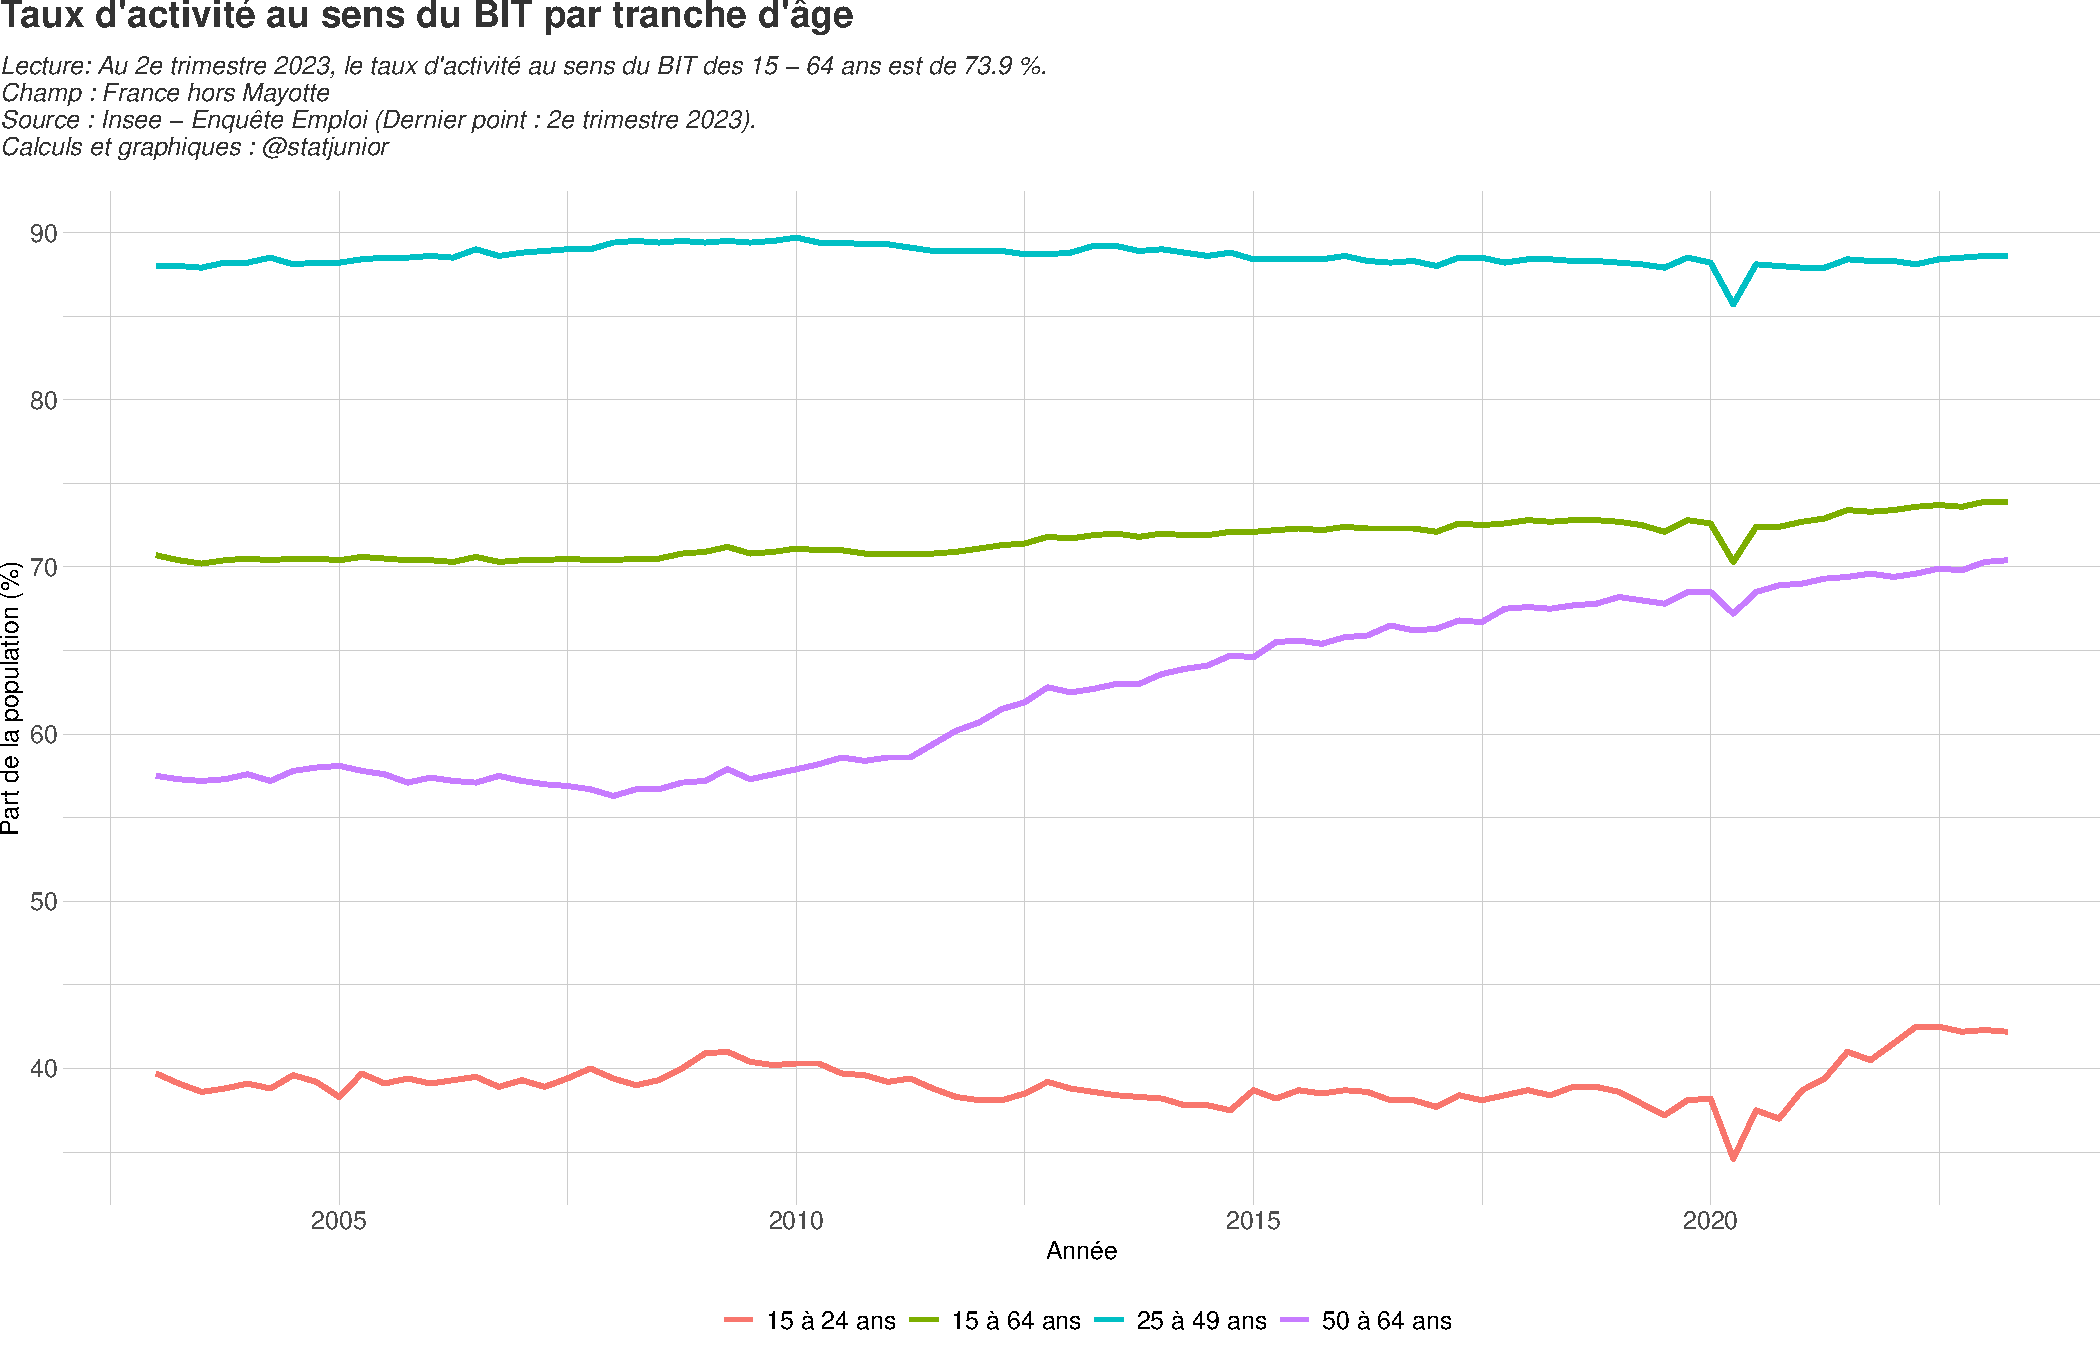
\includegraphics{rapport_activite_emploi_chomage_insee_files/figure-latex/unnamed-chunk-2-1.pdf}

\hypertarget{taux-dactivituxe9-par-sexe}{%
\subsection{Taux d'activité par sexe}\label{taux-dactivituxe9-par-sexe}}

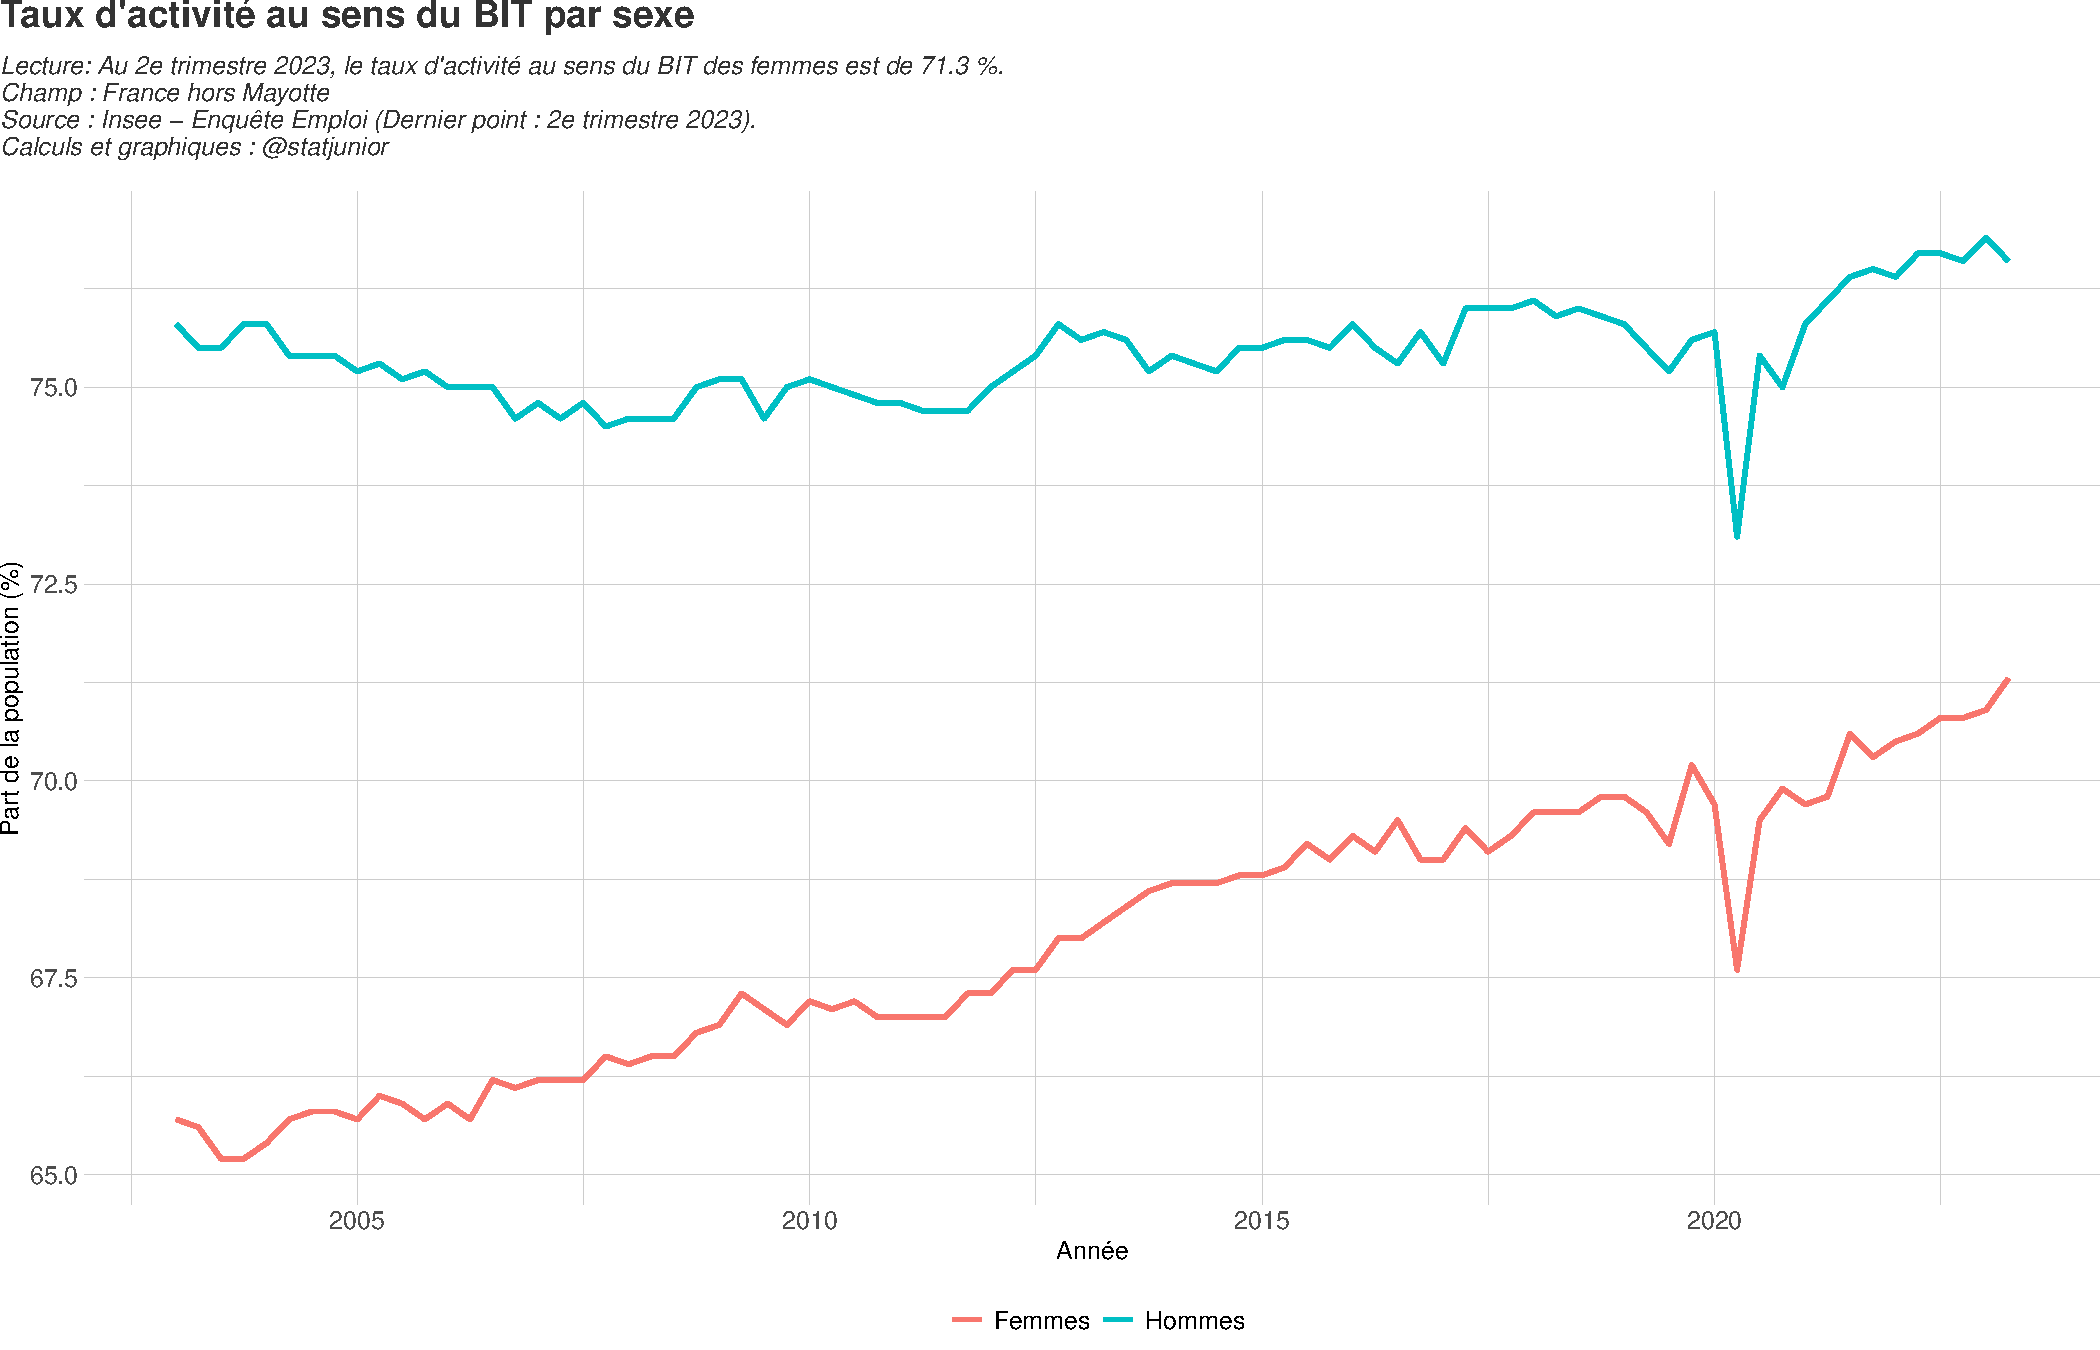
\includegraphics{rapport_activite_emploi_chomage_insee_files/figure-latex/unnamed-chunk-3-1.pdf}

\newpage

\hypertarget{taux-demploi-au-sens-du-bit}{%
\section{Taux d'emploi au sens du
BIT}\label{taux-demploi-au-sens-du-bit}}

Le taux d'emploi au sens du BIT rapporte les personnes en emploi à la
population totale.

\hypertarget{taux-demploi-par-uxe2ge}{%
\subsection{Taux d'emploi par âge}\label{taux-demploi-par-uxe2ge}}

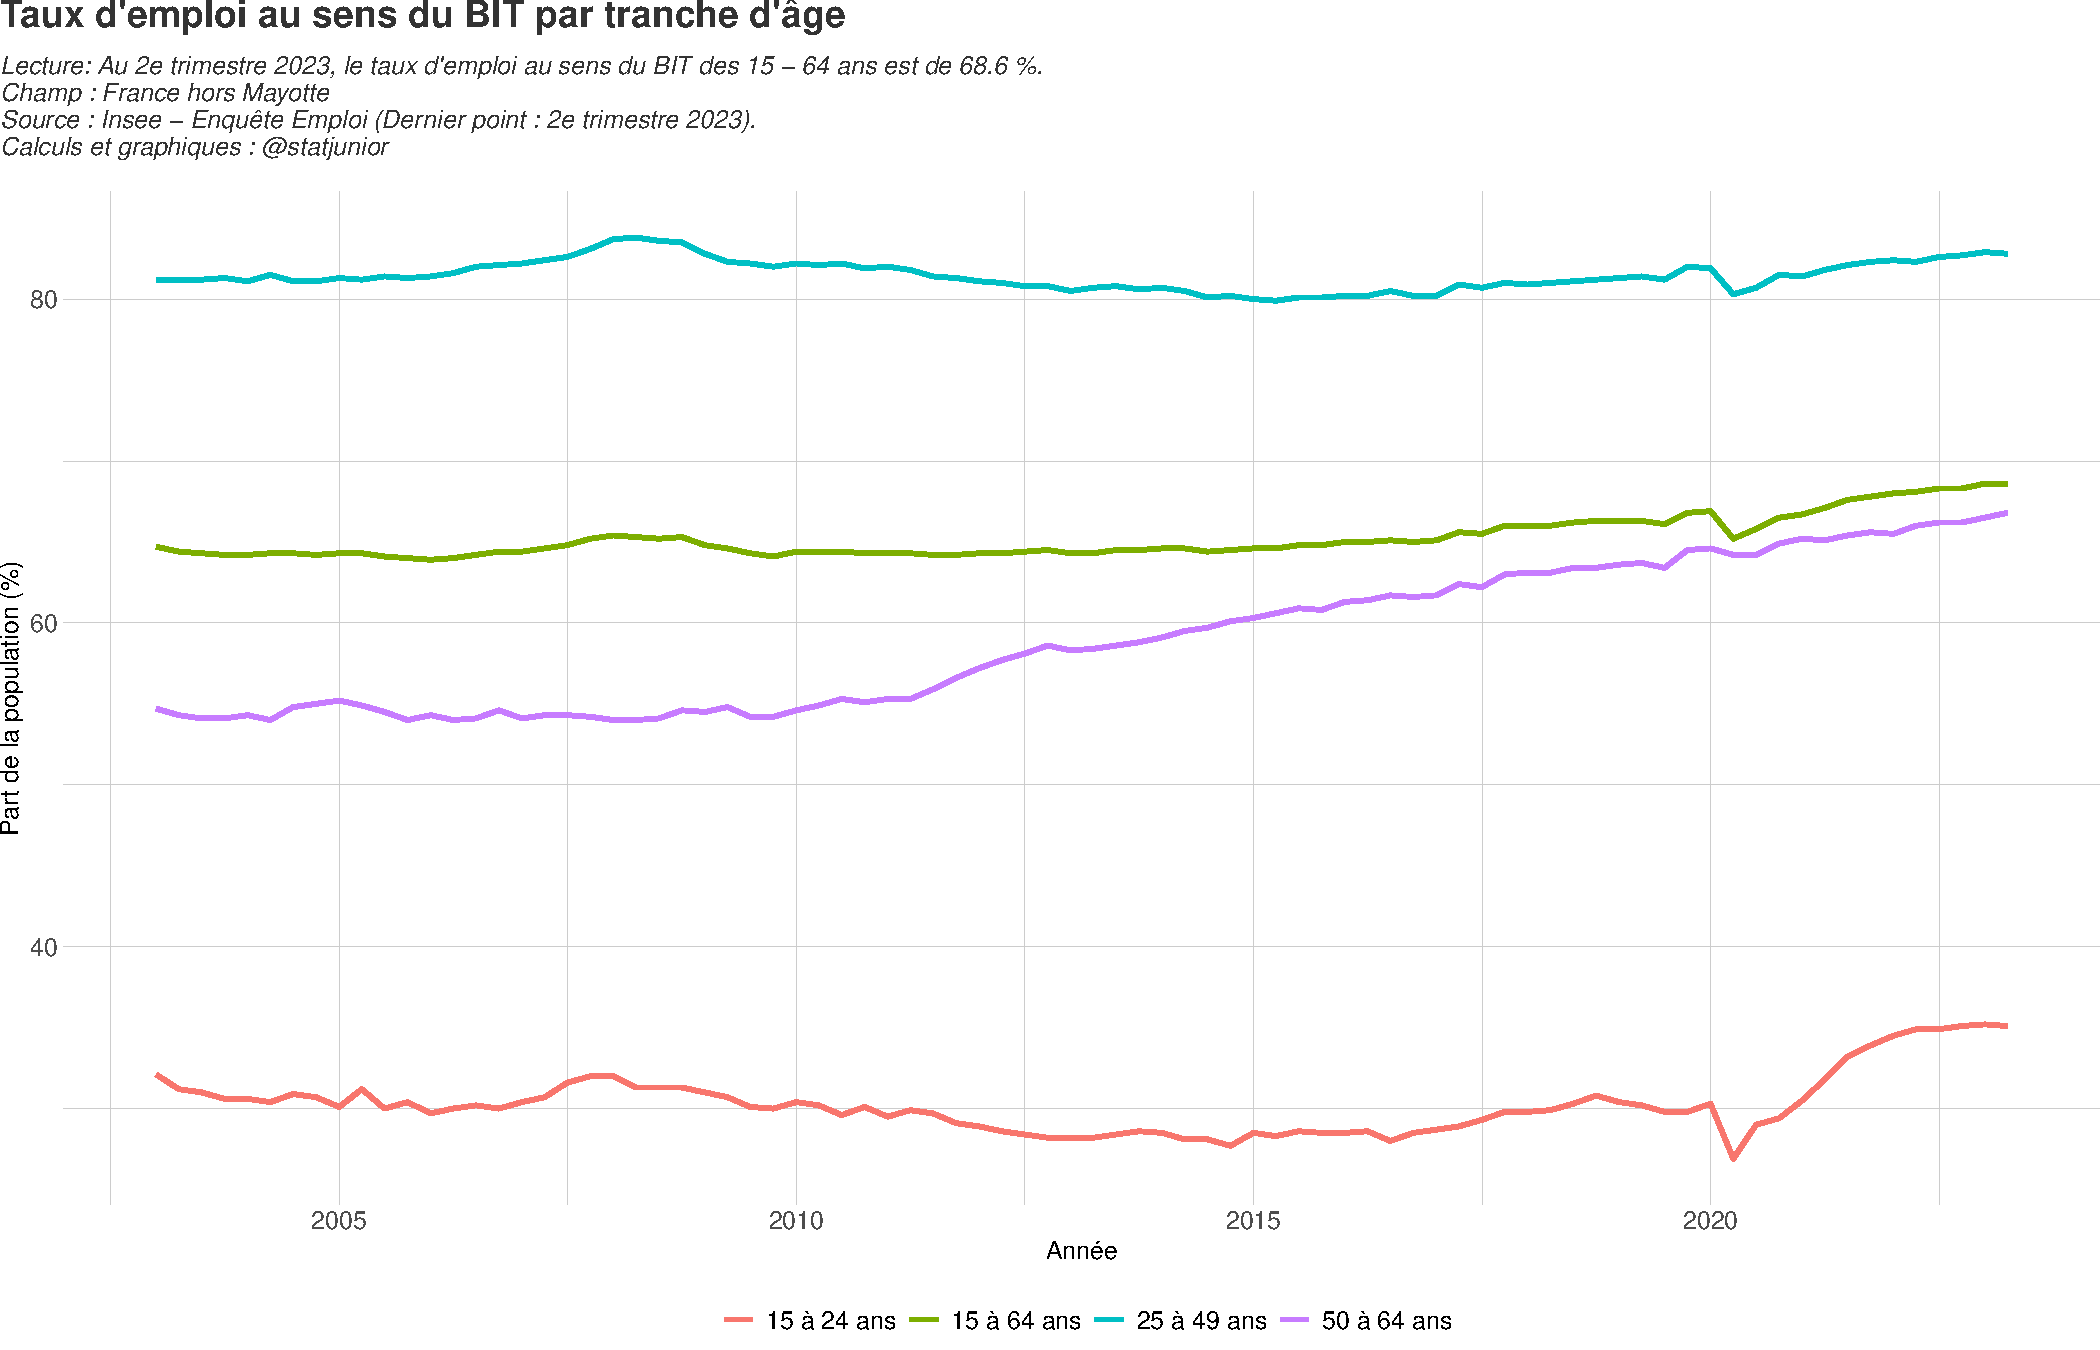
\includegraphics{rapport_activite_emploi_chomage_insee_files/figure-latex/unnamed-chunk-4-1.pdf}

\hypertarget{taux-demploi-par-sexe}{%
\subsection{Taux d'emploi par sexe}\label{taux-demploi-par-sexe}}

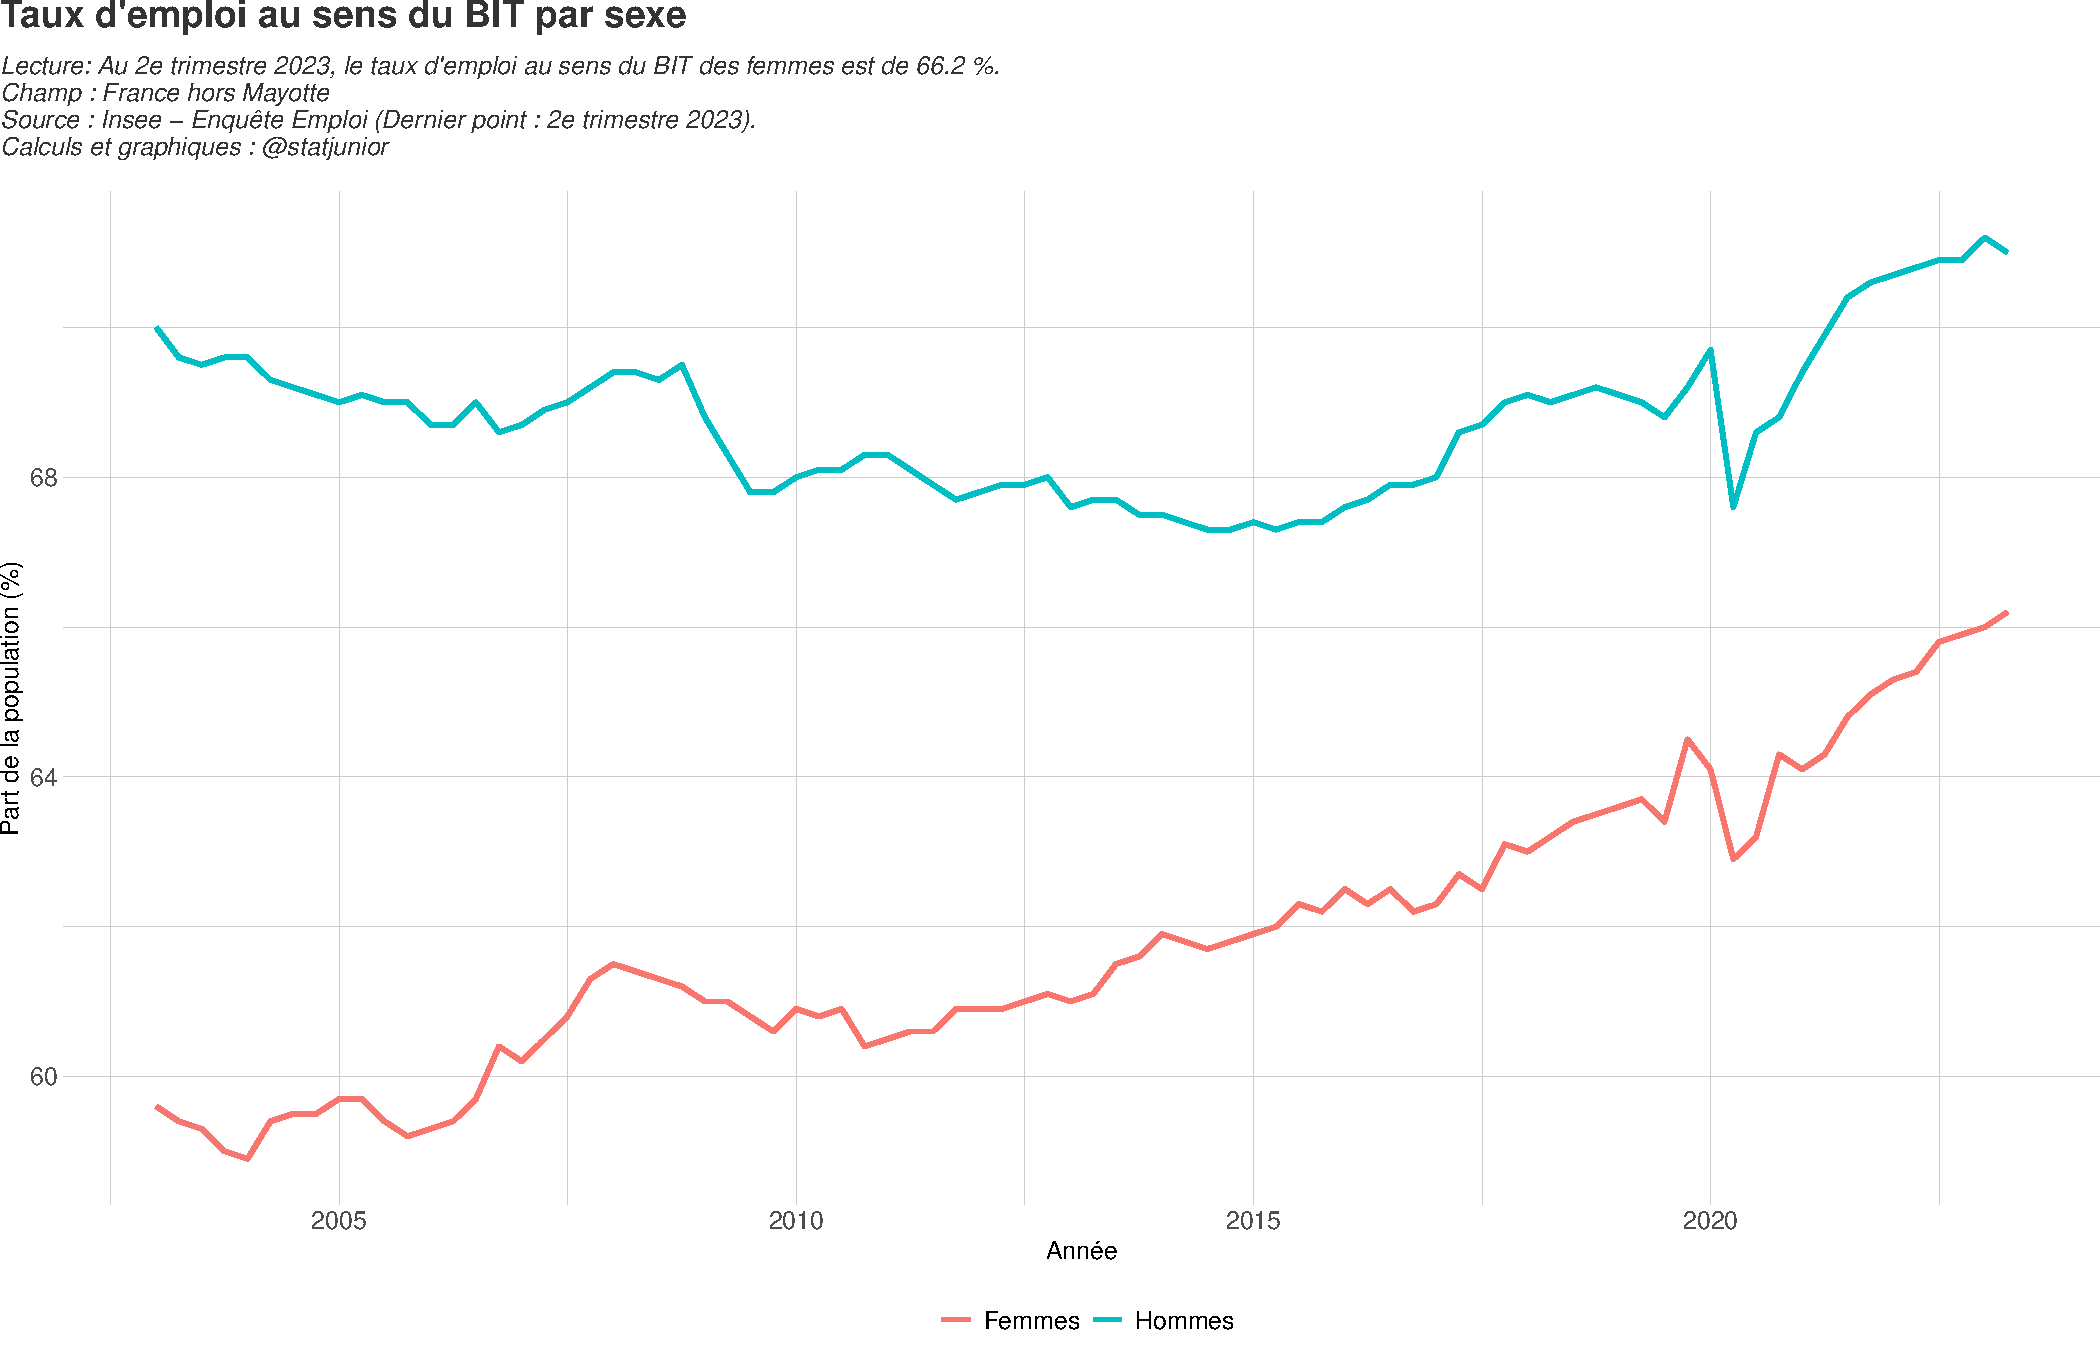
\includegraphics{rapport_activite_emploi_chomage_insee_files/figure-latex/unnamed-chunk-5-1.pdf}

\newpage

\hypertarget{taux-demploi-par-catuxe9gorie}{%
\section{Taux d'emploi par
catégorie}\label{taux-demploi-par-catuxe9gorie}}

\hypertarget{temps-de-travail}{%
\subsection{Temps de travail}\label{temps-de-travail}}

\hypertarget{taux-demploi-uxe0-temps-complet-par-uxe2ge}{%
\subsubsection{Taux d'emploi à temps complet par
âge}\label{taux-demploi-uxe0-temps-complet-par-uxe2ge}}

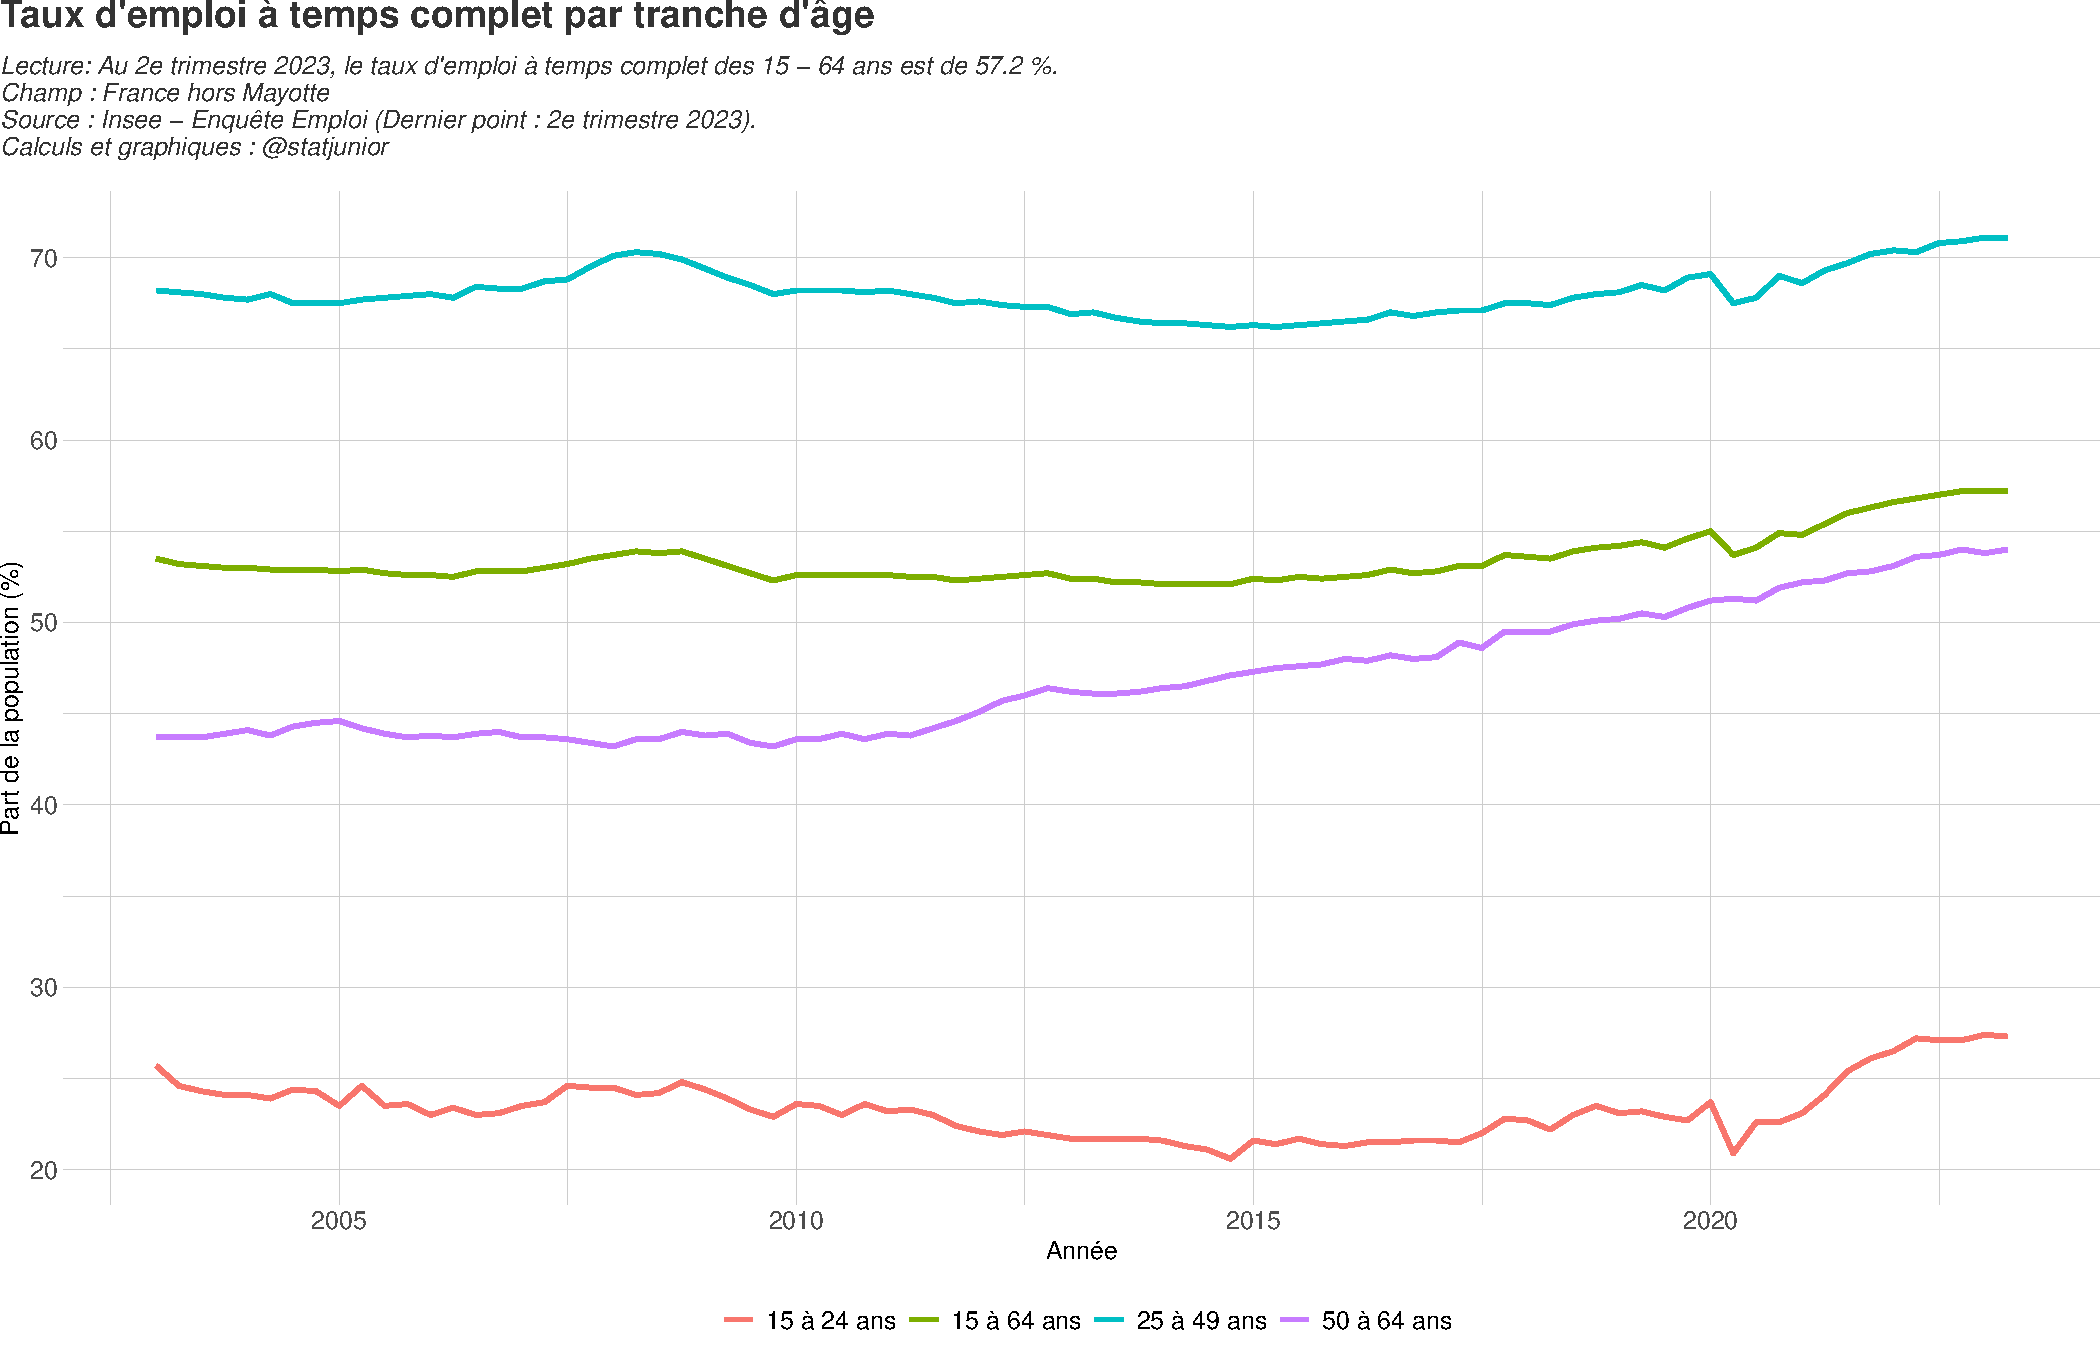
\includegraphics{rapport_activite_emploi_chomage_insee_files/figure-latex/unnamed-chunk-6-1.pdf}

\hypertarget{taux-demploi-uxe0-temps-complet-par-sexe}{%
\subsubsection{Taux d'emploi à temps complet par
sexe}\label{taux-demploi-uxe0-temps-complet-par-sexe}}

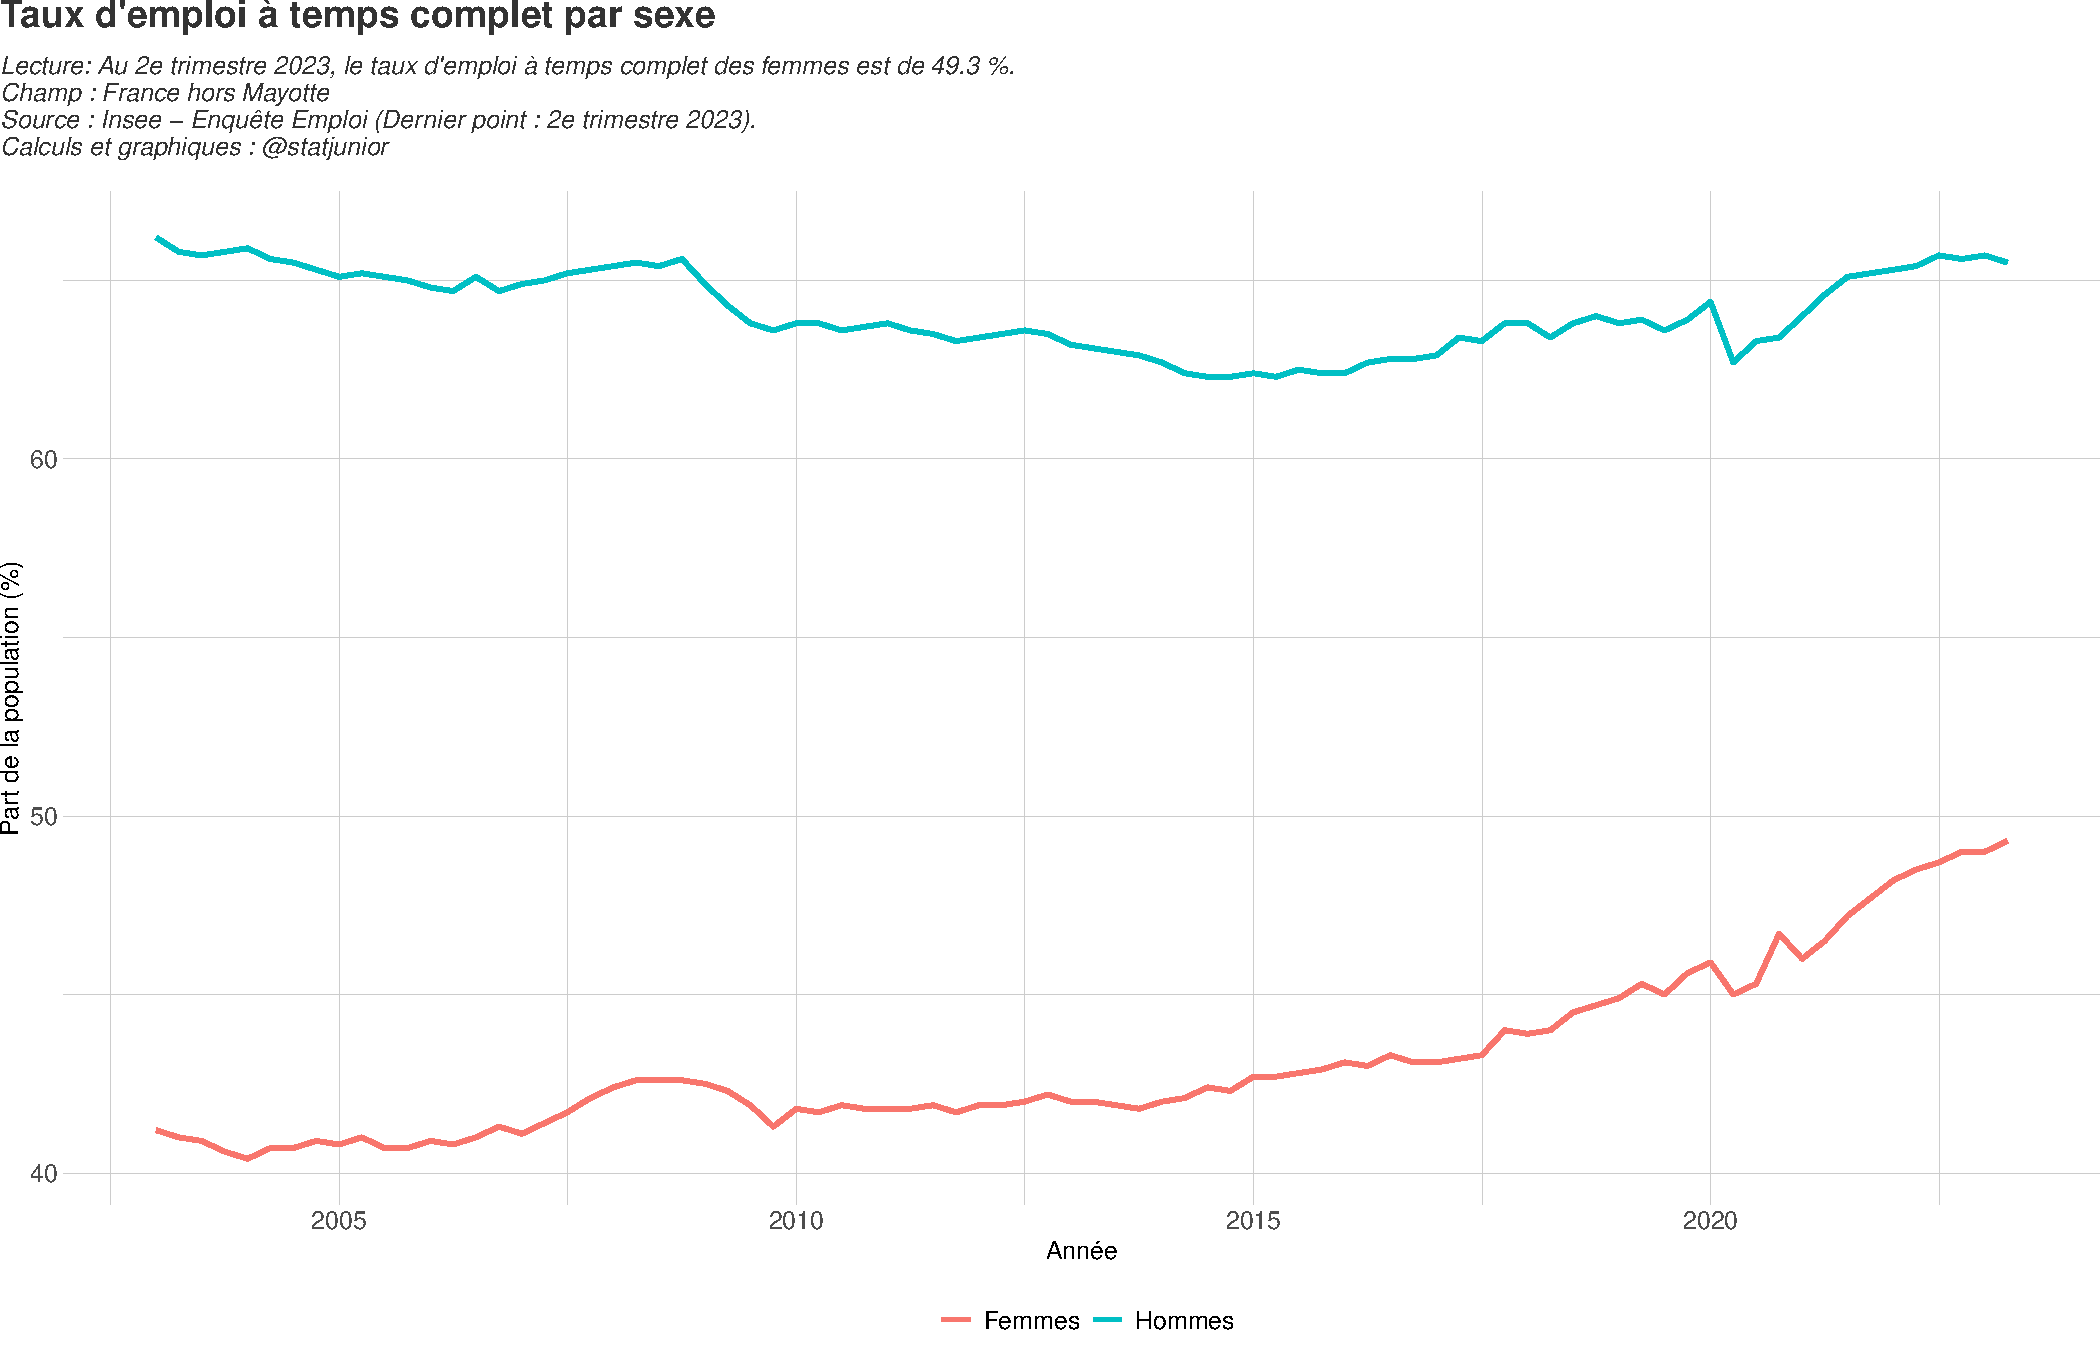
\includegraphics{rapport_activite_emploi_chomage_insee_files/figure-latex/unnamed-chunk-7-1.pdf}

\hypertarget{taux-demploi-uxe0-temps-partiel}{%
\subsection{Taux d'emploi à temps
partiel}\label{taux-demploi-uxe0-temps-partiel}}

\hypertarget{taux-demploi-uxe0-temps-partiel-par-uxe2ge}{%
\subsubsection{Taux d'emploi à temps partiel par
âge}\label{taux-demploi-uxe0-temps-partiel-par-uxe2ge}}

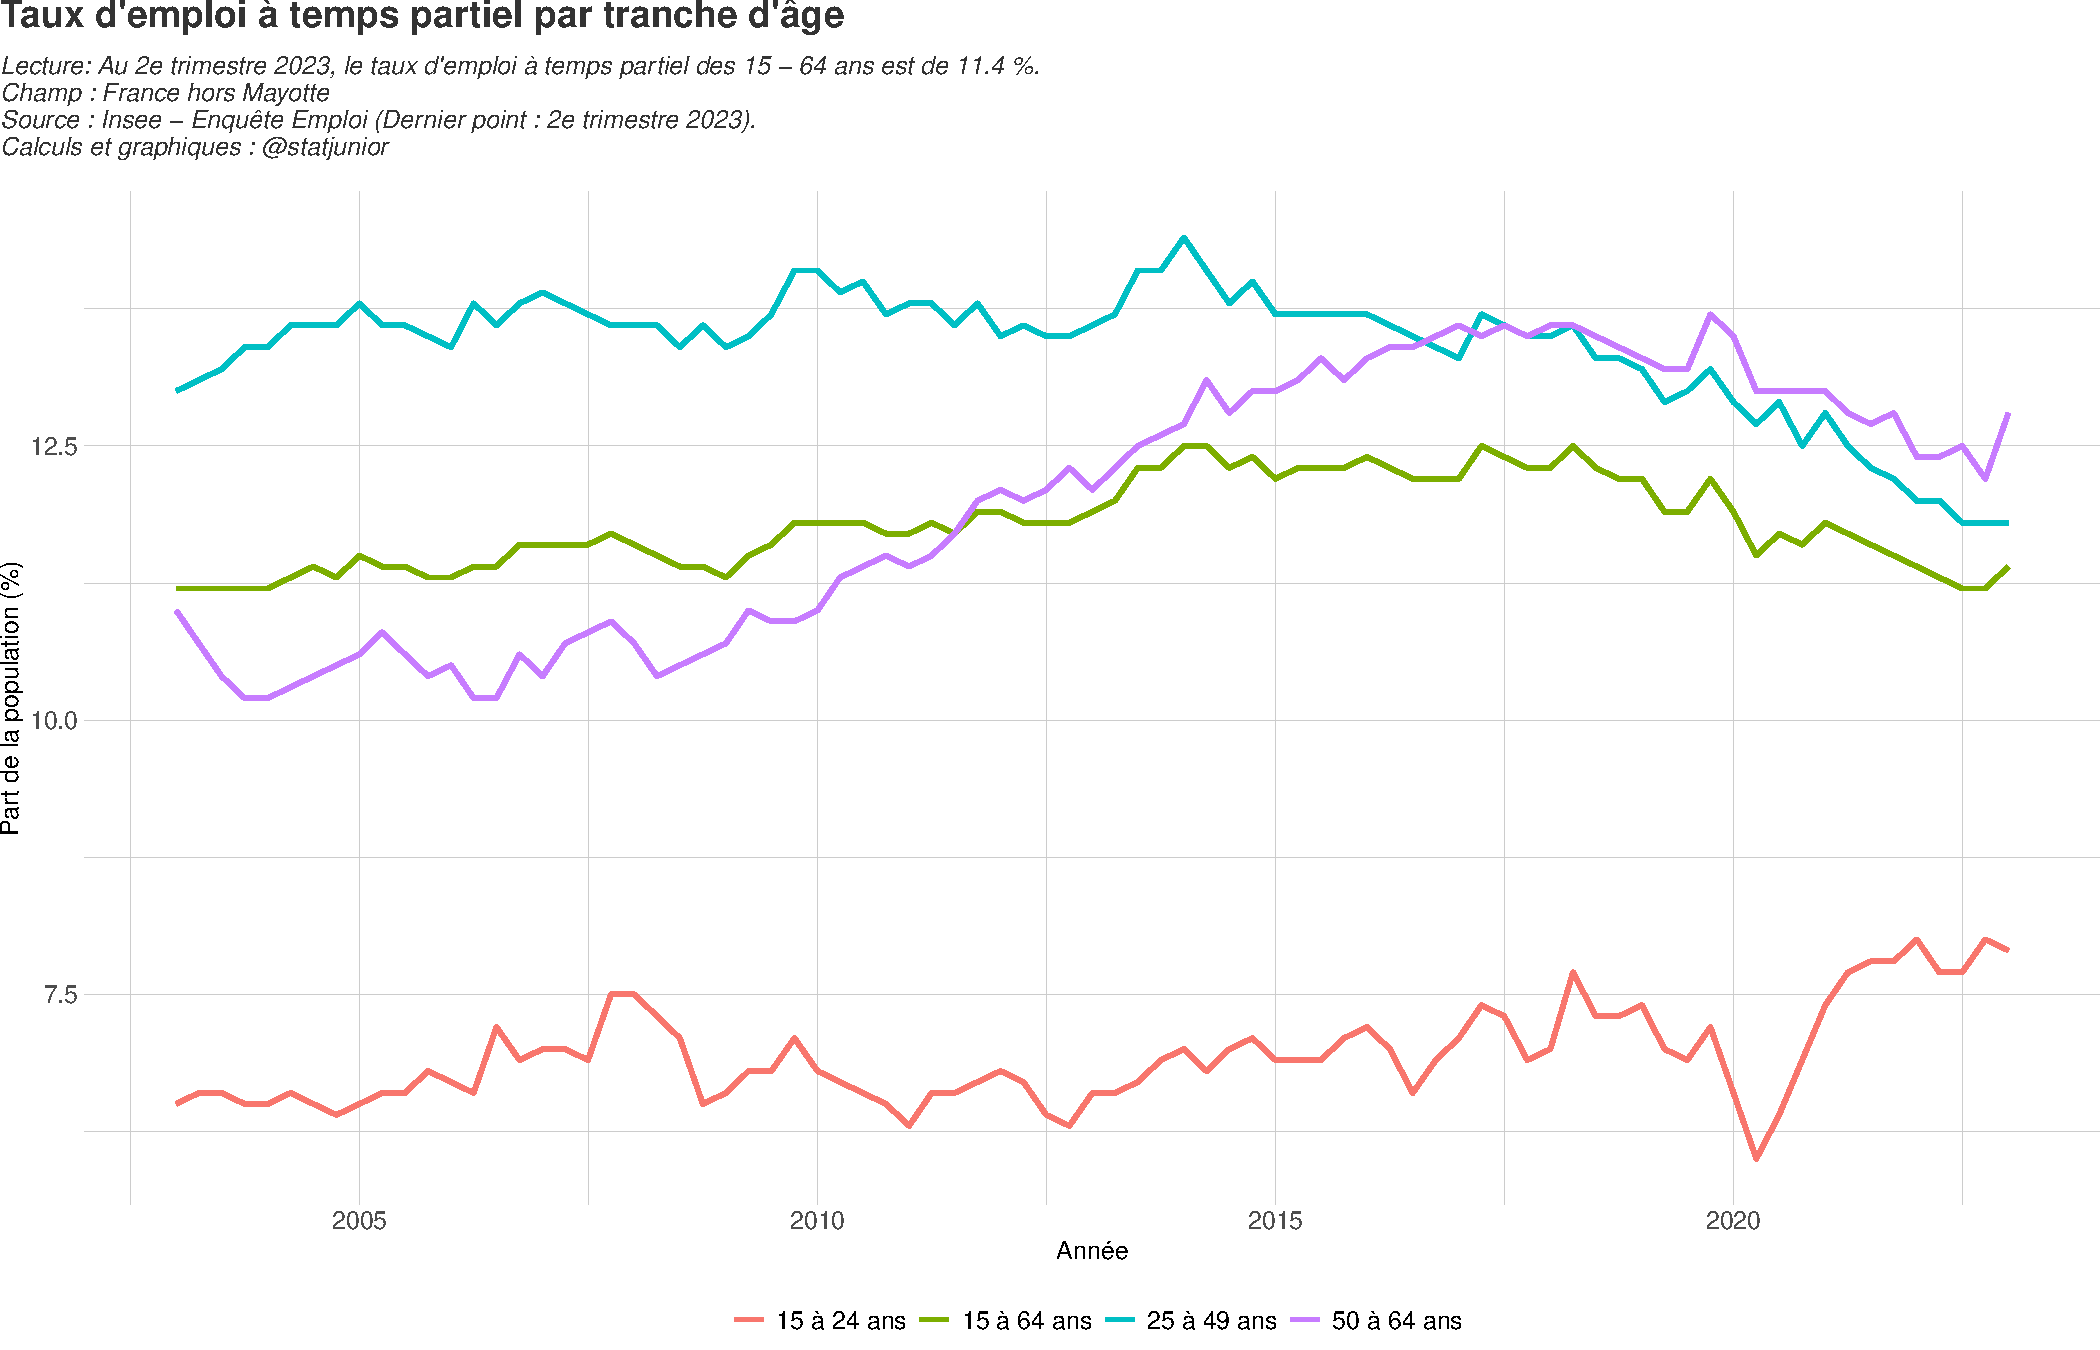
\includegraphics{rapport_activite_emploi_chomage_insee_files/figure-latex/unnamed-chunk-8-1.pdf}

\hypertarget{taux-demploi-uxe0-temps-partiel-par-sexe}{%
\subsubsection{Taux d'emploi à temps partiel par
sexe}\label{taux-demploi-uxe0-temps-partiel-par-sexe}}

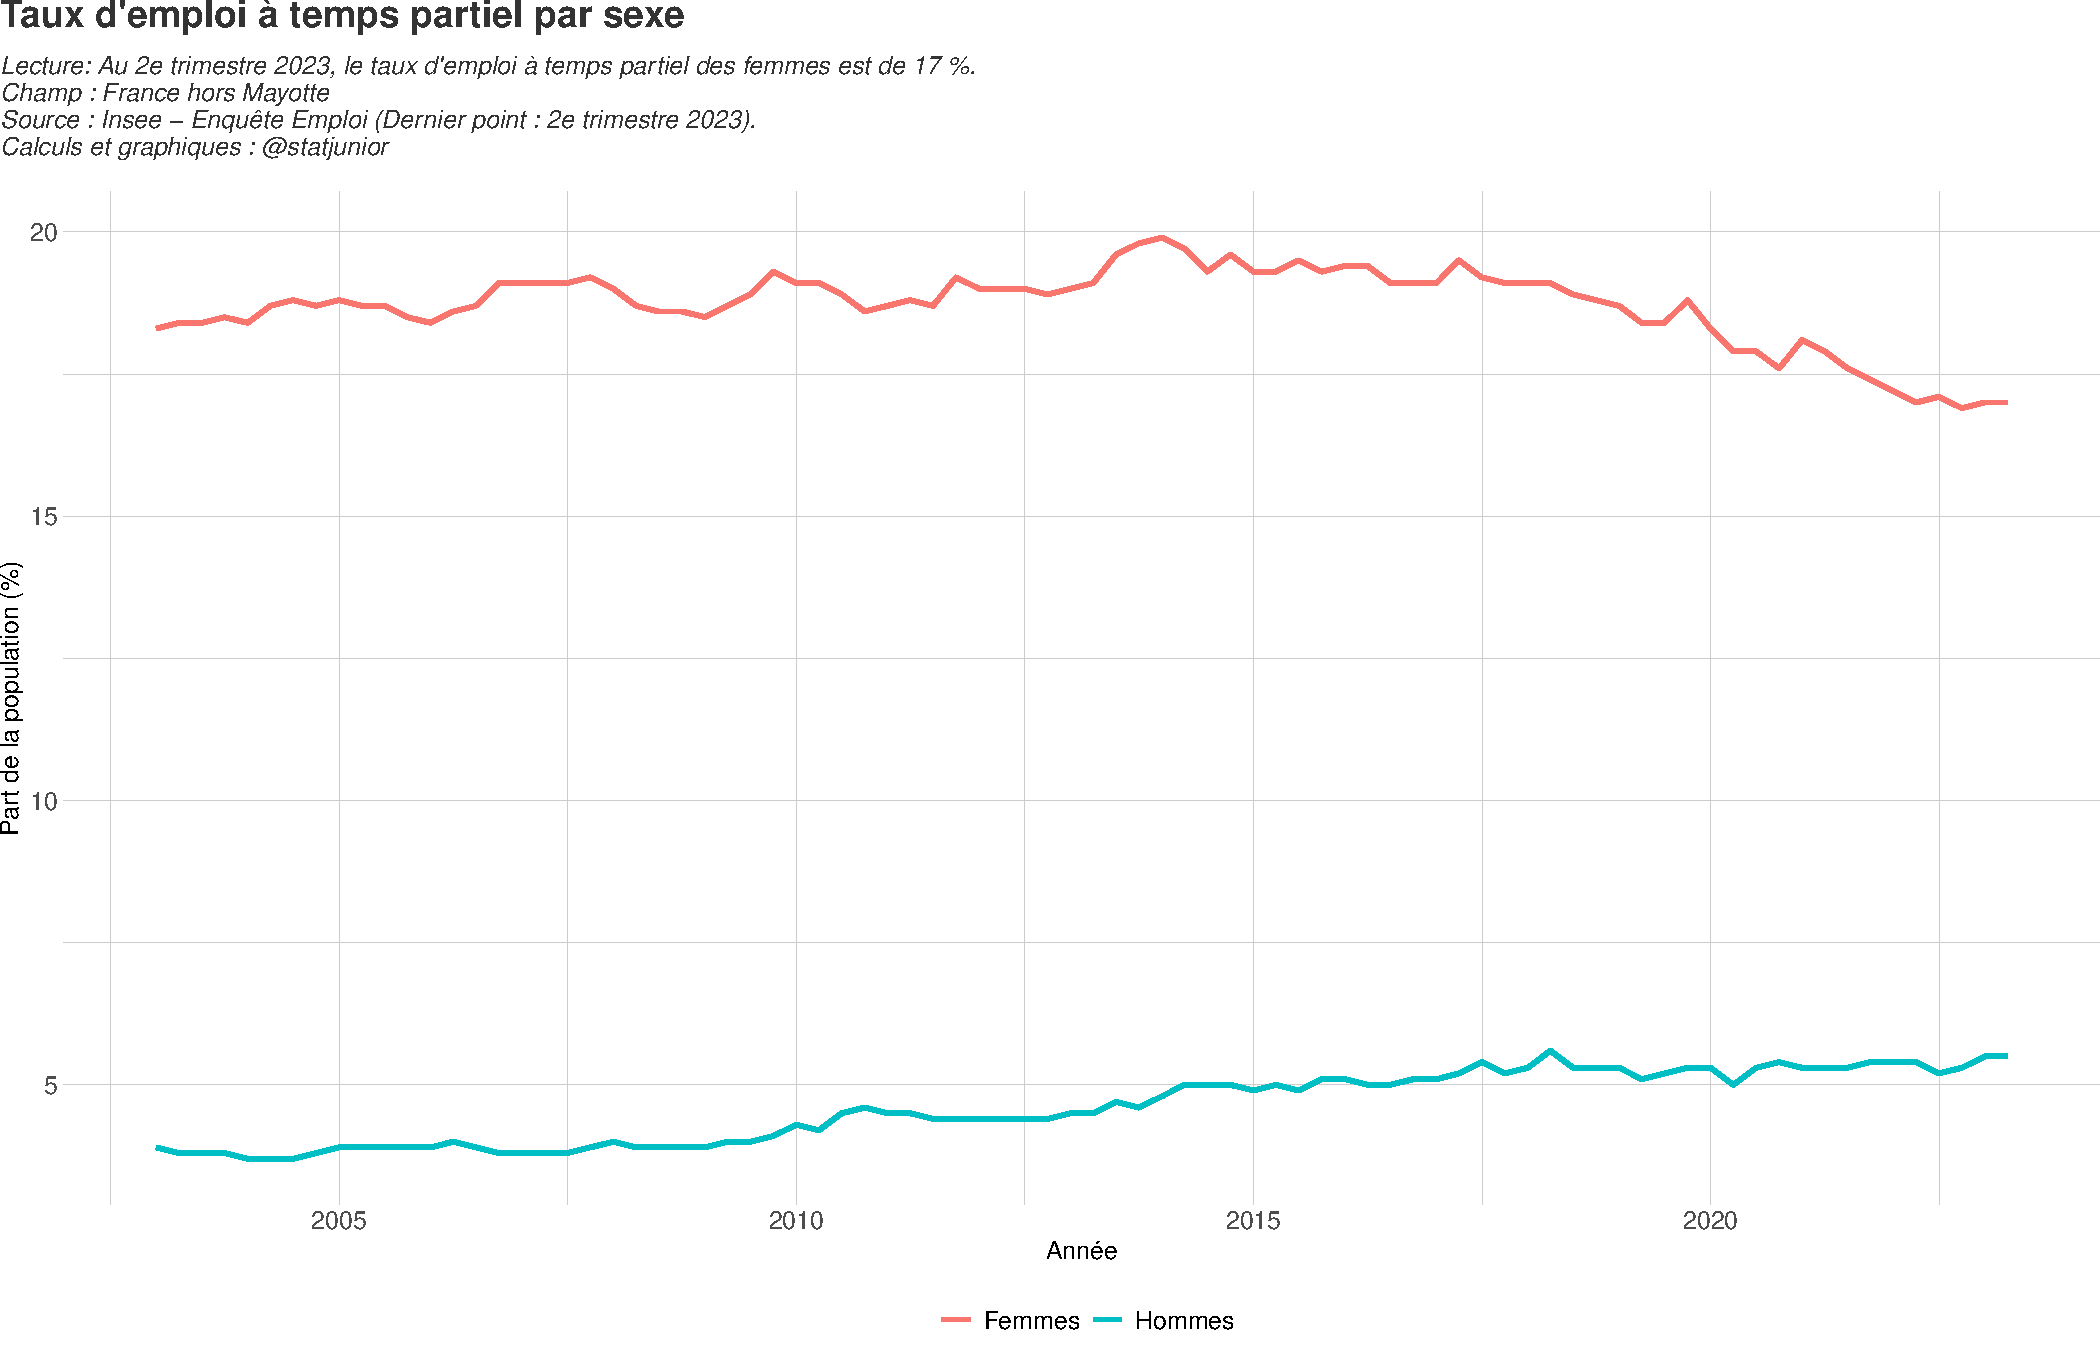
\includegraphics{rapport_activite_emploi_chomage_insee_files/figure-latex/unnamed-chunk-9-1.pdf}

\hypertarget{taux-demploi-en-equivalent-temps-plein-eqtp}{%
\subsection{Taux d'emploi en Equivalent Temps Plein
(EQTP)}\label{taux-demploi-en-equivalent-temps-plein-eqtp}}

\hypertarget{taux-demploi-en-eqtp-par-uxe2ge}{%
\subsubsection{Taux d'emploi en EQTP par
âge}\label{taux-demploi-en-eqtp-par-uxe2ge}}

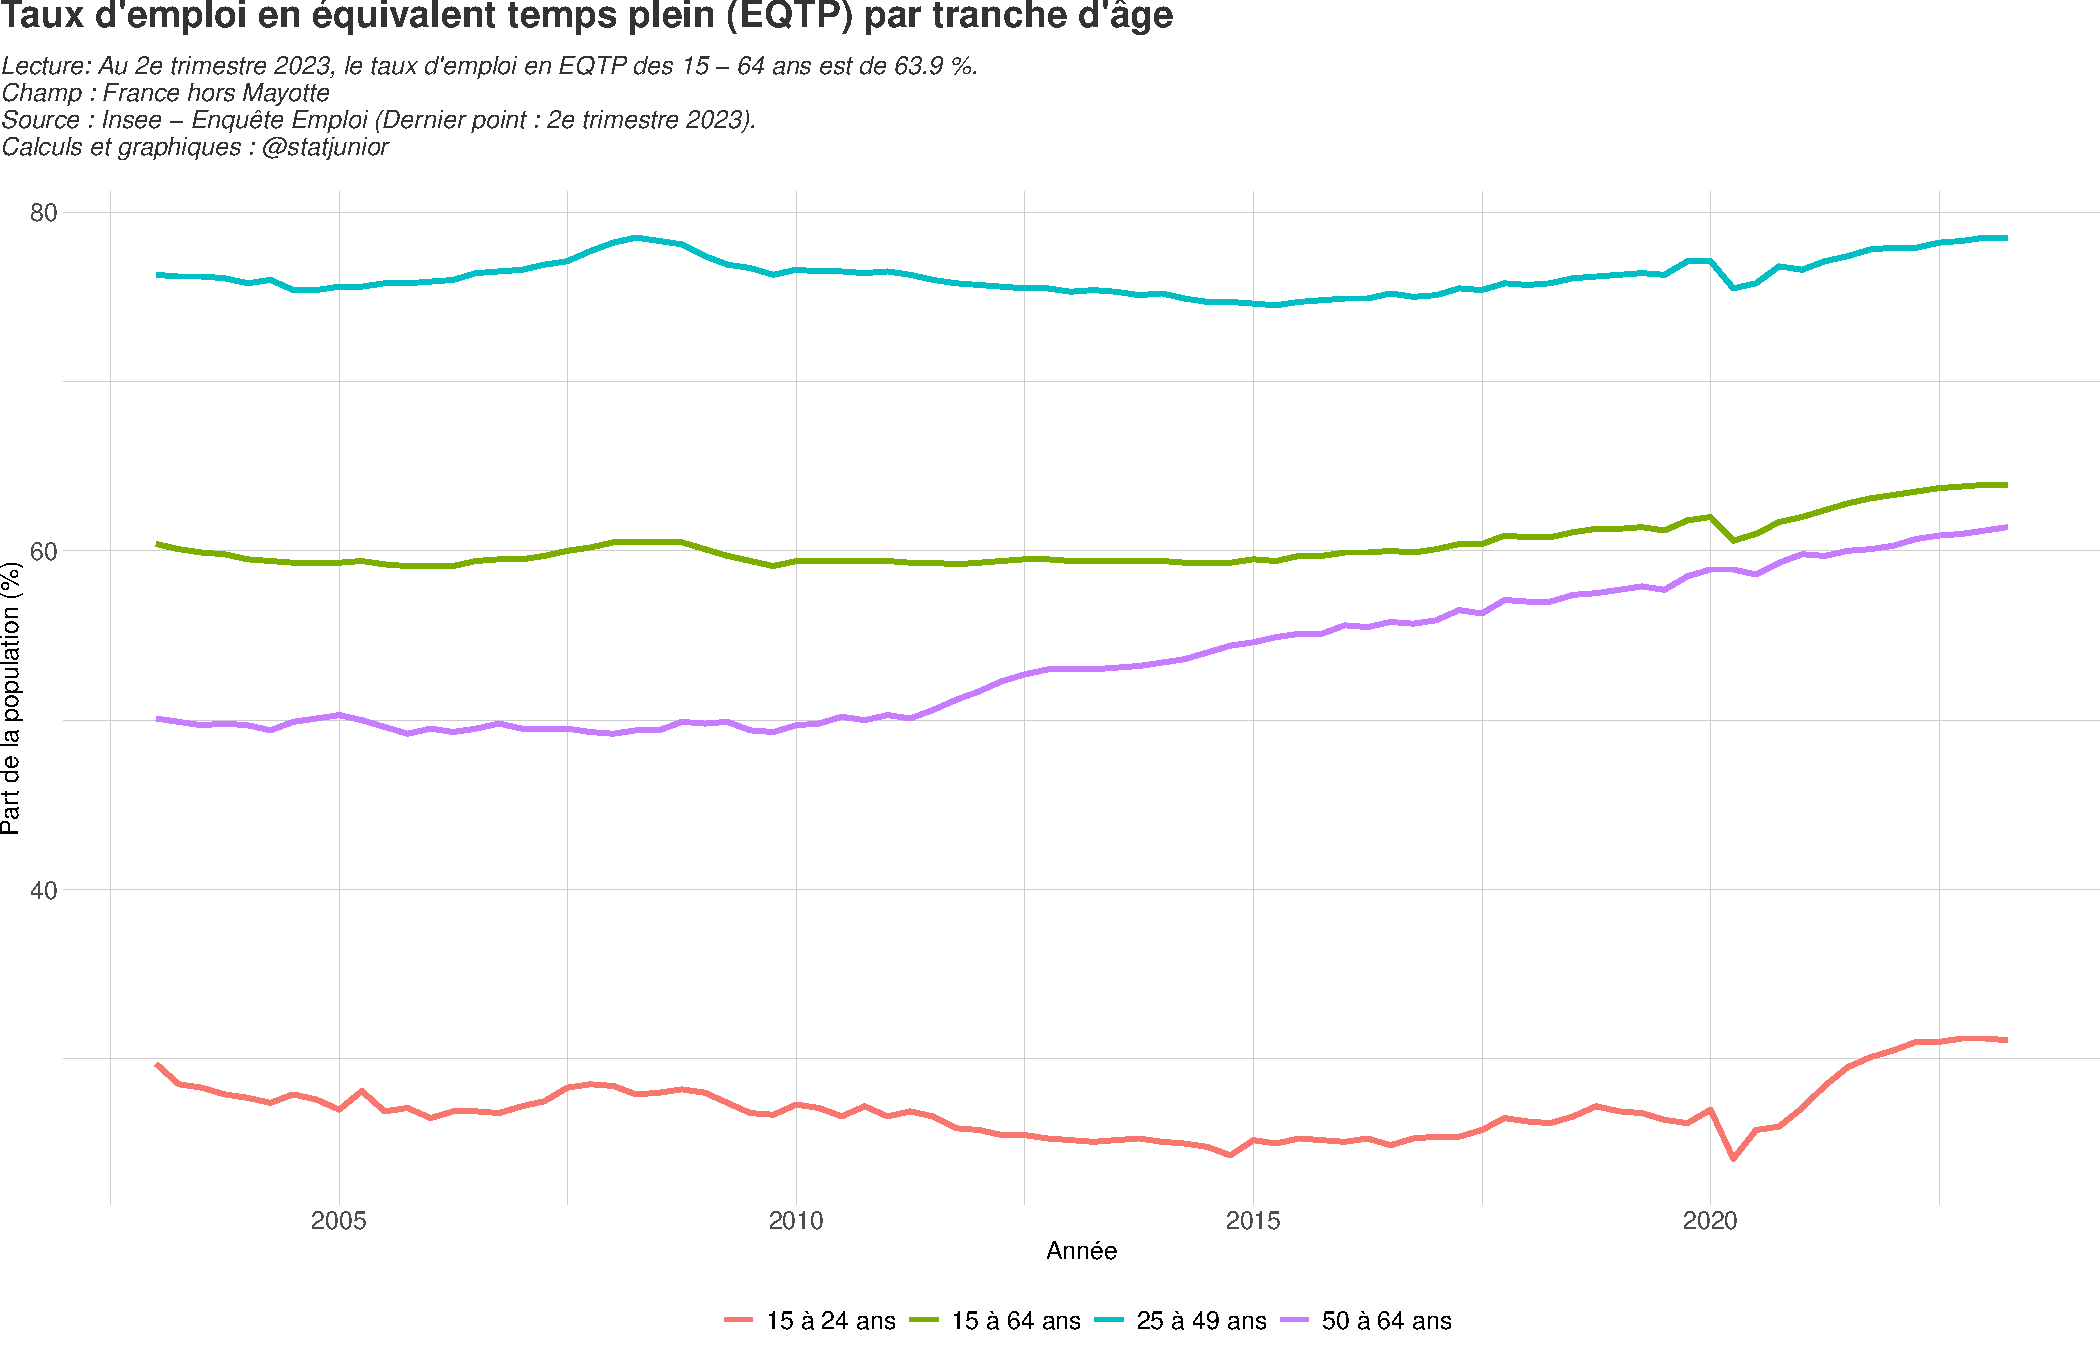
\includegraphics{rapport_activite_emploi_chomage_insee_files/figure-latex/unnamed-chunk-10-1.pdf}

\hypertarget{taux-demploi-en-eqtp-par-sexe}{%
\subsubsection{Taux d'emploi en EQTP par
sexe}\label{taux-demploi-en-eqtp-par-sexe}}

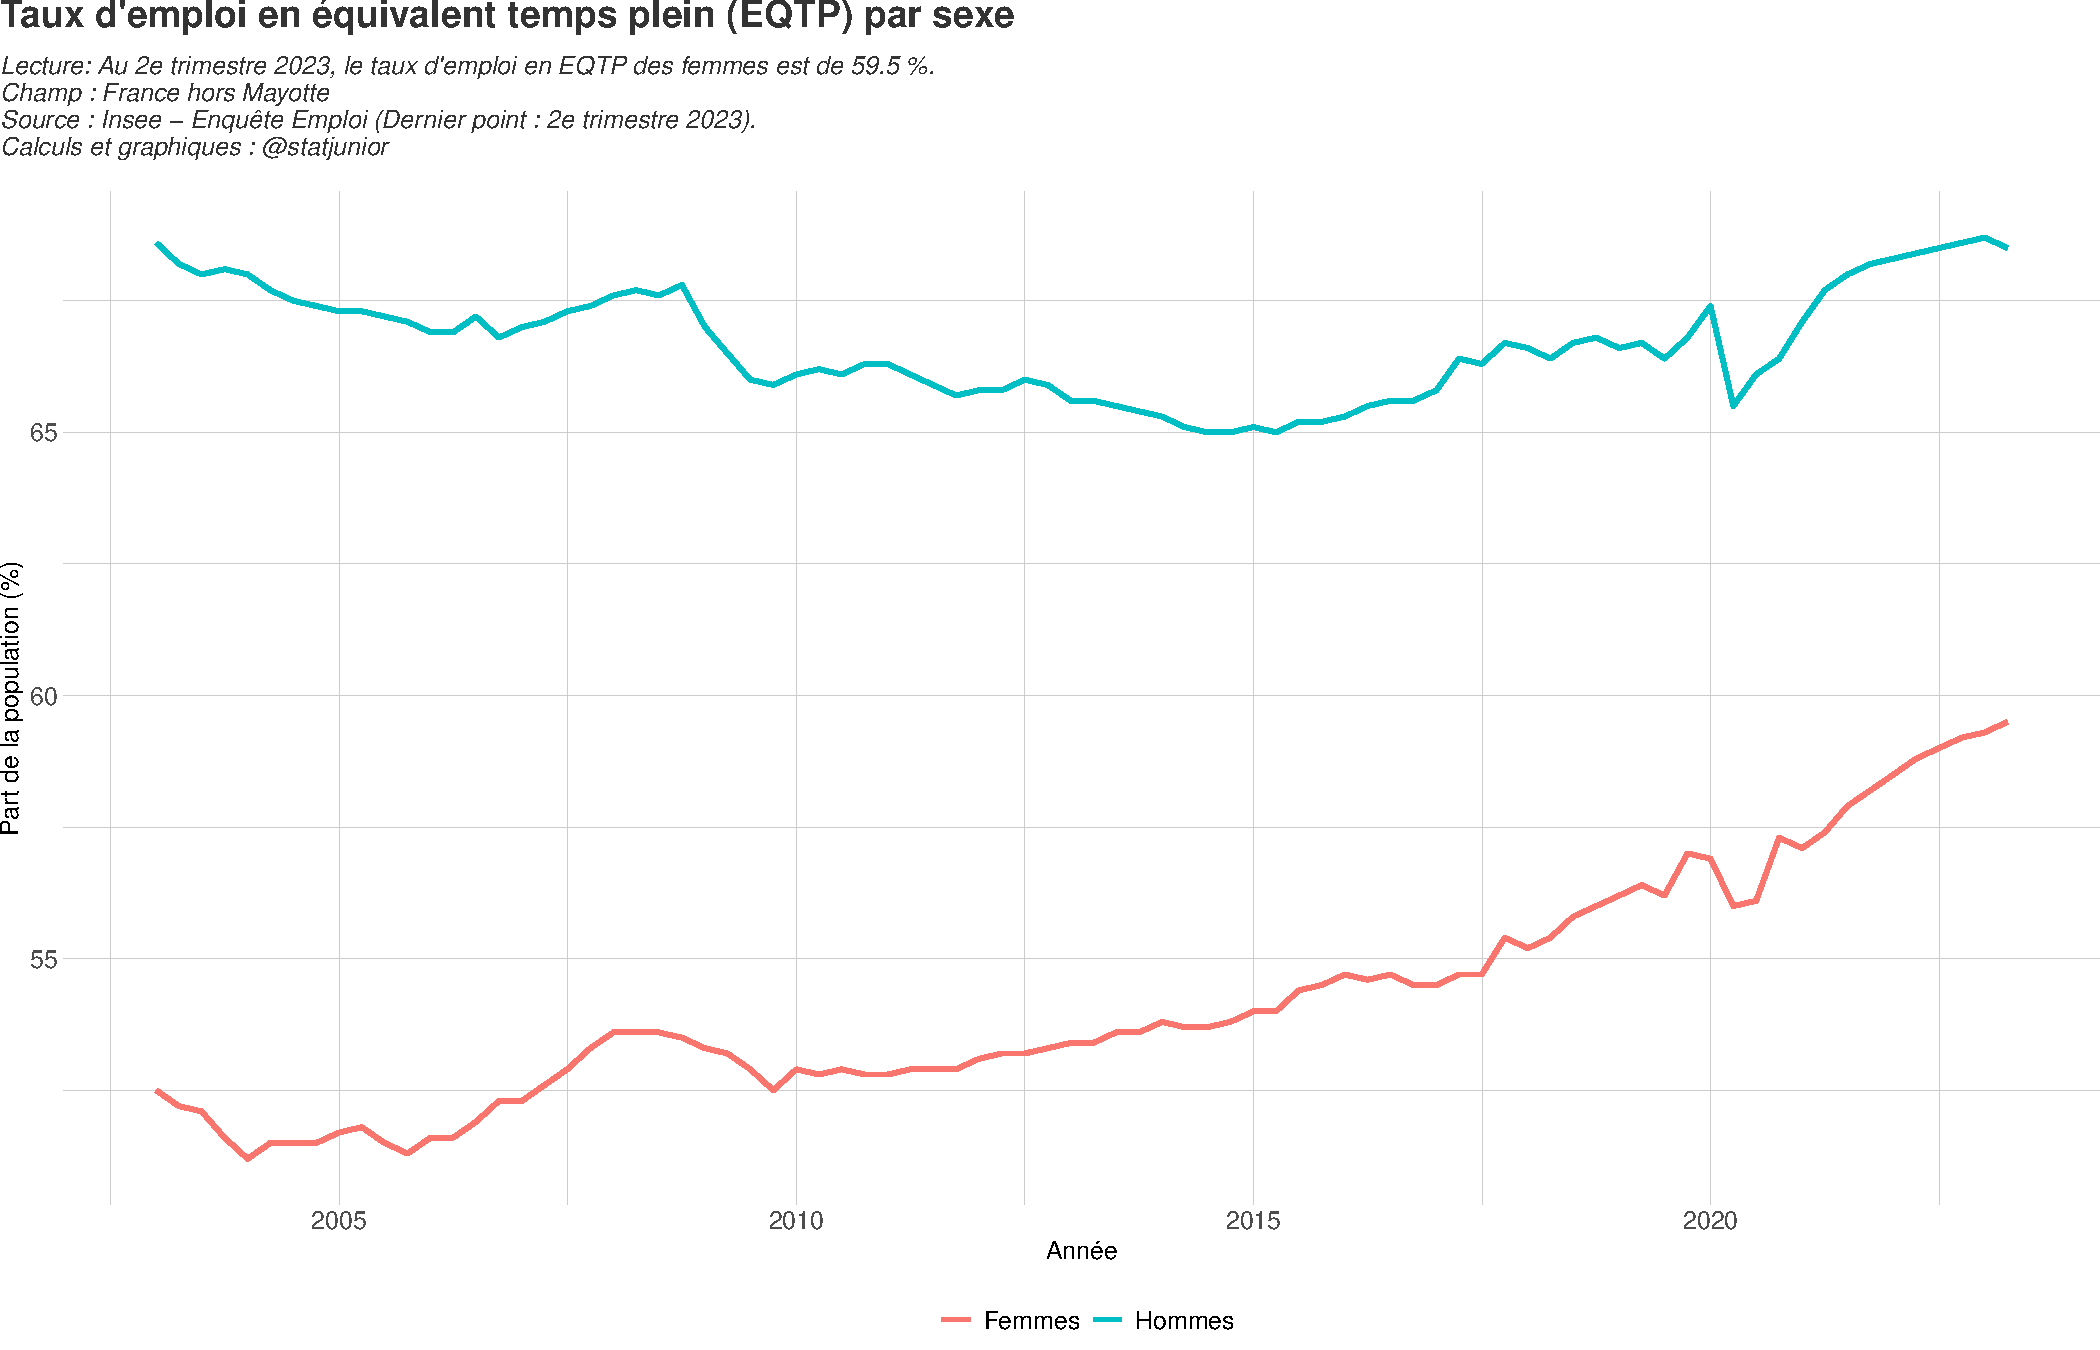
\includegraphics{rapport_activite_emploi_chomage_insee_files/figure-latex/unnamed-chunk-11-1.pdf}

\hypertarget{contribution-du-sous-emploi-au-taux-demploi-total}{%
\subsection{Contribution du Sous-emploi au taux d'emploi
total}\label{contribution-du-sous-emploi-au-taux-demploi-total}}

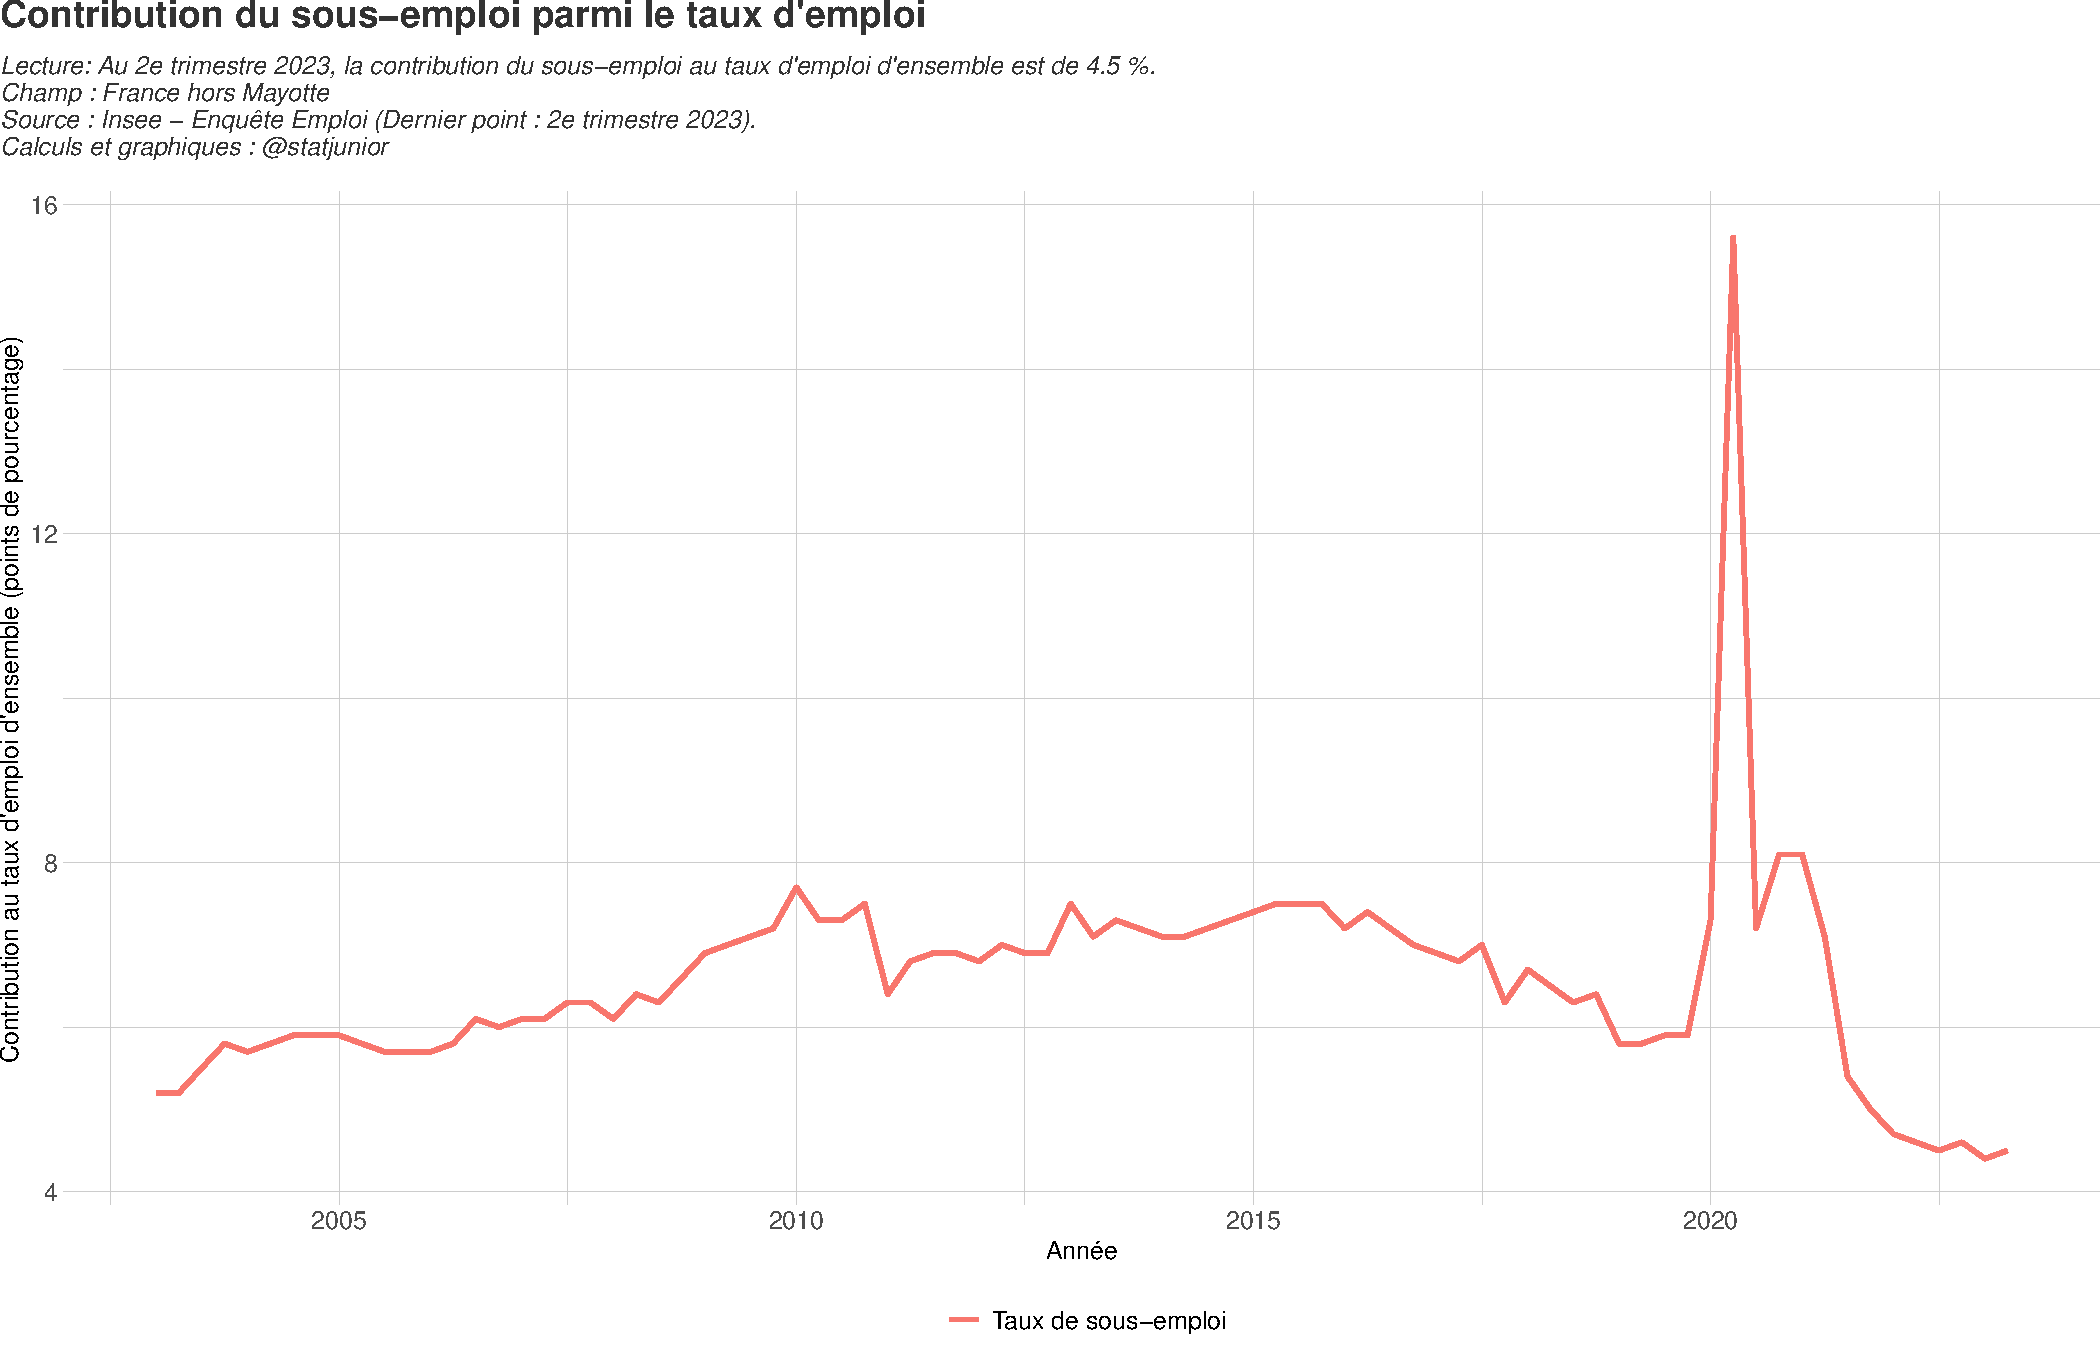
\includegraphics{rapport_activite_emploi_chomage_insee_files/figure-latex/unnamed-chunk-12-1.pdf}

\hypertarget{taux-demploi-en-cdd-ou-en-intuxe9rim}{%
\subsection{Taux d'emploi en CDD ou en
intérim}\label{taux-demploi-en-cdd-ou-en-intuxe9rim}}

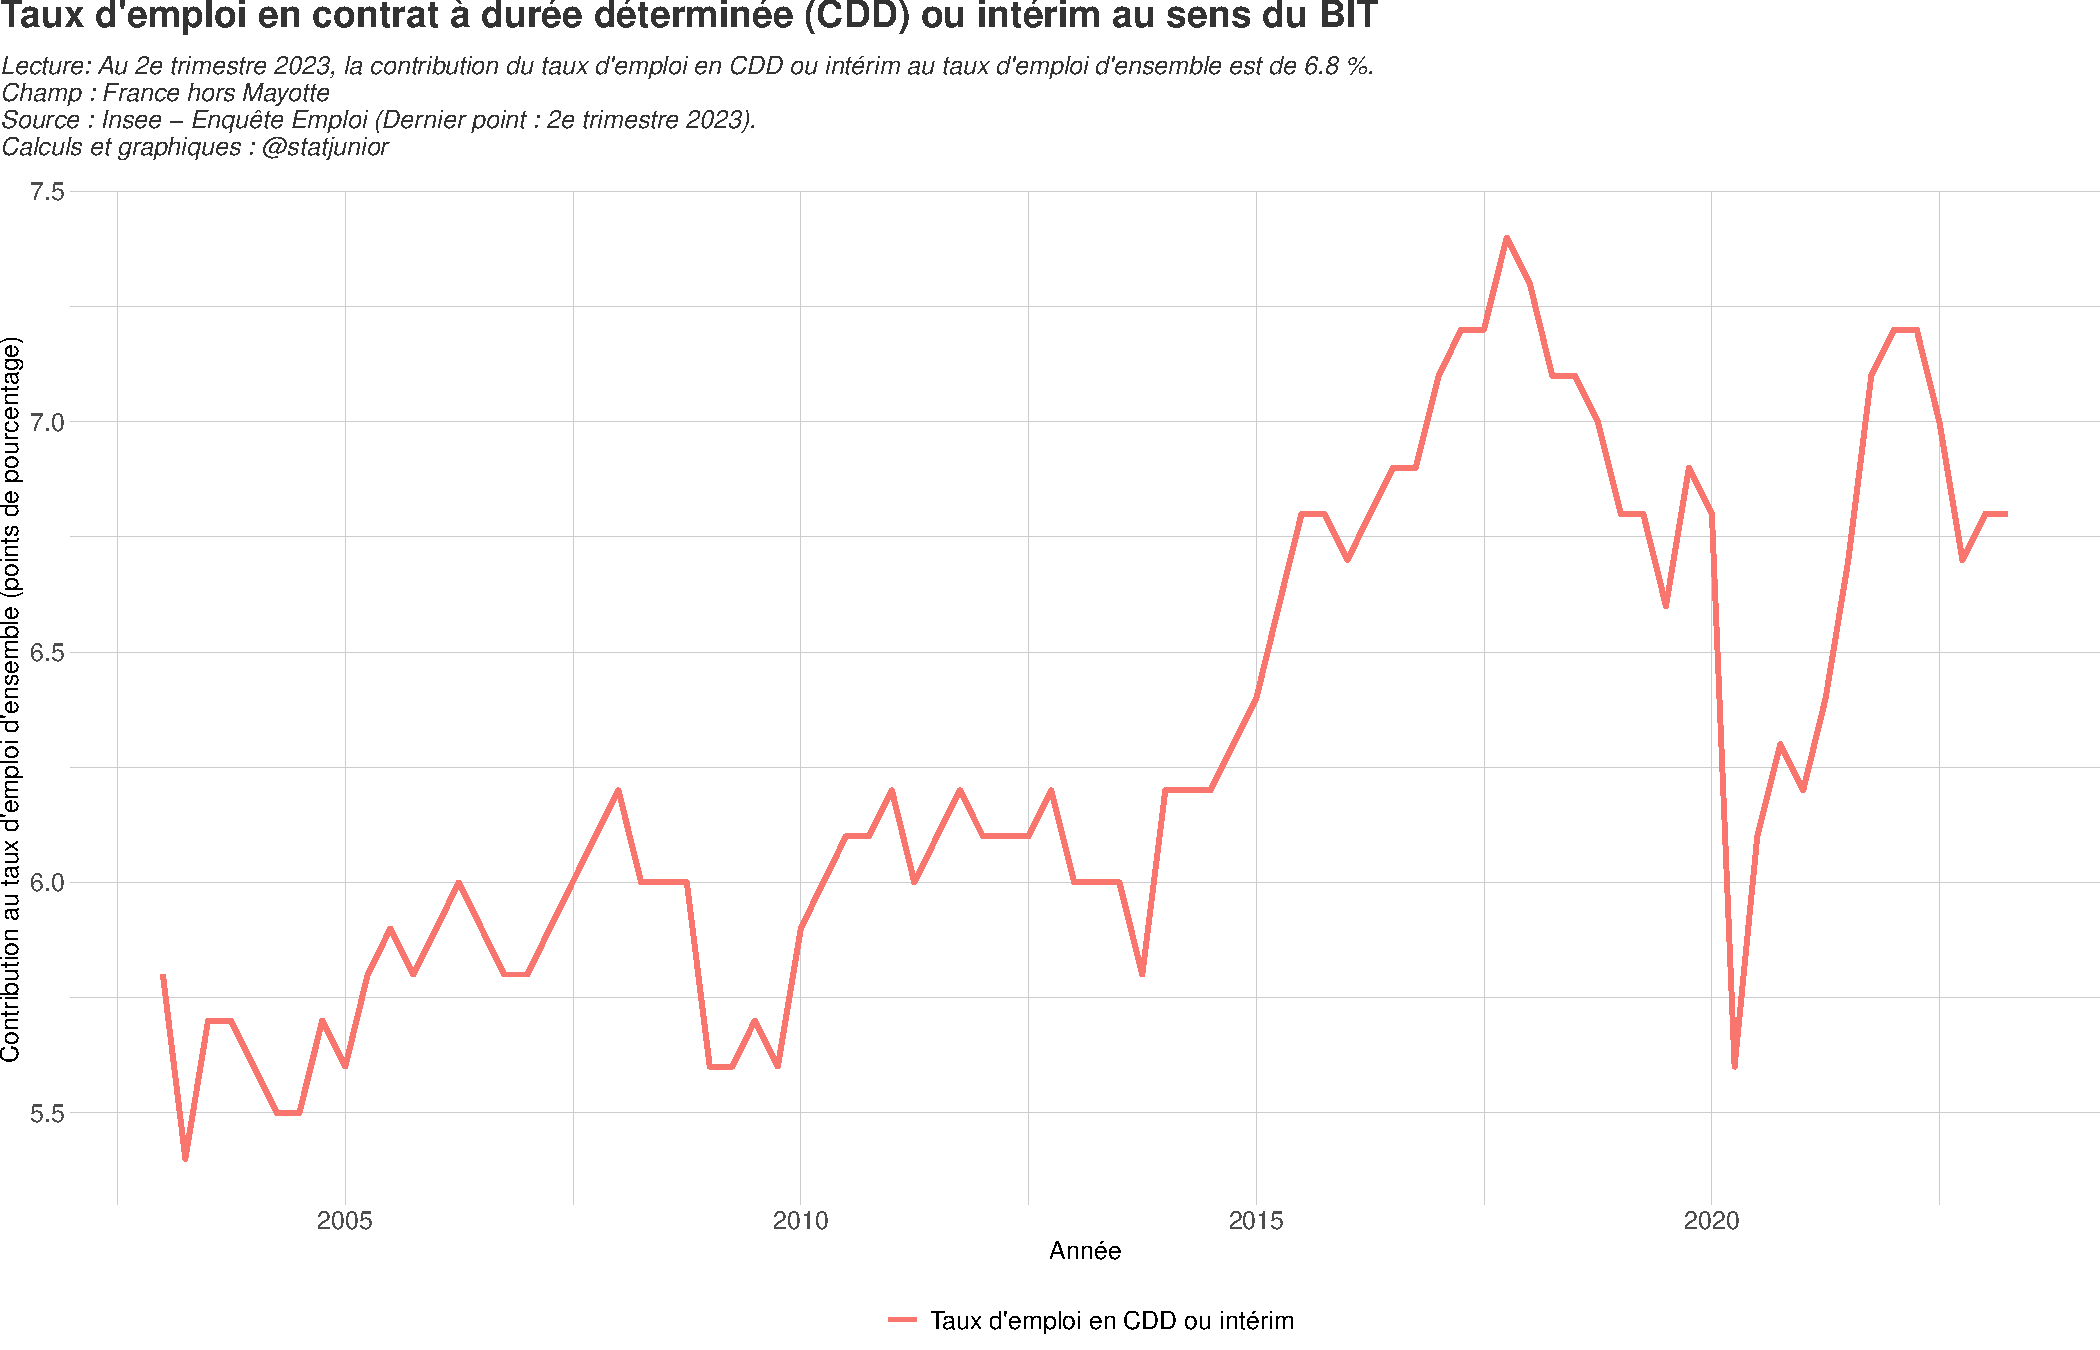
\includegraphics{rapport_activite_emploi_chomage_insee_files/figure-latex/unnamed-chunk-13-1.pdf}

\hypertarget{nombre-moyen-dheures-travailluxe9es-hebdomadaire}{%
\section{Nombre moyen d'heures travaillées
hebdomadaire}\label{nombre-moyen-dheures-travailluxe9es-hebdomadaire}}

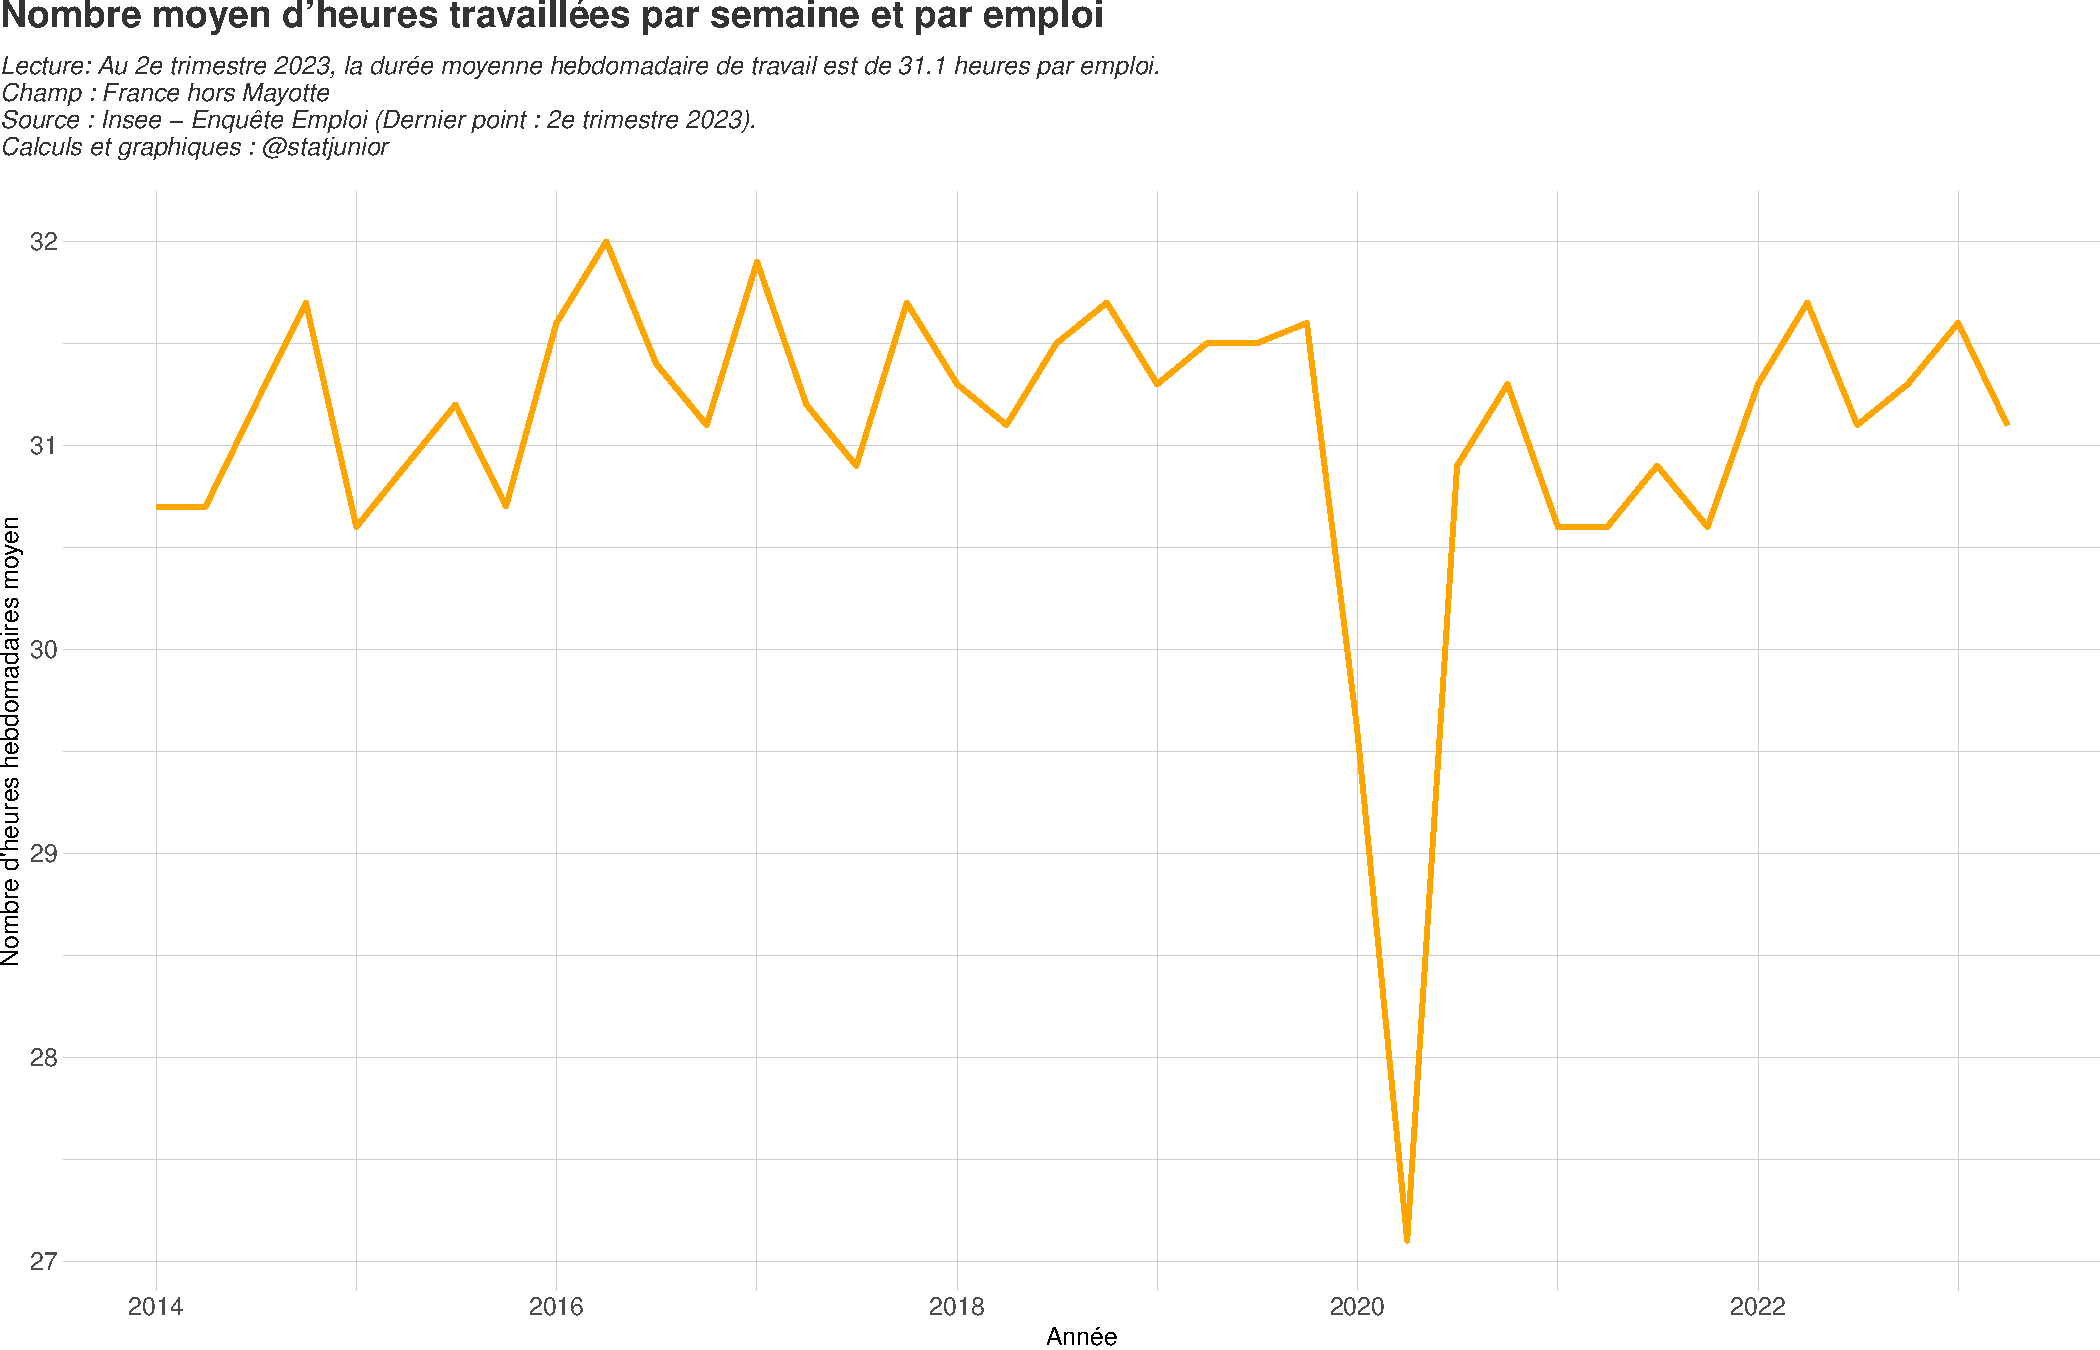
\includegraphics{rapport_activite_emploi_chomage_insee_files/figure-latex/unnamed-chunk-15-1.pdf}

\newpage

\hypertarget{taux-de-chuxf4mage-au-sens-du-bit}{%
\section{Taux de chômage au sens du
BIT}\label{taux-de-chuxf4mage-au-sens-du-bit}}

\hypertarget{chuxf4mage-au-sens-du-bit-et-taux-de-chuxf4mage-de-longue-duruxe9e}{%
\subsection{Chômage au sens du BIT et taux de chômage de longue
durée}\label{chuxf4mage-au-sens-du-bit-et-taux-de-chuxf4mage-de-longue-duruxe9e}}

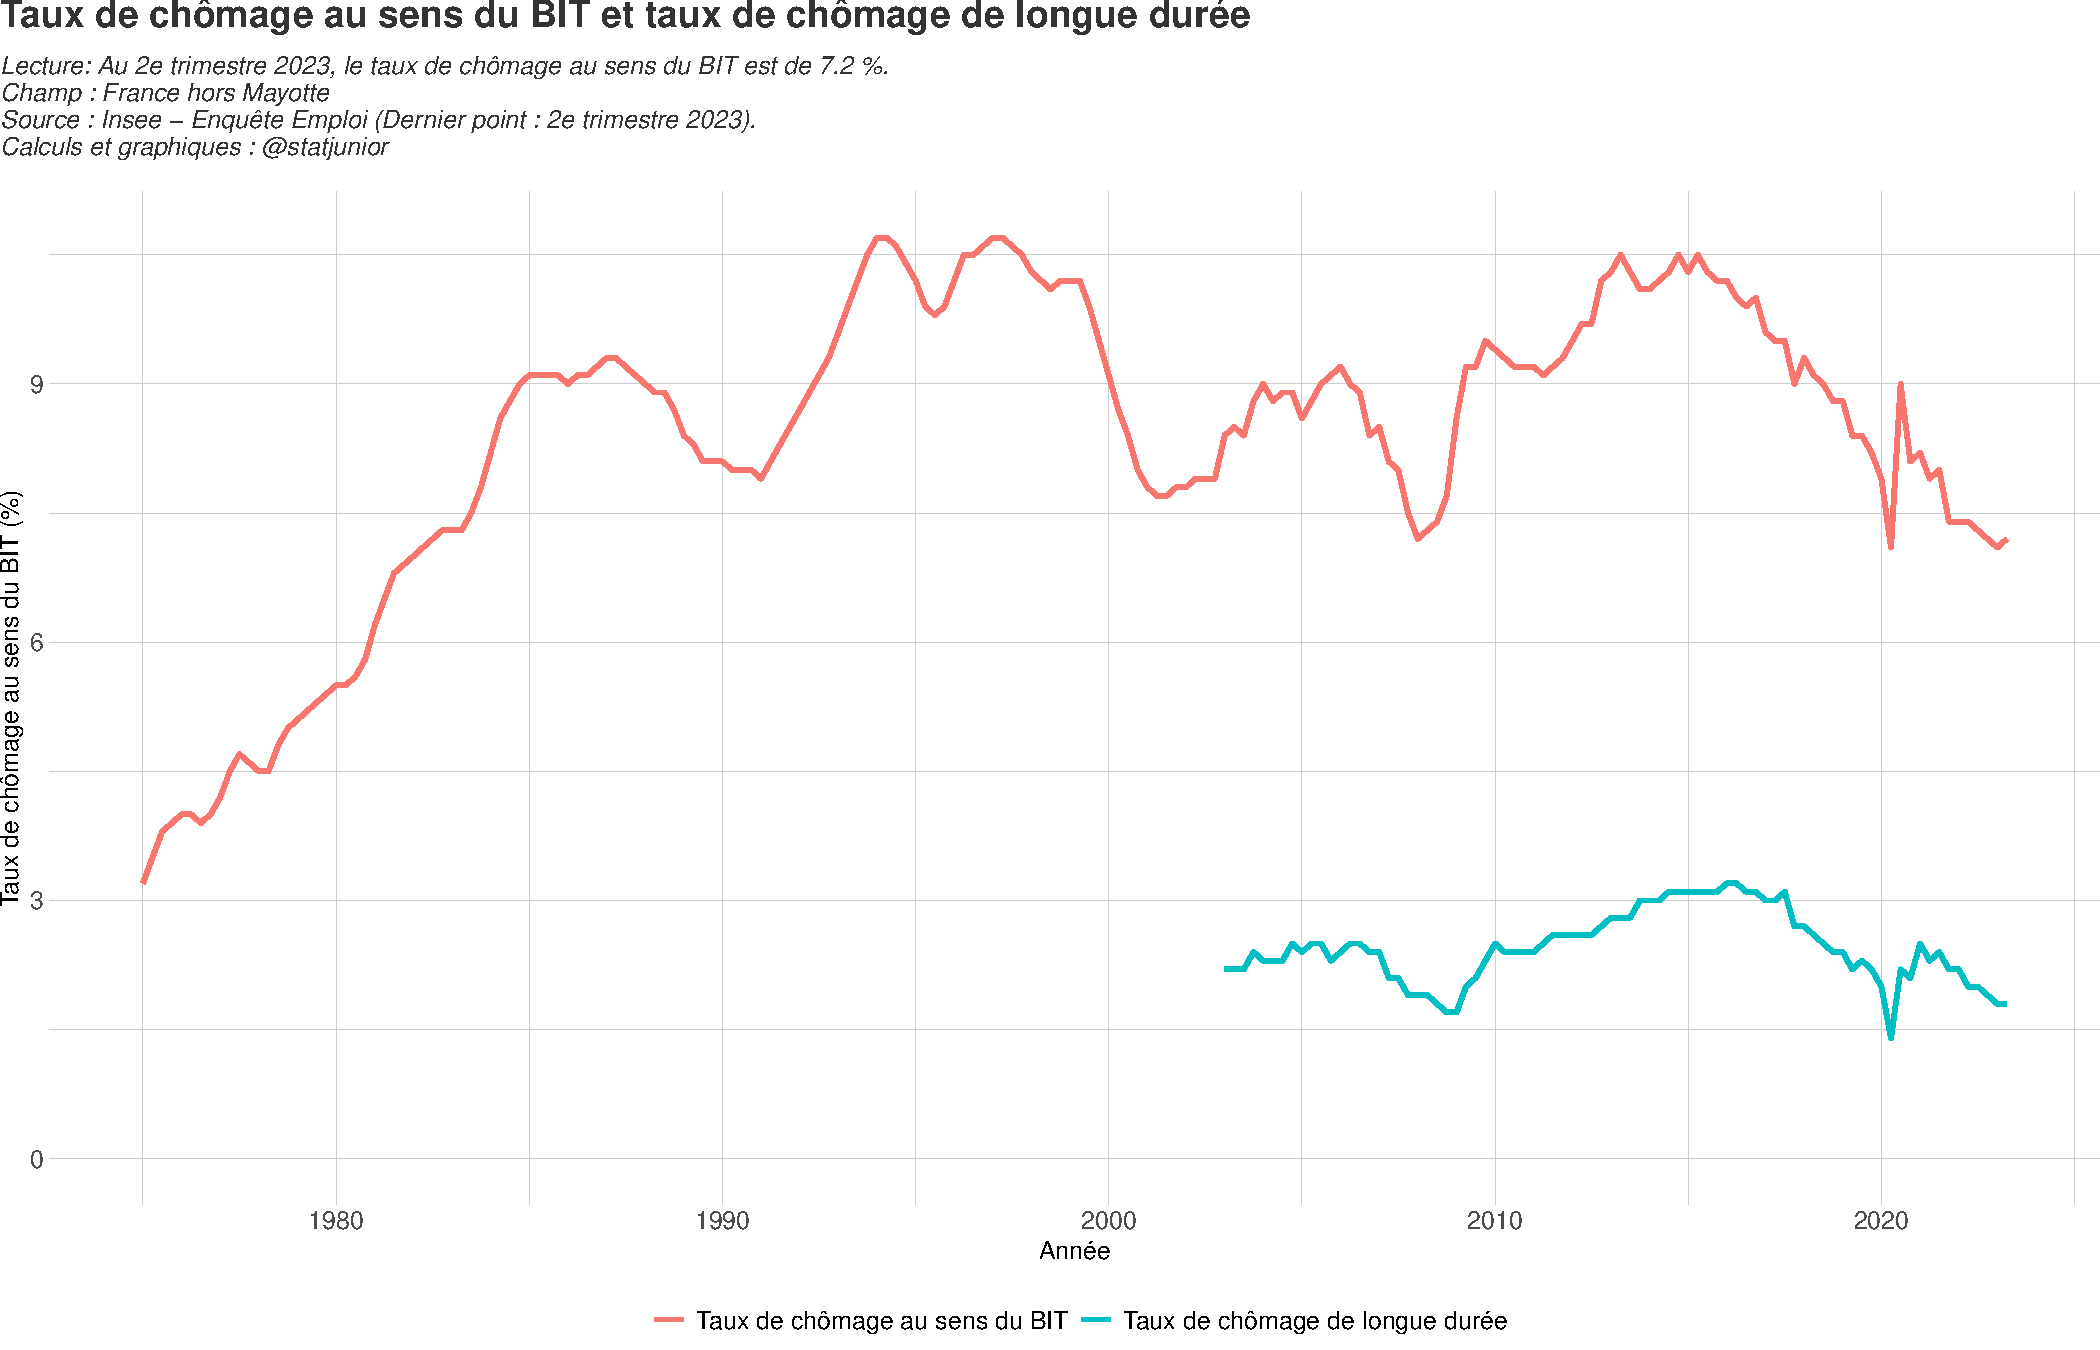
\includegraphics{rapport_activite_emploi_chomage_insee_files/figure-latex/unnamed-chunk-17-1.pdf}

\hypertarget{taux-de-chuxf4mage-bit-par-tranche-duxe2ge}{%
\subsection{Taux de chômage BIT par tranche
d'âge}\label{taux-de-chuxf4mage-bit-par-tranche-duxe2ge}}

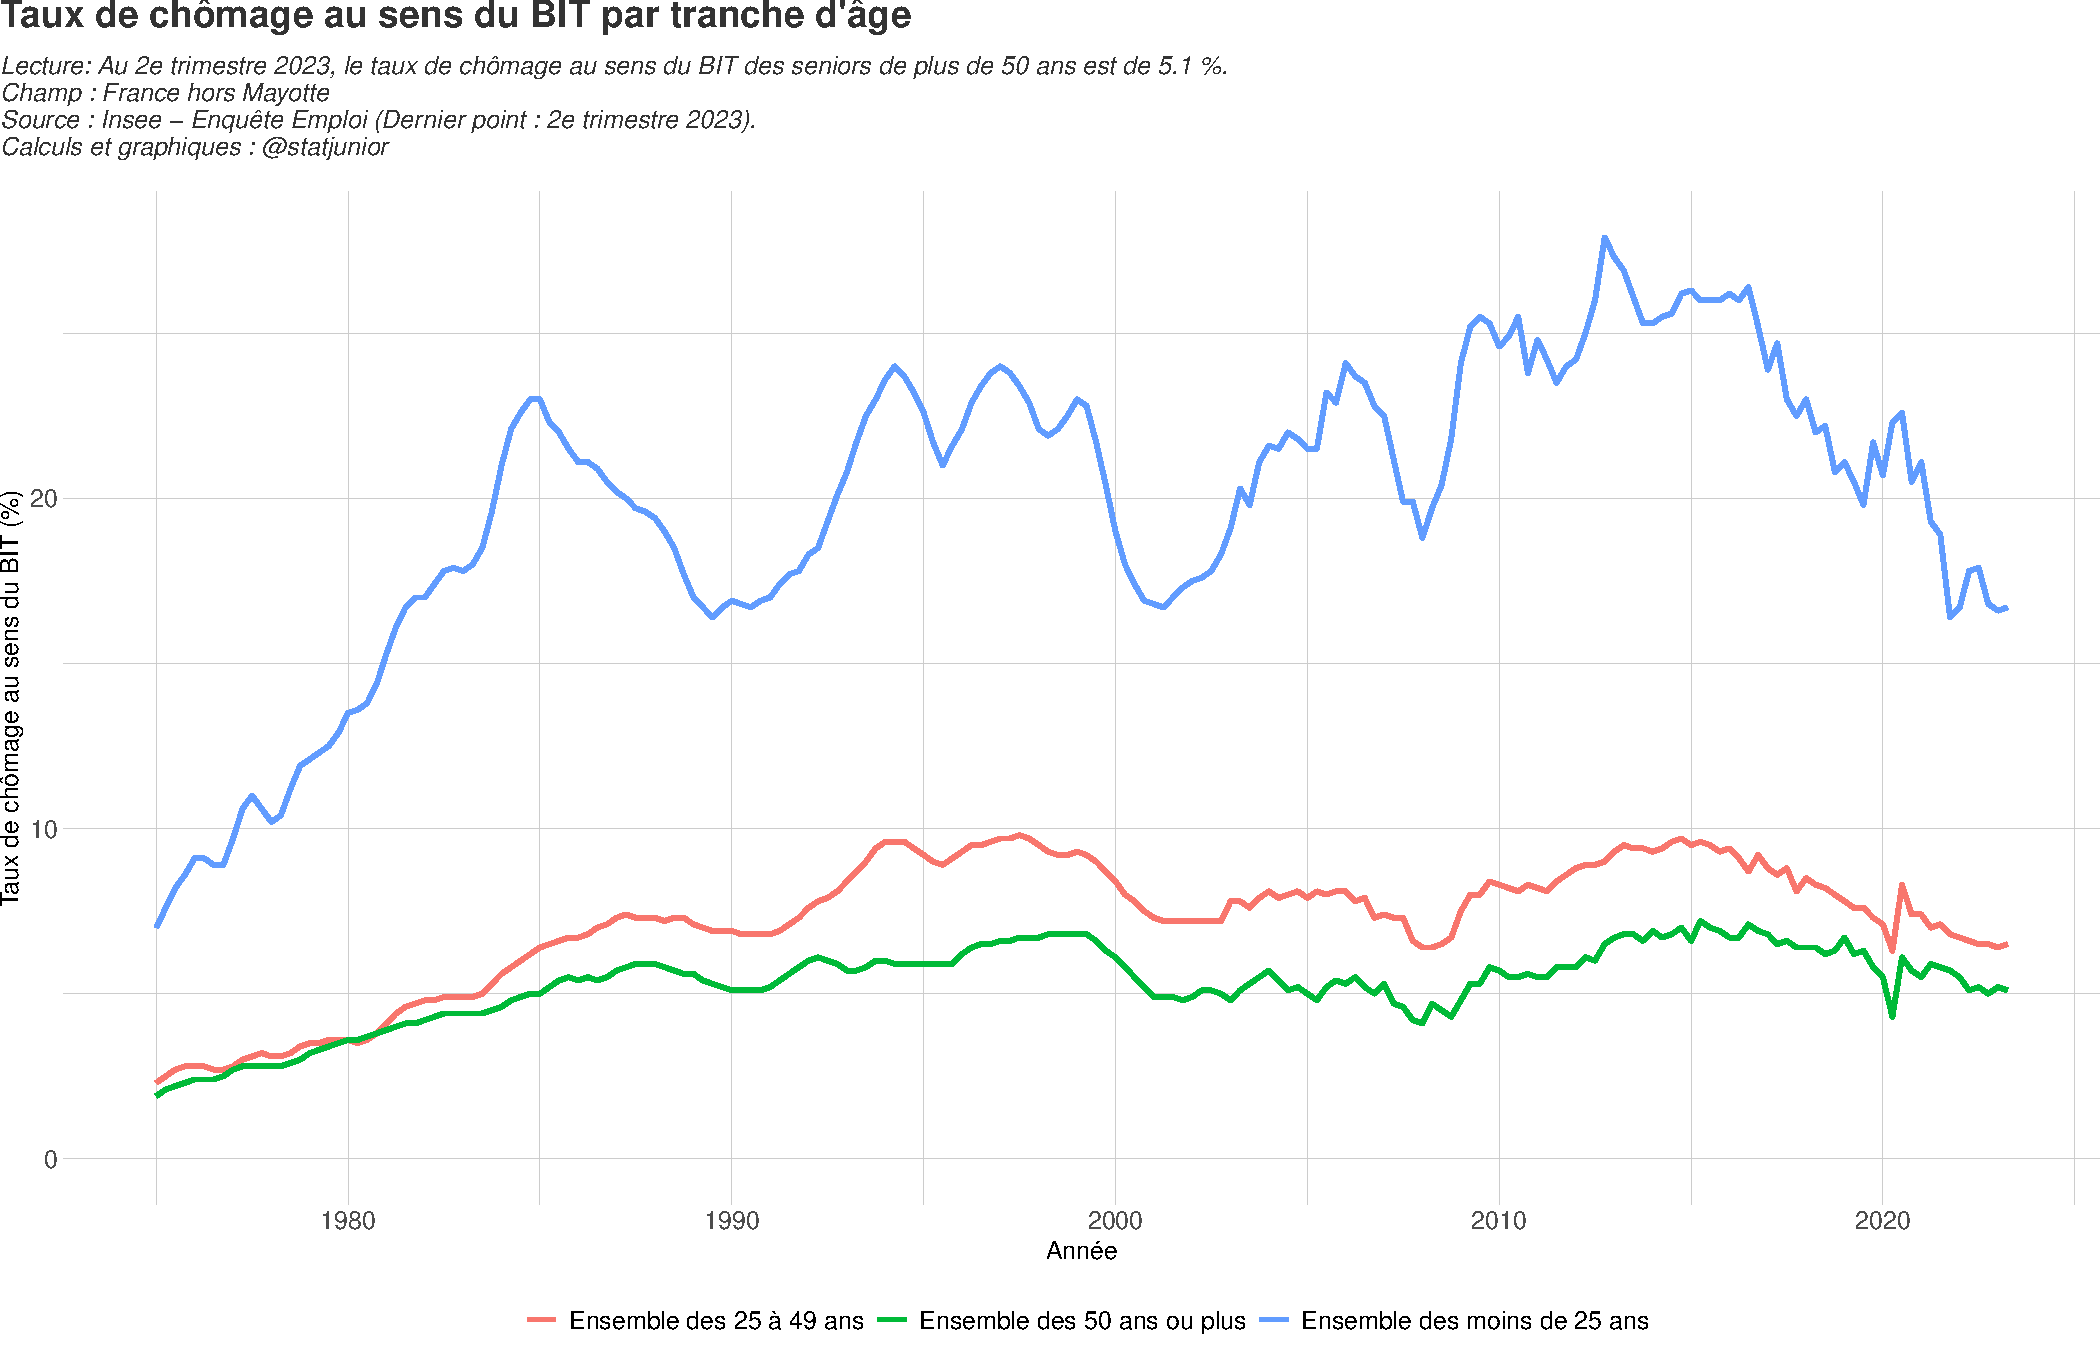
\includegraphics{rapport_activite_emploi_chomage_insee_files/figure-latex/unnamed-chunk-18-1.pdf}

\newpage

\hypertarget{taux-de-chuxf4mage-uxe9largi-bit-halo-du-chuxf4mage-sous-emploi-involontaire}{%
\section{Taux de chômage élargi (BIT + halo du chômage + sous-emploi
involontaire)}\label{taux-de-chuxf4mage-uxe9largi-bit-halo-du-chuxf4mage-sous-emploi-involontaire}}

\hypertarget{en-proportion-des-participants-au-marchuxe9-du-travail}{%
\subsection{En proportion des participants au marché du
travail}\label{en-proportion-des-participants-au-marchuxe9-du-travail}}

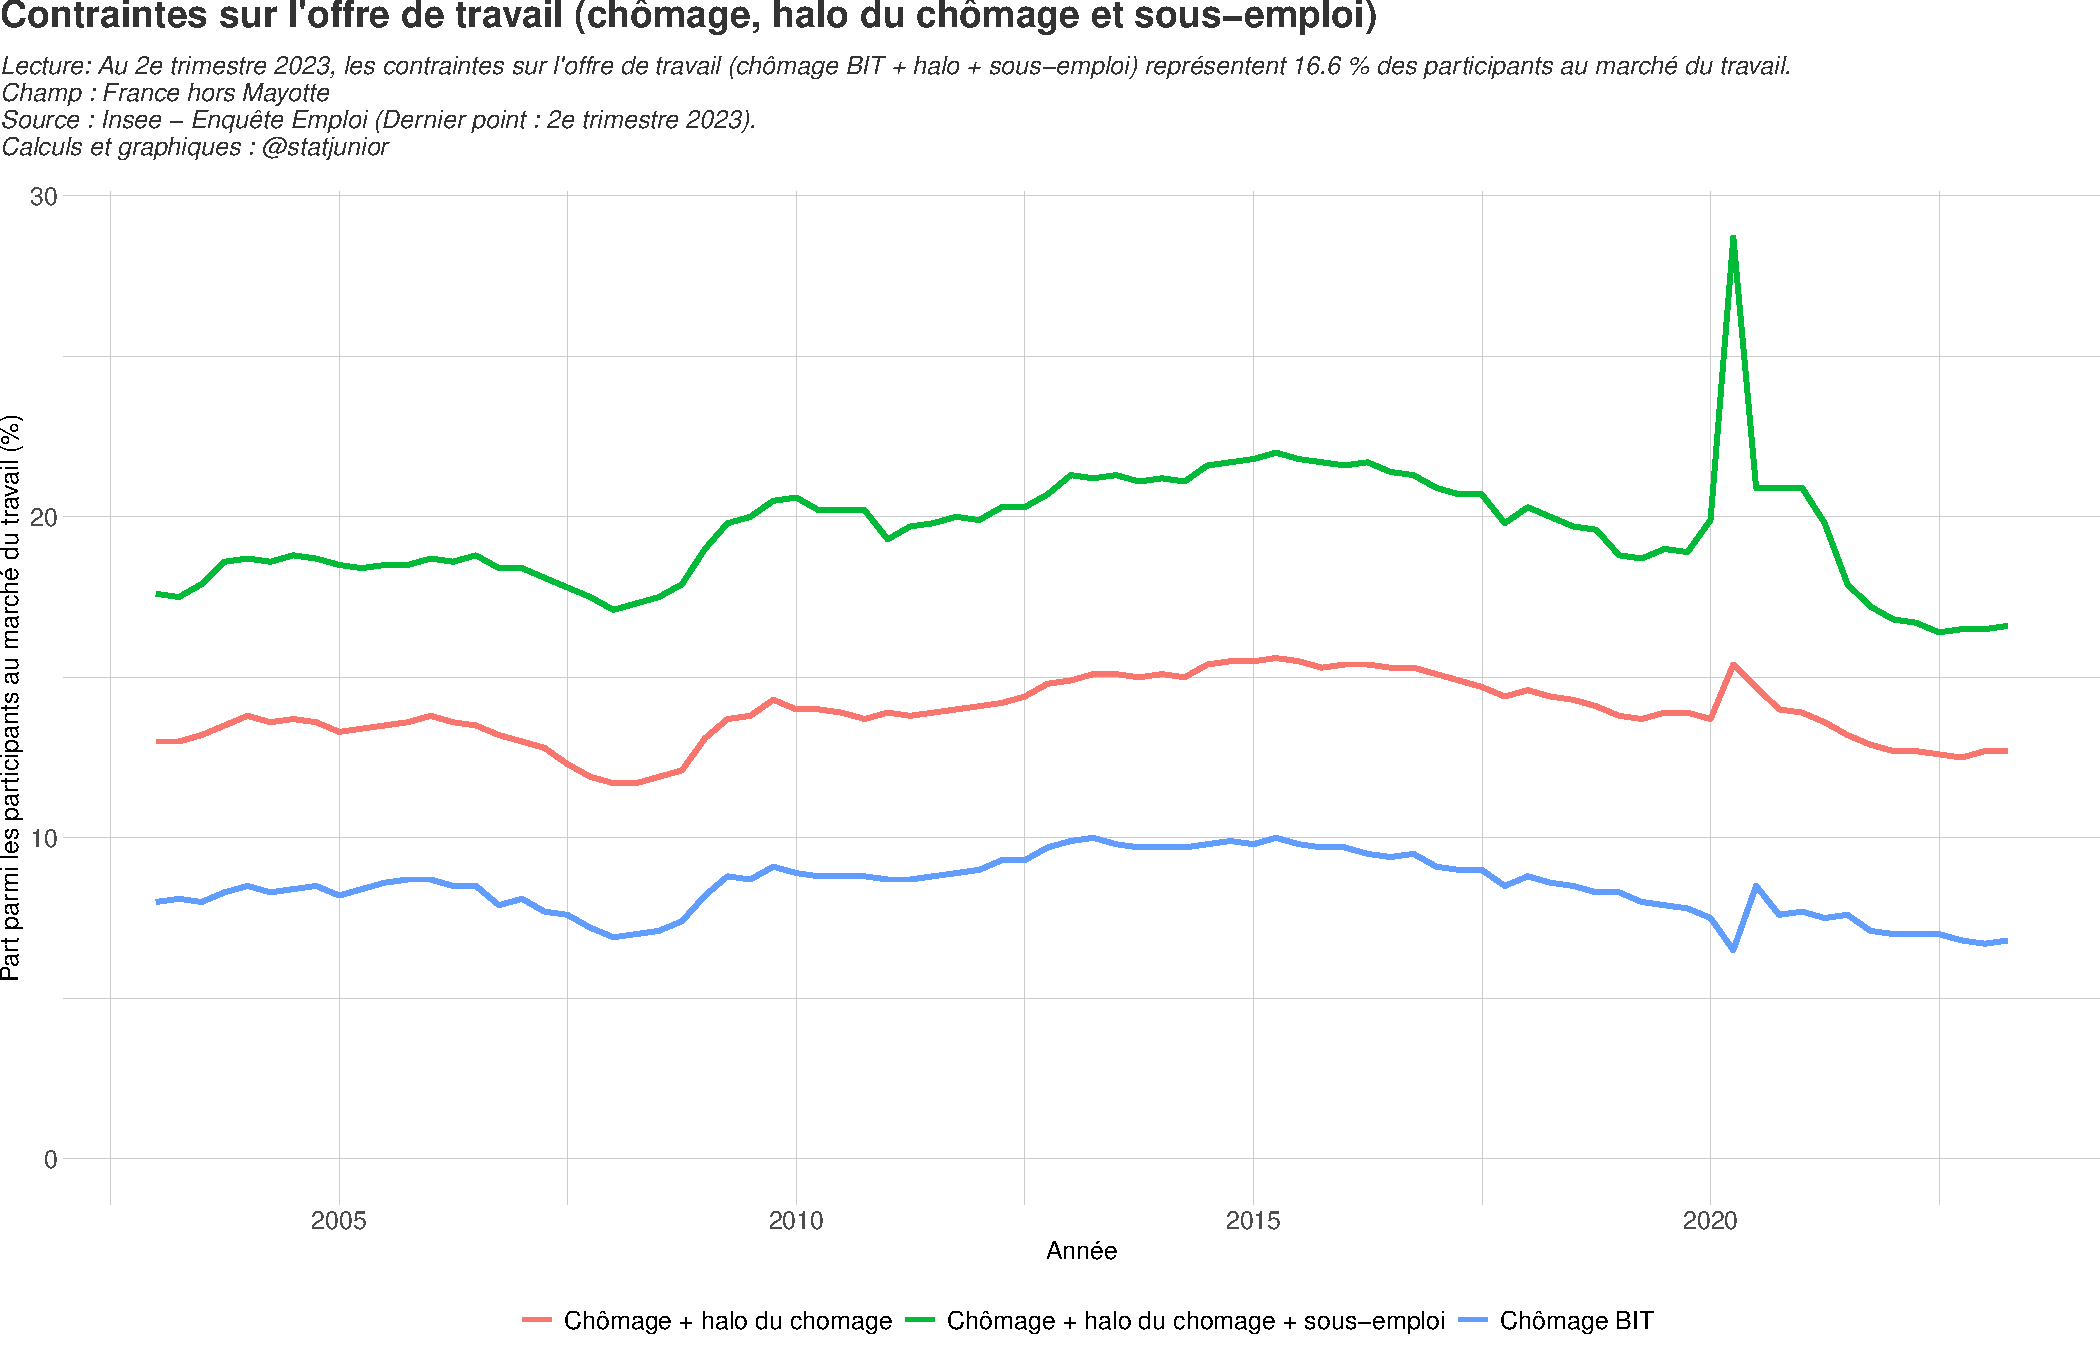
\includegraphics{rapport_activite_emploi_chomage_insee_files/figure-latex/unnamed-chunk-20-1.pdf}

\hypertarget{halo-du-chuxf4mage-par-tranche-dage}{%
\subsection{Halo du chômage par tranche
d'age}\label{halo-du-chuxf4mage-par-tranche-dage}}

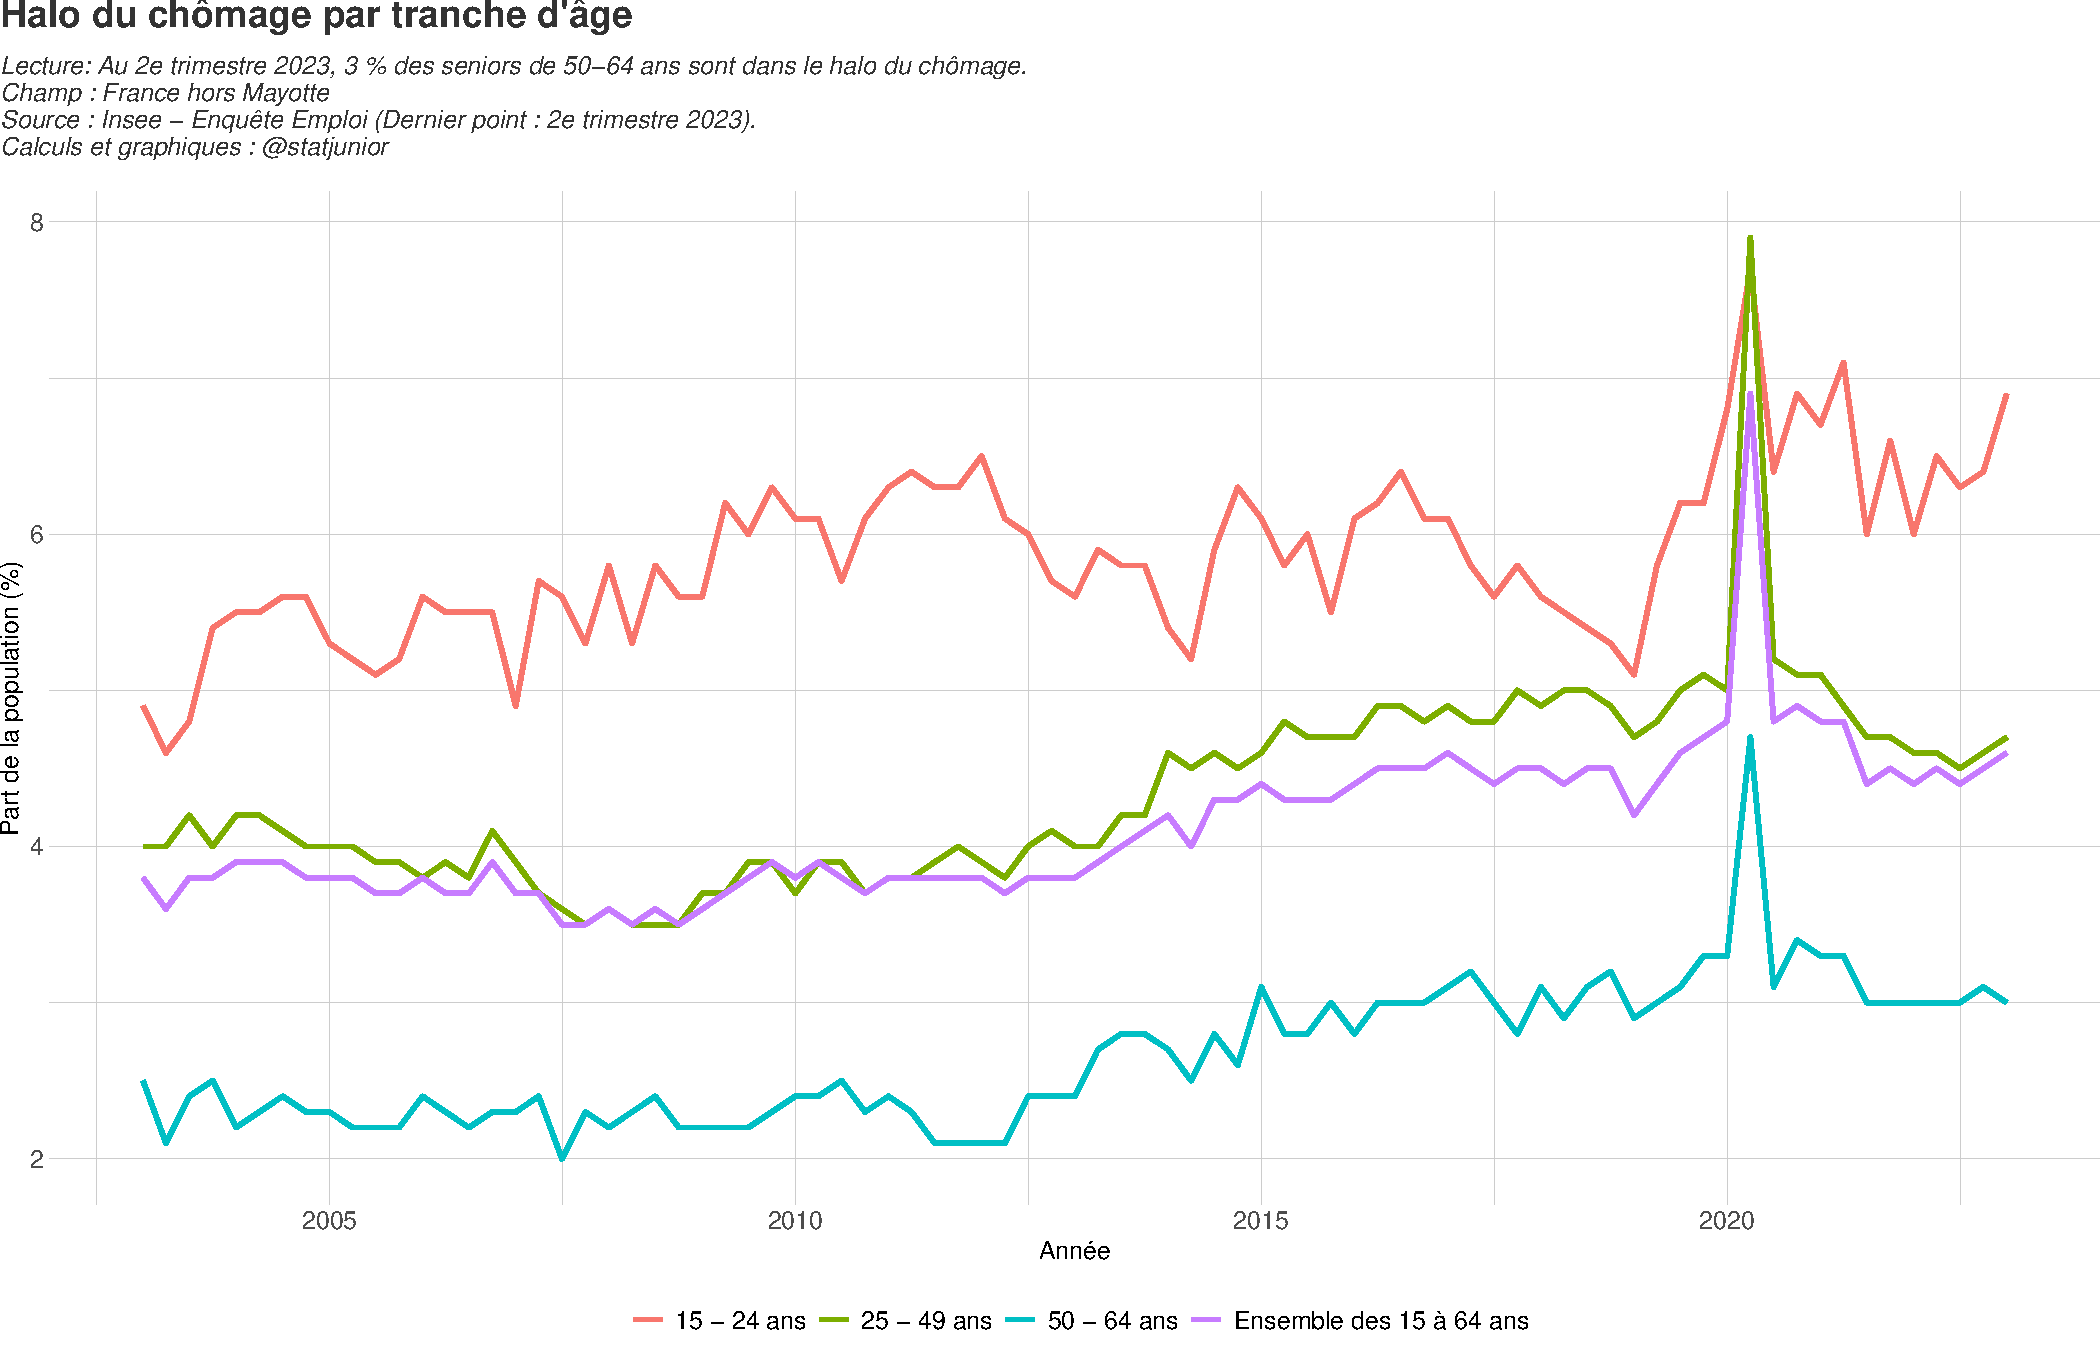
\includegraphics{rapport_activite_emploi_chomage_insee_files/figure-latex/unnamed-chunk-21-1.pdf}

\newpage

\hypertarget{nombre-de-personnes-au-chuxf4mage-ou-ayant-des-contraintes-demploi-halo-sous-emploi}{%
\section{Nombre de personnes au chômage ou ayant des contraintes
d'emploi (halo,
sous-emploi)}\label{nombre-de-personnes-au-chuxf4mage-ou-ayant-des-contraintes-demploi-halo-sous-emploi}}

\hypertarget{nombre-de-personnes-au-chomage-bit-ou-dans-le-halo}{%
\subsection{Nombre de personnes au chomage BIT ou dans le
halo}\label{nombre-de-personnes-au-chomage-bit-ou-dans-le-halo}}

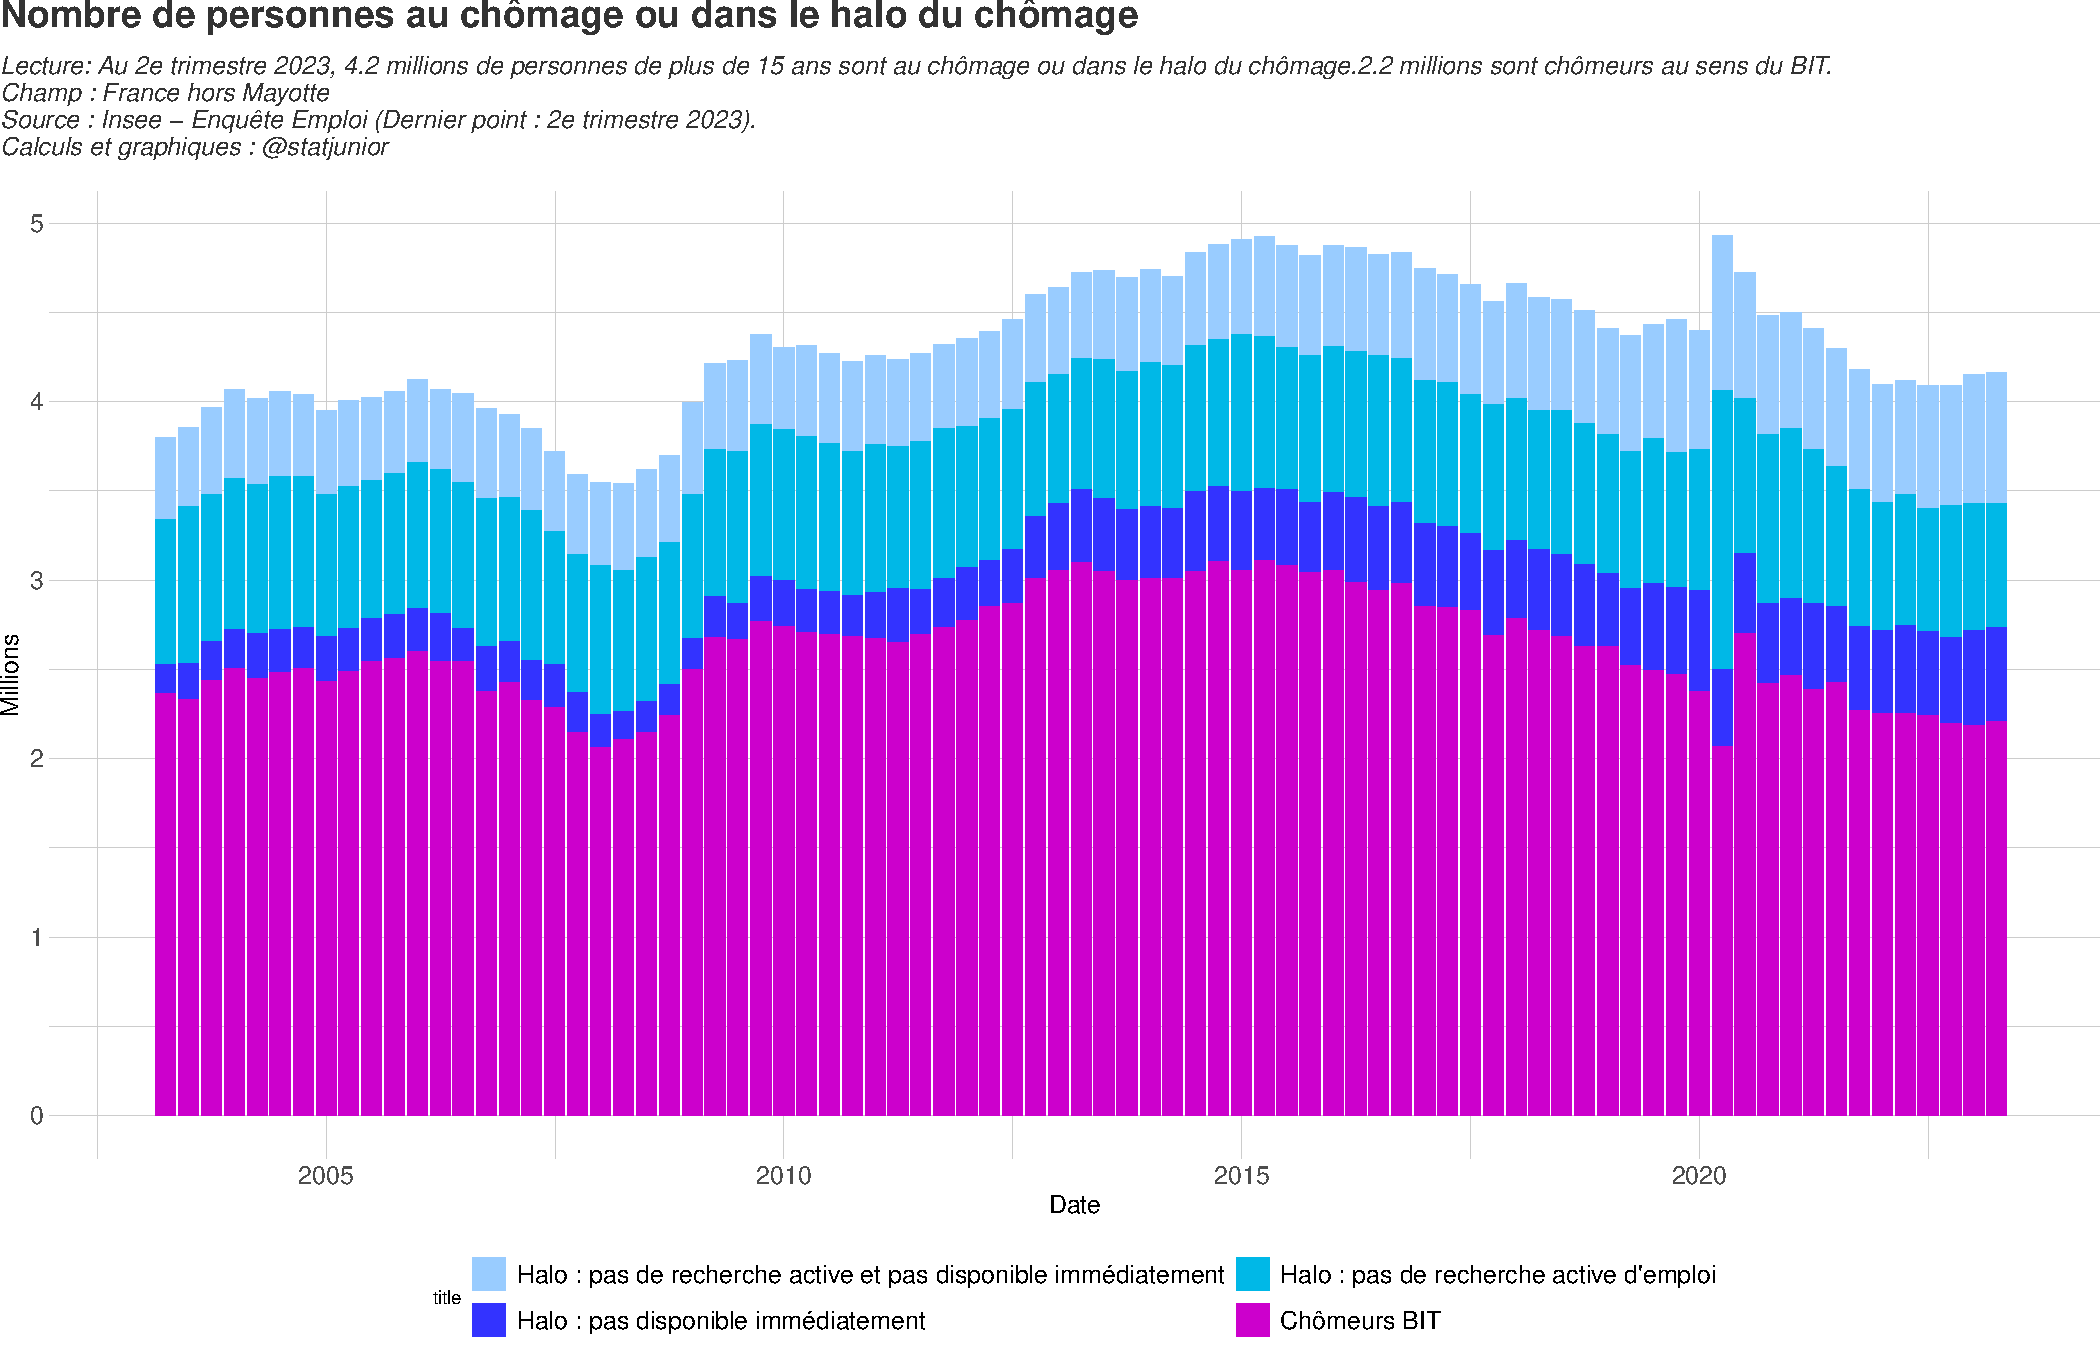
\includegraphics{rapport_activite_emploi_chomage_insee_files/figure-latex/unnamed-chunk-23-1.pdf}

\hypertarget{part-des-personnes-comptuxe9es-comme-chuxf4meurs-bit-parmi-les-chuxf4meurs-semi-uxe9largis-bit-halo-du-chomage}{%
\subsection{Part des personnes comptées comme chômeurs BIT parmi les
chômeurs semi-élargis (BIT + halo du
chomage)}\label{part-des-personnes-comptuxe9es-comme-chuxf4meurs-bit-parmi-les-chuxf4meurs-semi-uxe9largis-bit-halo-du-chomage}}

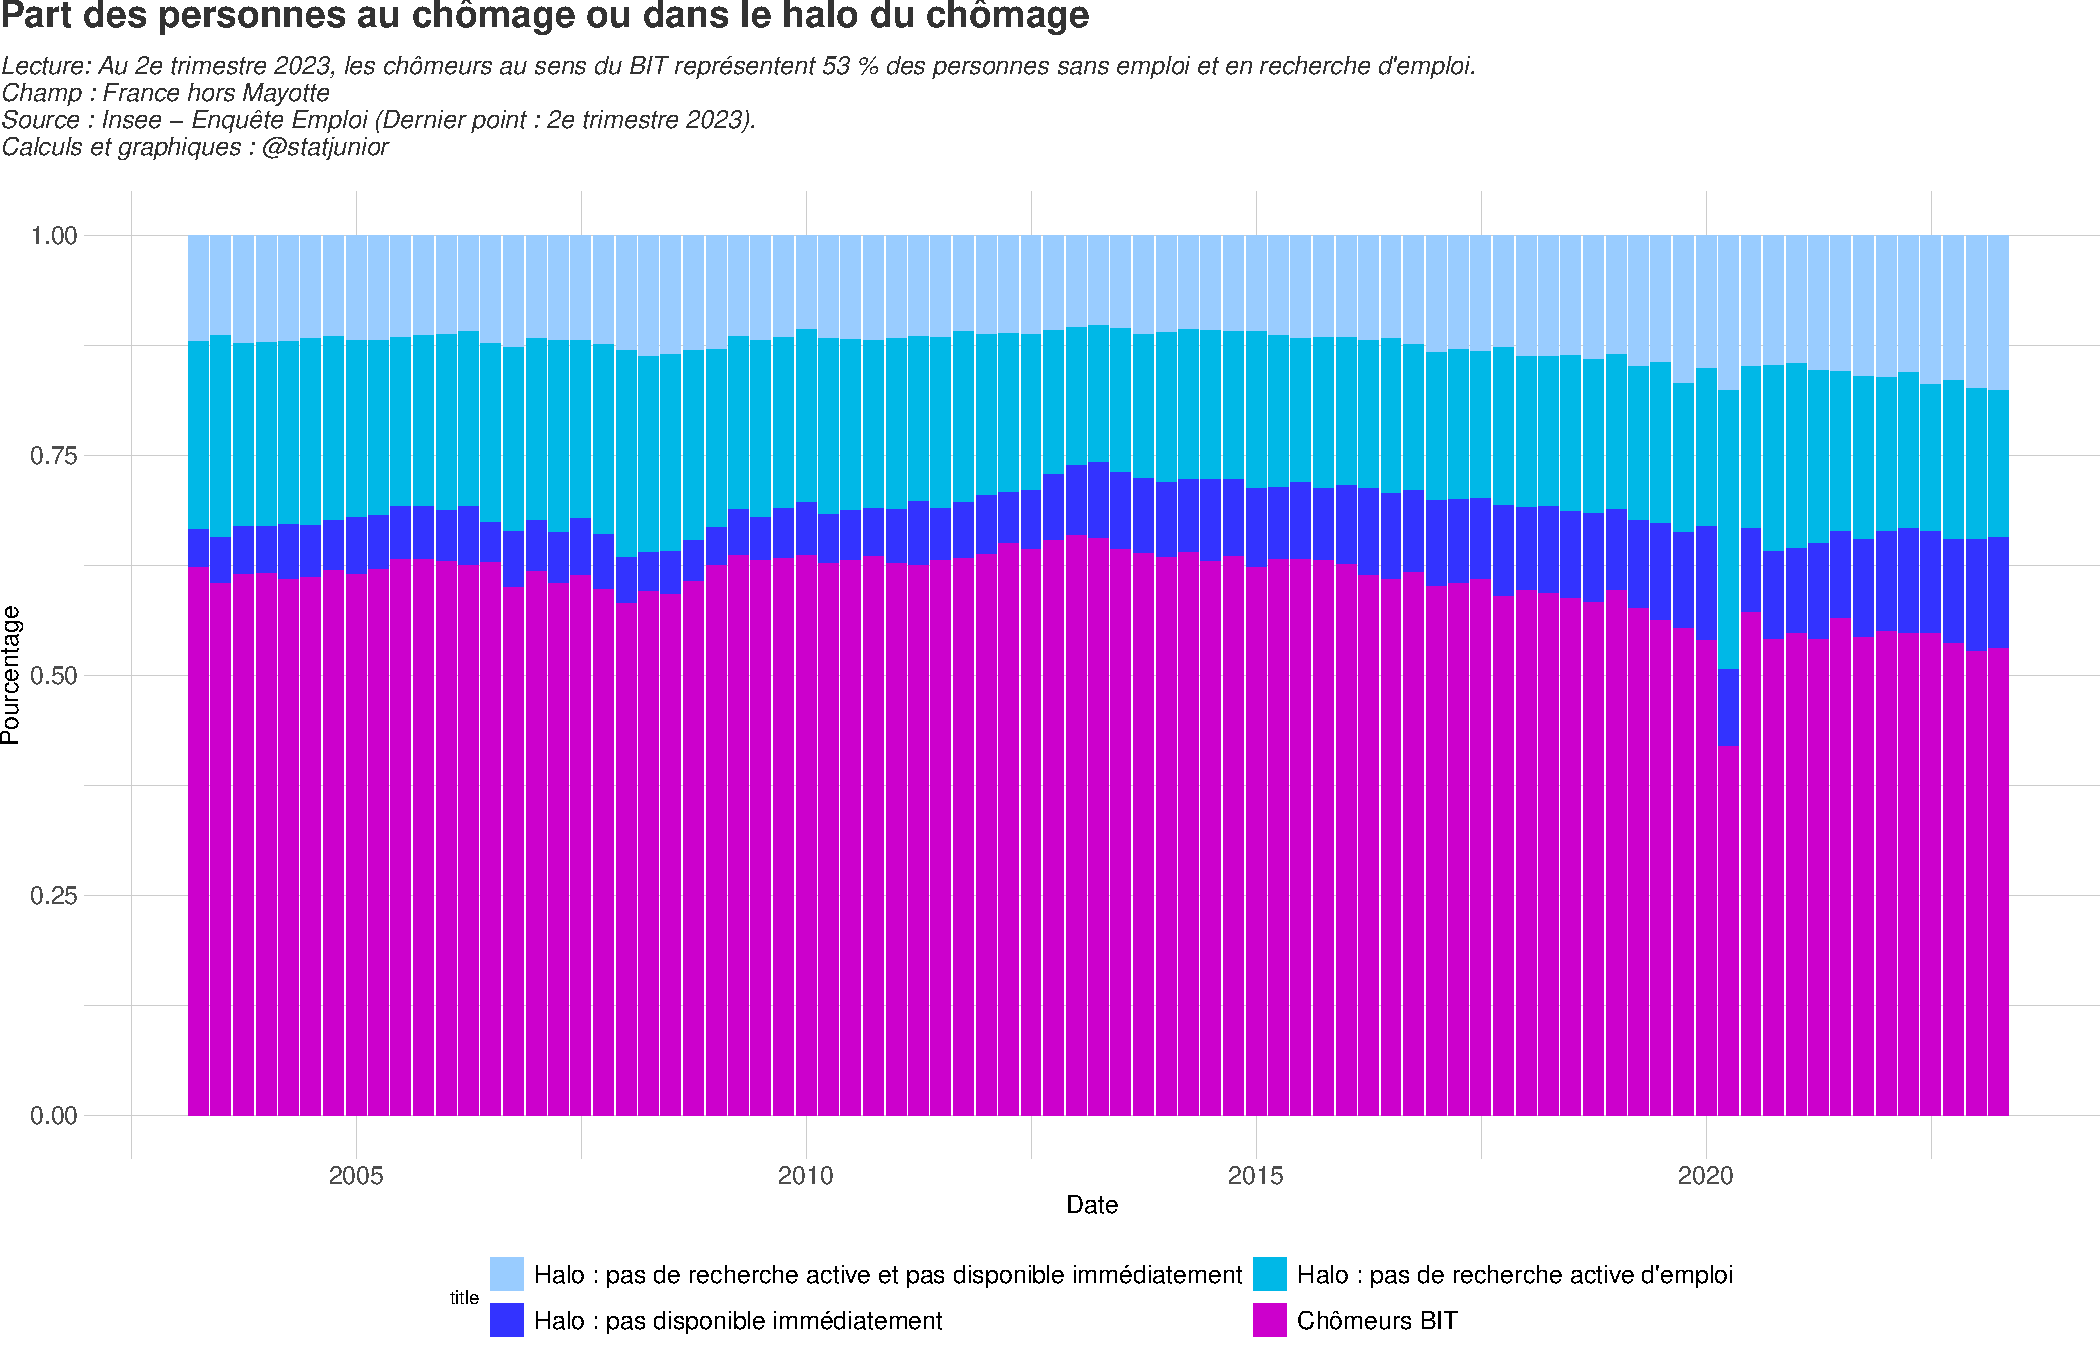
\includegraphics{rapport_activite_emploi_chomage_insee_files/figure-latex/unnamed-chunk-24-1.pdf}

\hypertarget{nombre-de-personnes-dans-le-halo-du-chuxf4mage}{%
\subsection{Nombre de personnes dans le halo du
chômage}\label{nombre-de-personnes-dans-le-halo-du-chuxf4mage}}

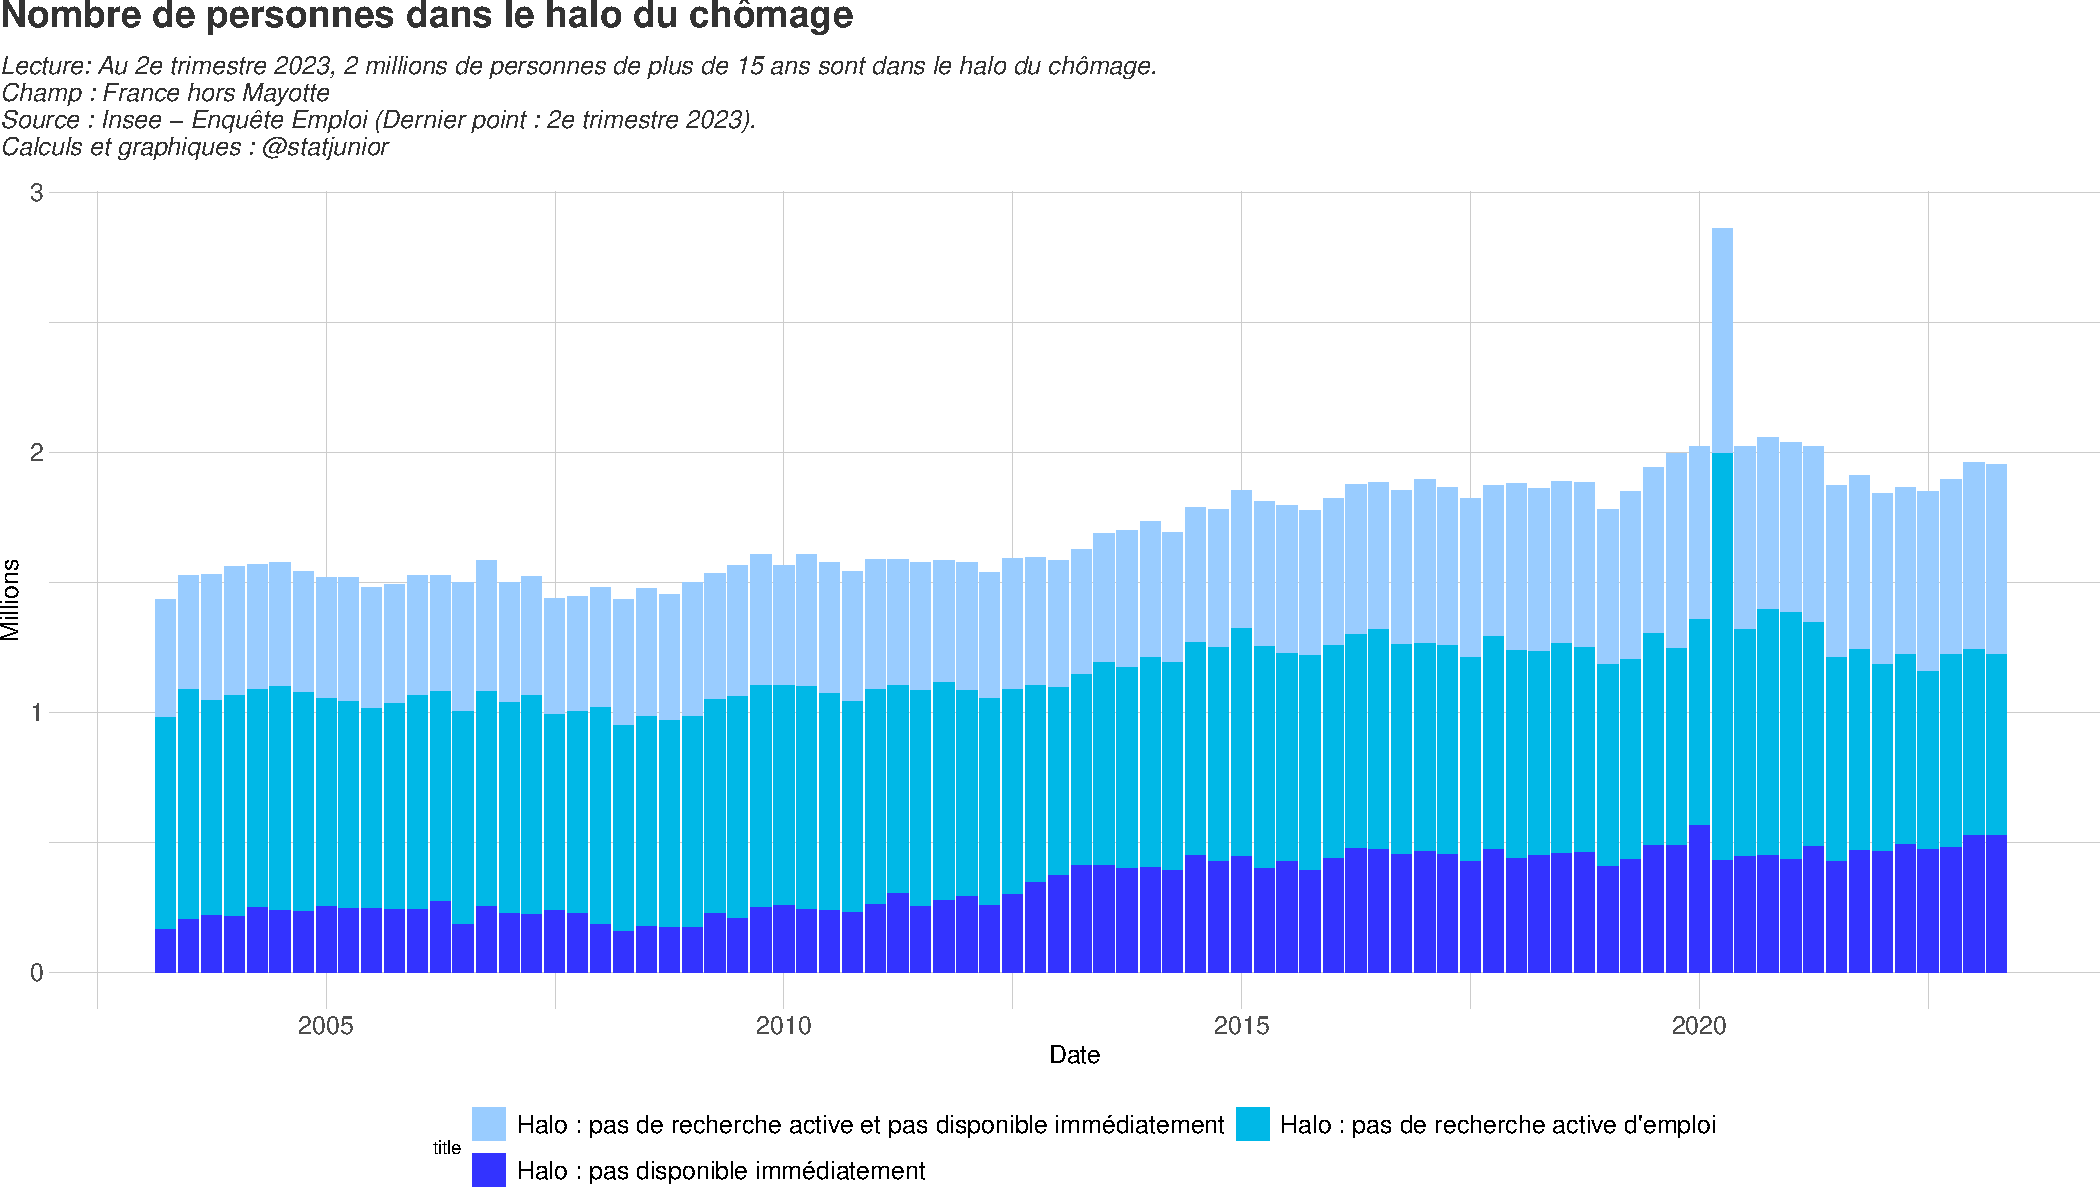
\includegraphics{rapport_activite_emploi_chomage_insee_files/figure-latex/unnamed-chunk-25-1.pdf}

\hypertarget{nombre-de-personnes-en-sous-emploi}{%
\subsection{Nombre de personnes en
sous-emploi}\label{nombre-de-personnes-en-sous-emploi}}

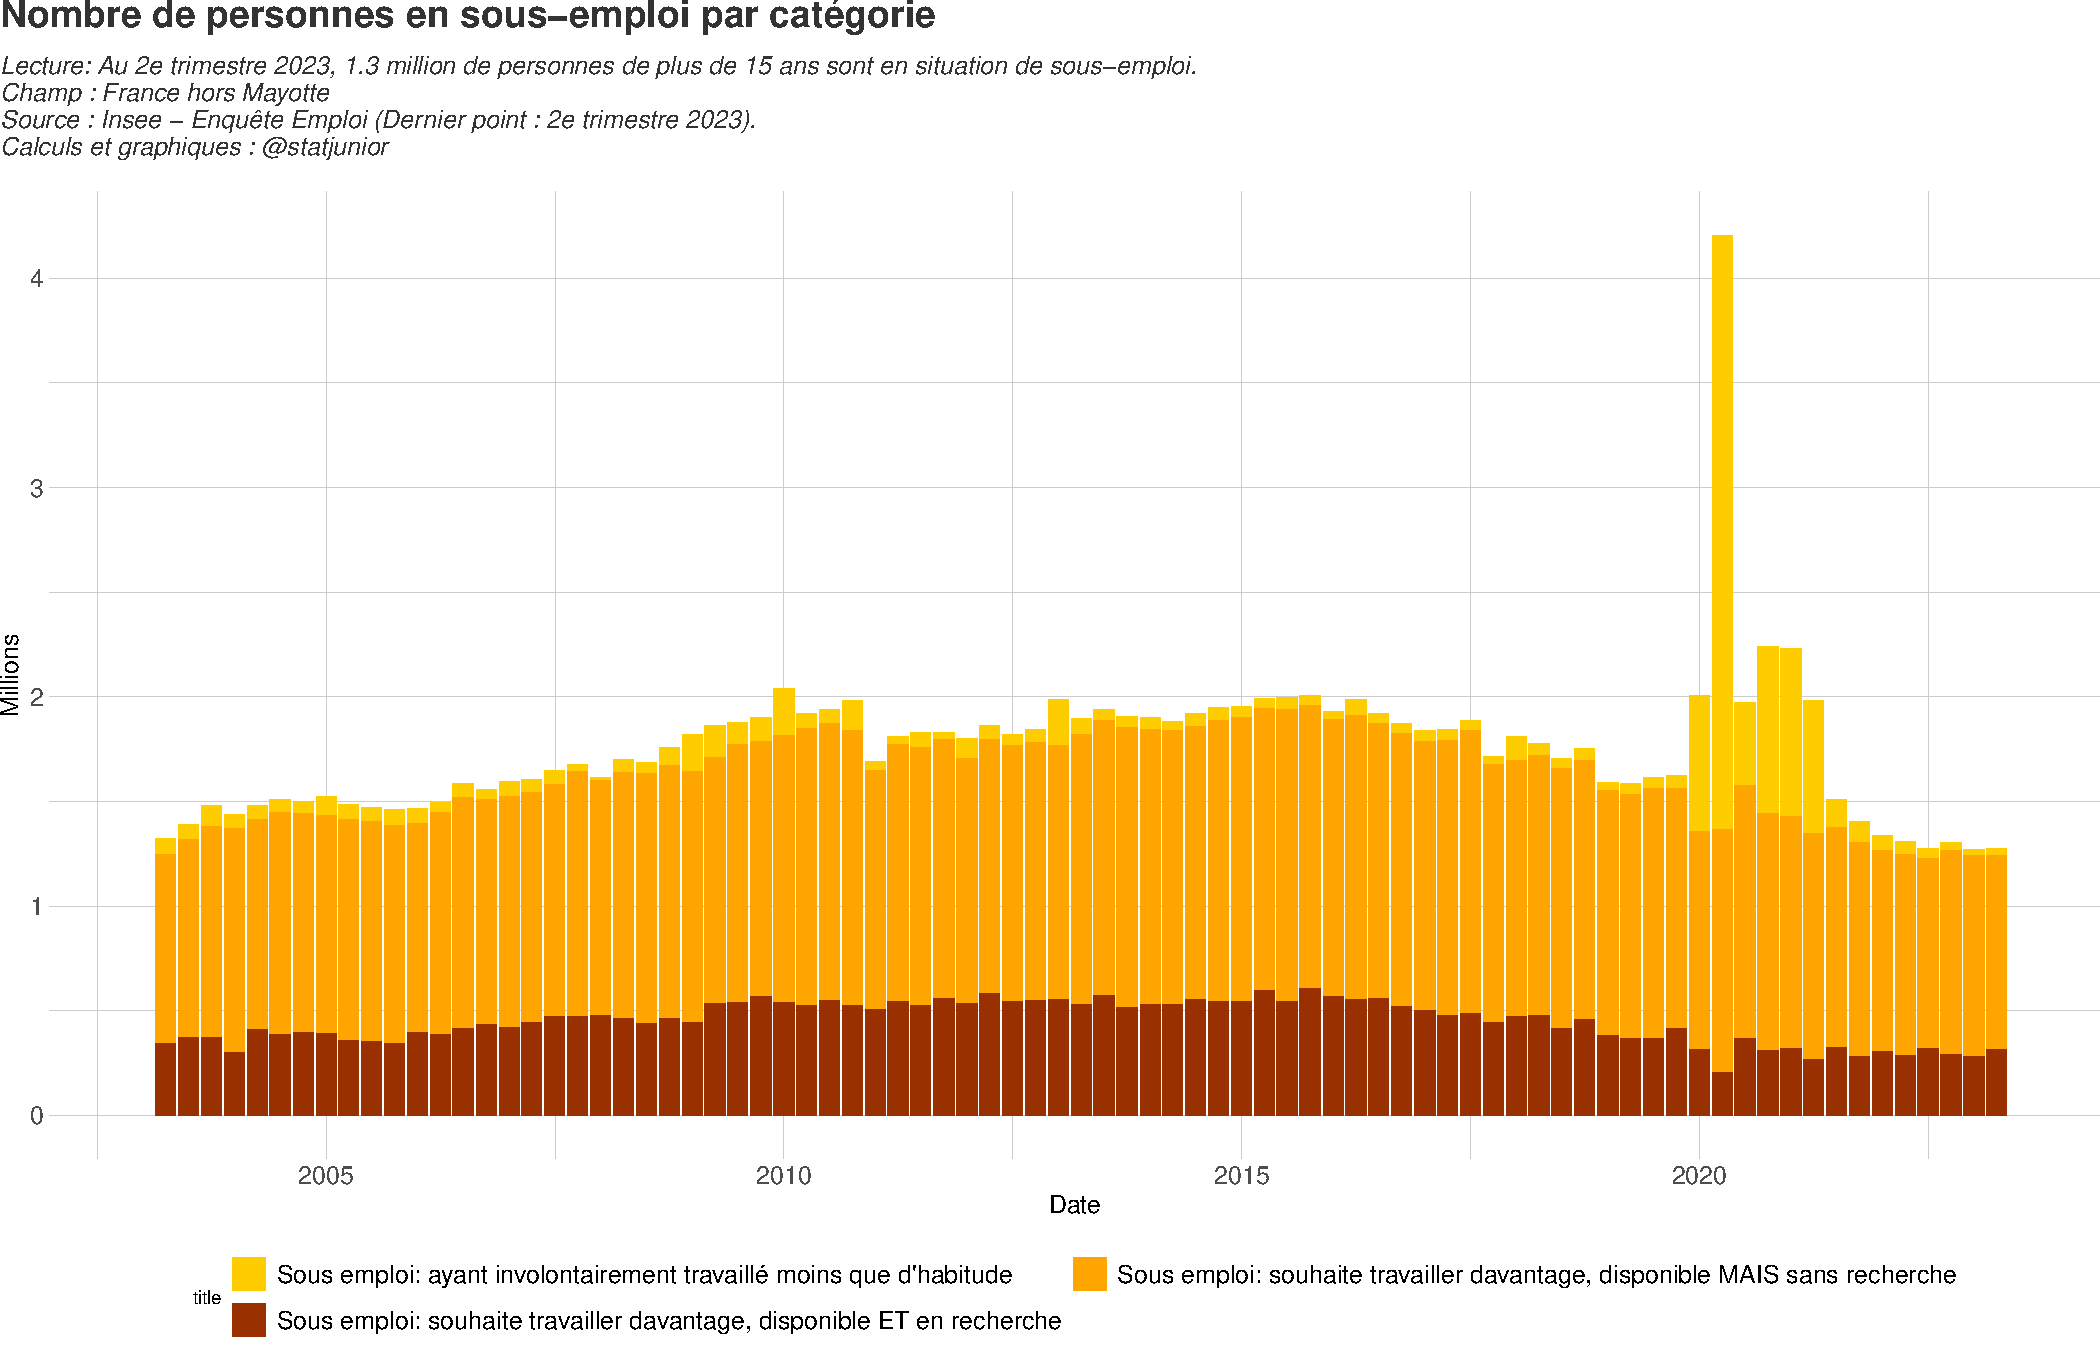
\includegraphics{rapport_activite_emploi_chomage_insee_files/figure-latex/unnamed-chunk-28-1.pdf}

\hypertarget{nombre-total-de-personnes-exprimant-des-contraintes-demploi-chuxf4meurs-bit-halo-du-chomage-et-sous-emploi}{%
\subsection{Nombre total de personnes exprimant des contraintes d'emploi
: chômeurs BIT, halo du chomage et
sous-emploi}\label{nombre-total-de-personnes-exprimant-des-contraintes-demploi-chuxf4meurs-bit-halo-du-chomage-et-sous-emploi}}

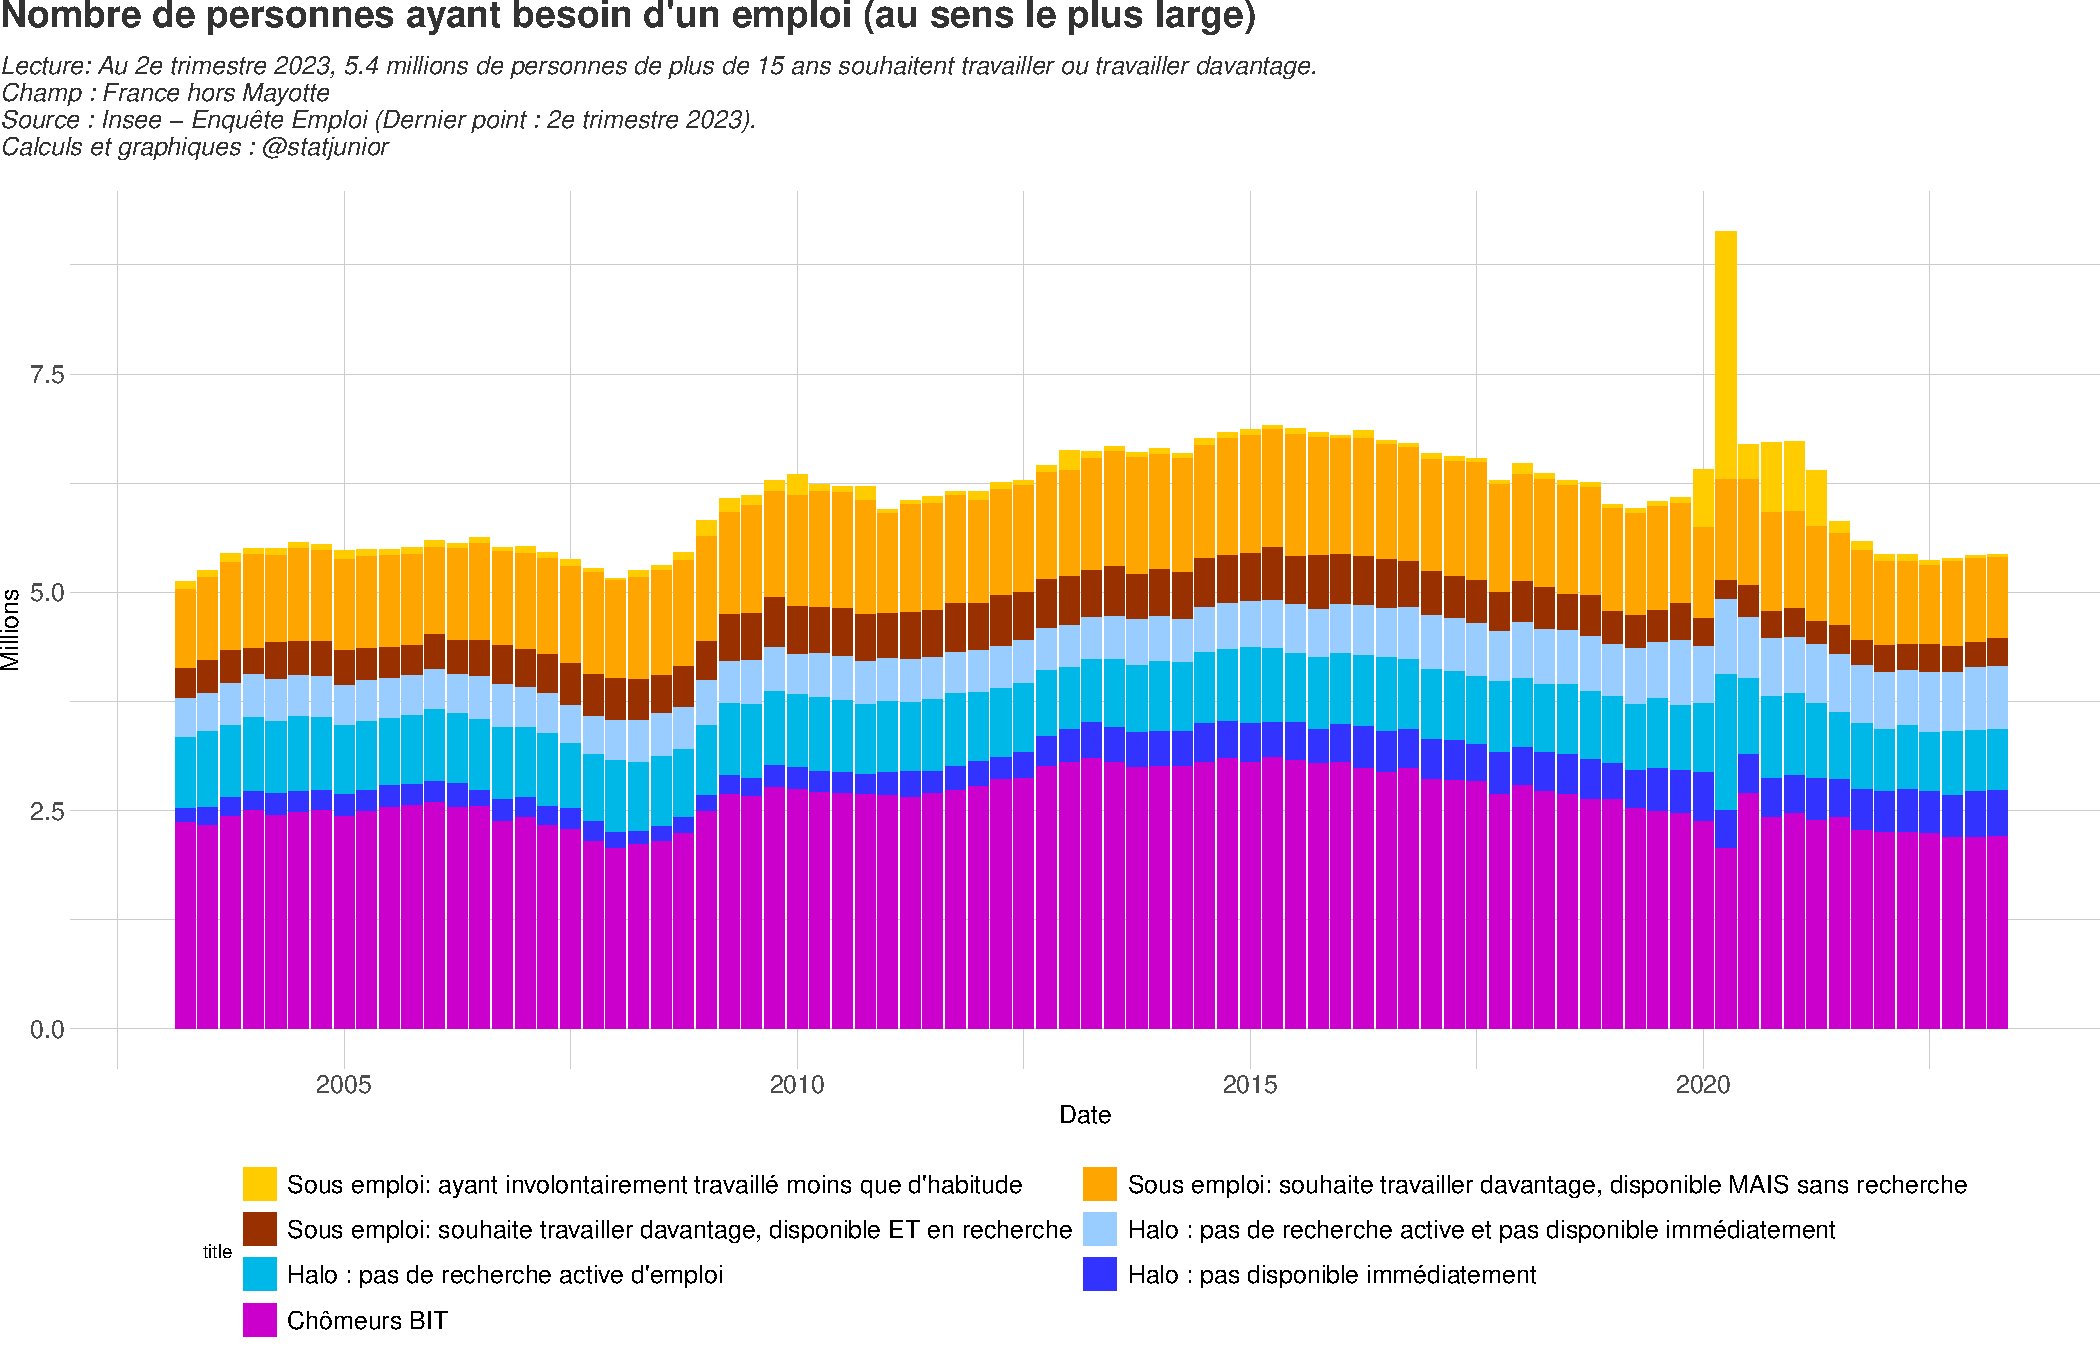
\includegraphics{rapport_activite_emploi_chomage_insee_files/figure-latex/unnamed-chunk-29-1.pdf}

\hypertarget{la-confrontation-des-sources-administratives-dares-puxf4le-emploi-avec-lenquuxeate-emploi-chuxf4mage-bit-insee}{%
\section{La confrontation des sources administratives (Dares-Pôle
Emploi) avec l'enquête Emploi (chômage
BIT-Insee)}\label{la-confrontation-des-sources-administratives-dares-puxf4le-emploi-avec-lenquuxeate-emploi-chuxf4mage-bit-insee}}

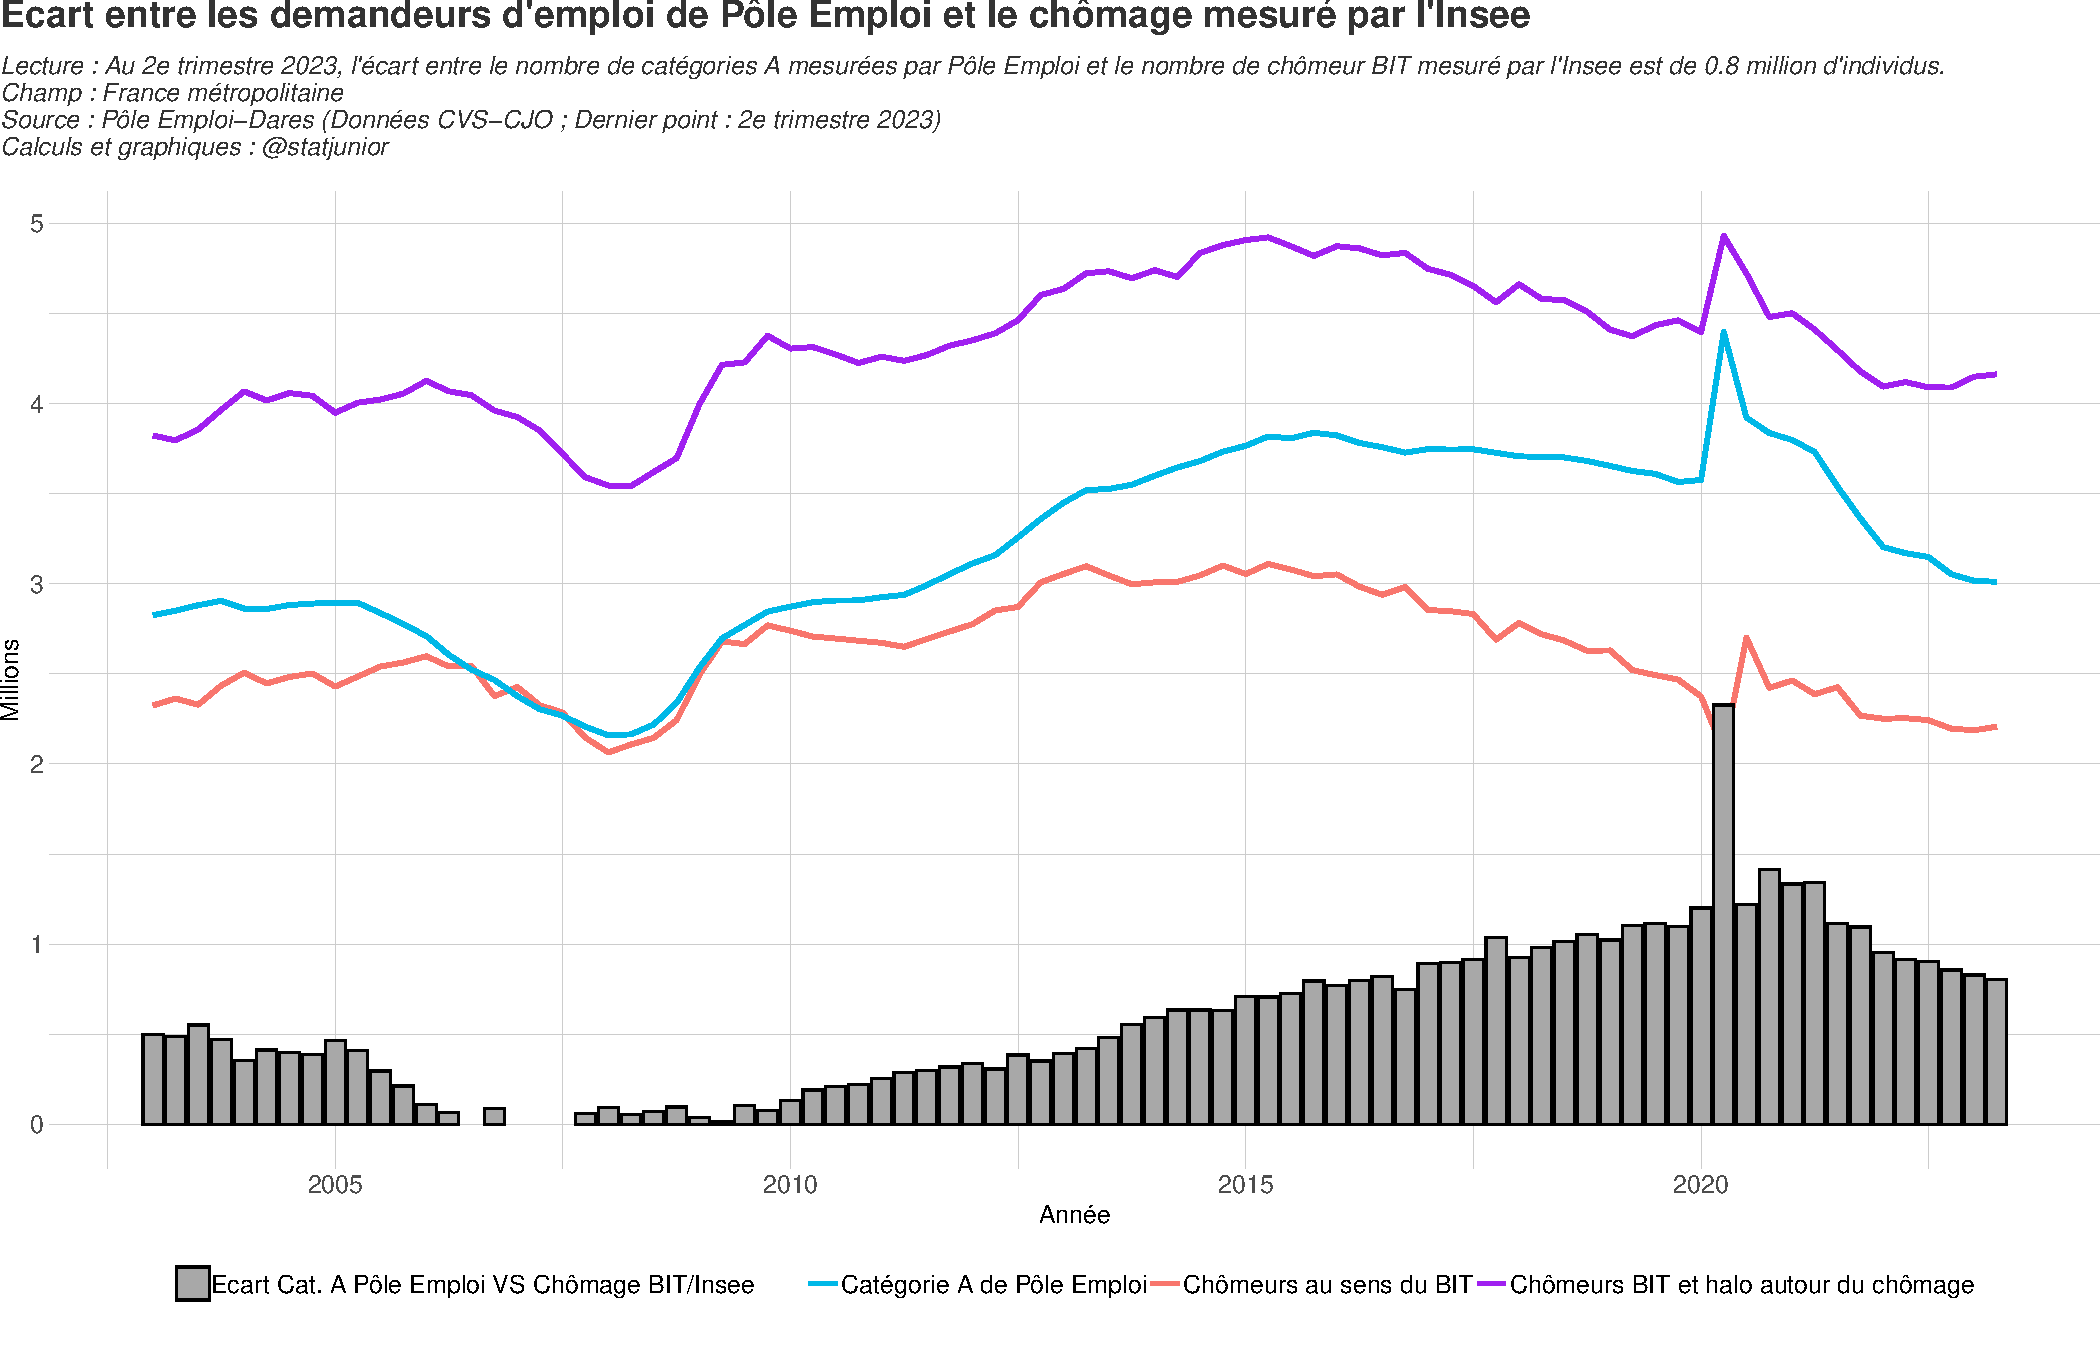
\includegraphics{rapport_activite_emploi_chomage_insee_files/figure-latex/unnamed-chunk-31-1.pdf}

\end{document}
